\documentclass[12pt]{book}
\usepackage[margin=1 in]{geometry}
\usepackage[english]{babel}
\usepackage[T1]{fontenc}
\usepackage{times}
\usepackage{graphicx,tikz,amsmath,caption,enumitem,subfig,hyperref,xfrac,color,tikzscale,circuitikz}
\usepackage[version-1-compatibility]{siunitx}
\usepackage[version=3]{mhchem}
\usepackage[makeroom]{cancel}
\usepackage{subfiles}
\setcounter{tocdepth}{3}
\usepackage{siunitx}
\PassOptionsToPackage{version=3}{mhchem}


%\graphicspath{ {G:/Dropbox/work/Phd/Data/Xujie Chen_data_on_Li-air/EIS paper/Raw Plots/735457/} }

\begin{document}
\title{Mohit Mehta's Research Notebook}
\author{Mohit Mehta}
\date{\today}
\maketitle
\tableofcontents
\chapter{List of words, proverbs, phrases}
\section{{List of alternative words}}
This section is a compilation of all the words that I find interesting or good enough to use for personal article and the relevant article is cited next to it.
\begin{center}
	\begin{tabular}{|l l l l|}
		\hline		
		current state-of-art &  small fraction & surge in activity & surpassing \\
		mass-market electrification & substantial technical obstacles & battery cycling & parasitic chemistry\\
		precipitates & anhydrous & concomitant & dwindling \\
		dearth  & explore & phenomenological & cf. (compare Latin)\\
         & & & \\
		\hline
	\end{tabular}
\end{center}

\section{{Latin phrases}}
\begin{center}
	\begin{tabular}{|c || c|}
		\hline		
		Phrase &  English meaning\\
		\hline
		Mutatis Mutandis &  necessary changes have been made\\
		cum grano salis & with a grain of salt (not literally) \\
        In operando & during working\\
		\hline
	\end{tabular}
\end{center}

\chapter{Unorganized}
\section*{July 5, 2013}
Tortuosity is also known as Carman tortuosity factor. which is a ratio of effective path length to backing(geometry considerations) thickness.
Increase in over potential causes low frequency spectra (EIS) to grow which they attribute to diffusion limitations in the backing layer in case of PMFC also in case of pure oxygen low frequency loop is absent. Air cathode has a unique gas phase transport limitation $^{\cite{Springer1996}}$.

\section*{July 9, 2013$^{\cite{Chang2010}}$ }
Overcoming of appropriate activation barrier required by the electron to move through the interface is called as polarization resistance along with uncompensated solution resistance. Non-faradiac is double layer capacitor. 
EEC was first proposed by Randles which consisted of both, low frequency components as well as high frequency components.
Impedance ($Z_W$) is attributed to low frequency and its significance is that it shows up as peak current in a voltammogram or a current plateau in a polarogram.
Polarization resistance$(R_p)$ is defined at any electrode potential however charge-transfer resistance $(R_{ct})$	 is defined only at standard electrode potential.

\paragraph{July 10, 2013$^{\cite{Boddy1965}}$}
There is a vacuum gap between surface of a metal electrode and OHP. Surface States of a semiconductor is nothing but energy levels of electrons and holes localized on at the surface of the semiconductor. Their occupation is determined by calculating of energy relative to the Fermi level at the surface according to Fermi-Dirac distribution law.
\begin{equation}
f=(I+g^{-1}e^{(E_t-E_F)/kT})^{-1}
\end{equation}

\section{Calculation of discharge capacity}
\subsection{Energy density calculation for Li2O2}
\subsubsection{Discharge capacity}
\begin{align}
\rho_{\textrm{Li}_2\textrm{O}_2}^* = \frac{2F}{M_{\textrm{Li}_2\textrm{O}_2} 3600}\cdot 1000 = 1168\,\frac{mAh}{g_{\textrm{Li}_2\textrm{O}_2}}
\end{align}
where F = 96485.3 C/mol, $\textrm{M}_{\textrm{Li}_2\textrm{O}_2} = 45.881$ g/mol
\subsubsection{Gravimetric energy}
Assume practical discharge voltage: V$_{\textrm{avg}} = 2.75$ V
\begin{align}
E_{\textrm{Li}_2\textrm{O}_2} = V_{\textrm{avg}}\cdot \rho_{\textrm{Li}_2\textrm{O}_2}^* = 3212\,\textrm{Wh/Kg}
\end{align}
\subsubsection{Energy and power on discharge}
\begin{align}
Q_\textrm{total}  &= [mAh] = q_c\cdot m_c\\
q_\textrm{discharged} &= \frac{Q_\textrm{total}}{m_c+m_{cat}+\frac{Q_\textrm{total}}{\rho_{\ce{Li2O2}}^*}}
E_\textrm{discharged} &= q_\textrm{discharged}\cdot V_\textrm{avg}\\
I_\textrm{total} &= i_c\cdot m_c\\
i_\textrm{discharged} & = \frac{I_\textrm{total}}{m_c +m_{cat}+\frac{Q_\textrm{total}}{\rho_{\ce{Li2O2}}^*}}\\
P_\textrm{discharged} &= i_\textrm{discharged}\cdot V_\textrm{avg}
\end{align}
Now lets look at an example. The example is taken from an article where the electrode chosen was Super P carbon. First I list all the given values, then the calculation are shown~\cite{Lu2013c}
\begin{center}
\begin{tabular}{|ccccc|}
\hline
	V$_\textrm{avg}$ [V$_\textrm{Li}$] & m$_c$ [mg] & m$_\textrm{cat}$ [mg] & q$_c$ [mAh/g] & i$_c$ [mAh]\\
\hline
2.5 & 1 & 0 & 2800 & 70\\
\hline
\end{tabular}
\end{center}
Now we calculate E$_\textrm{discharged}$ and P$_\textrm{discharged}$
\begin{align}
 \displaybreak[0] q_\textrm{discharged} &= \frac{q_c\cdot m_c}{m_c + m_\textrm{cat} + \frac{q_c\cdot m_c}{\rho_{\ce{Li2O2}}^*}}\nonumber\\
 & = \frac{q_c}{1 + \frac{m_\textrm{cat}}{m_c} + \frac{q_c}{\rho_{\ce{Li2O2}}^*}}\\
  \displaybreak[0]
 & = \frac{2800}{1 + \frac{0}{1} + \frac{2800}{1168}}\nonumber\\
 \displaybreak[0]
 & = 824.1935\,\,\textrm{mAh/g}_{c+\textrm{cat}+\ce{Li2O2}}\nonumber \\  \displaybreak[0]
 E_\textrm{discharged} & = 824.1935 \times 2.5 \nonumber\\
 \displaybreak[0]
 & = 2060.48375\,\,\textrm{Wh/Kg} \nonumber\\
 \displaybreak[0]
 i_\textrm{discharged} &= \frac{i_c}{1 + \frac{m_\textrm{cat}}{m_c} + \frac{q_c}{\rho_{\ce{Li2O2}}^*}}\\
 \displaybreak[0]
 & = \frac{70}{1 + \frac{0}{1} + \frac{2800}{1168}}\nonumber\\
  \displaybreak[0]
 & = 20.6048\,\,\textrm{A/Kg}\nonumber\\
  \displaybreak[0]
 P_\textrm{discharged} &= 20.6048\times 2.5\nonumber\\
 &= 51.512\,\,\textrm{W/Kg}\nonumber
\end{align}

\section{Random Equations}

\subsection{Finite length diffusion of oxygen in phosphoric acid}
Film thickness for finite length systems can be calculated by,
\begin{align}
L=\frac{m_{H_3PO_4}}{\rho_{H_3PO_4}\left(S_c+S_{Pt}\right)}
\end{align}
where, $m_{H_3PO_4}$ is the mass of acid per unit area, $\rho$ is the acid density and $S_c$ and $S_{Pt}$ is the specific surface area of carbon and Platinum, respectively, per unit area.

Diffusion of Li-ion is governed by $E_A$ and is related to temperature by the following relation 
\begin{align}
D=\Phi(T,\alpha)\frac{\alpha l^2 v_0}{2n}e^{\left(\frac{-E_A}{kT}\right)}
\end{align}
where $n$ is the diffusion dimensionality, $l$ is the jumping distance, and $v_0$ is the temperature-independent jumping frequency. Here, $\Phi(T,\alpha)$ is a thermodynamic factor expressed as
\begin{align}
\Phi(T,\alpha)=\frac{F}{RT}\frac{dE}{d\alpha}(1-\alpha)
\end{align}
The final equation is given below, the inquisitive reader can refer the original article (\cite{Okubo2009}). 
\begin{align}
D=\frac{l^2}{2n}e^{\frac{-E_A}{kT}}
\end{align}
A relation between limiting current density for oxygen reduction and solubility is given in~\cite{Kinoshita1992} (eqn. 1.2)
\begin{align}
\frac{i_l}{nF}=\frac{DC_b}{\delta}
\end{align}
where $i_l$ is the limiting current density, $n$ is the number of electrons, $F$ is the Faraday constant, $D$ is the oxygen diffusion coefficient, $C_b$ is the solubility of oxygen in the bulk electrolyte and $\delta$ is the thickness of the mass-transfer boundary layer.
\subsection{Darcy's Law}
\paragraph*{October 09,2014} The Darcy's law for the fluid is expressed as \cite{Shen2007}
\begin{align}
\boldsymbol{u}=\frac{1}{\mu}\boldsymbol{k}\left(\nabla p-pg\nabla z\right)
\end{align}
where $\boldsymbol{u}$ is the Darcy velocity of the fluid, $p$ is the fluid pressure, $\boldsymbol{k}$ is the absolute permeability tensor of the porous medium, $\mu$ is the fluid viscosity, $g$ is the magnitude of the gravitational acceleration, and $z$ is the depth.
\subsection{Randles-Sevcik equation}
RS equation describes the relation between current and scan rate of \textbf{reversible} electrochemical reaction. The equation is 
\begin{equation}
I_{pa} = \left(2.69\times 10^5\right) n^{3/2}AD^{1/2}V^{1/2}C
\end{equation}where $I_{pa}$ is the peak anodic current, $n$ is the number of electrons transferred, $A$ is the electrode surface area, $D$ bulk diffusion coefficient, $C$ is the concentration of gas concentration in solution (units of measurement are moles) and the scan rate of the CV (cyclic voltammogram) is given by $V$. This method is often used to decide the number of electrons transferred during the electrochemical reaction. 
\subsection{Levich equation}
It describes the relation between the current and rotation frequency of RDE (Rotating Disk Electrode). In RDE the steady state is reached quickly and thus eliminating charging of the double layer. In this technique the mass transfer rates are much higher than the diffusion rates, this allows accurate kinetics calculations. Since mass transfer and double layer are neglected, the current is limited only due to diffusion and this is given using,
\begin{equation}
i_{lim} = (0.620)nFAD^{2/3} \omega^{1/2} v^{-1/6} C
\end{equation}
where $\omega$ is the frequency of rotation and $v$ is the kinematic viscosity of the solution.
\subsection{Tafel equation}
Under high discharge currents the BV (Butler-Volmer) equation is reduced to Tafel equation, which only contains the forward reaction rate from the BV equation, this form is often used to extract information such as charge transfer coefficient ($\alpha$) and the exchange current density.
\begin{equation}
\log i_k = log i_0 + \left(\frac{1-\alpha nF}{RT}\right)\eta
\end{equation}
\subsection{Koutecky-Levich equation}
The Koutecky-Levich equation relates the diffusion limited current ($i_{lim}$) and the kinetic current density ($i_k$) and is given by,
\begin{equation}
\frac{1}{i} = \frac{1}{i_k} + \frac{1}{i_{lim}}
\end{equation}
where $i$ is the total current, $i_k$ is the current due to kinetics, and $i_{lim}$is the diffusion limited current.
\subsection{Nicholson and Shain}
The relation can be applied to CV data when the reaction is irreversible as the RS and Levich equation mentioned above are limited to only reversible reaction.

\subsection{Conservation of Mass by Bear and Chen}
\subsection{Bosanquet formula}
\subsection{Oxygen Solubility}
Oxygen solubility in aqueous electrolyte solutions with pure oxygen at atmospheric pressure and at temperature of 310.2K~\cite{Lang1986}.
\subsubsection*{March 31, 2014}
List of equations
\begin{align}
E_{cell}&=-\frac{\Delta G_R}{nF}\\
\Delta G_R^0&=\Delta G_{f(H_2)}^0+\Delta G_{f(Cl_2)}^0-2\times\Delta G_{f(HCl)}^0\\
\overline{\mu_i}&={\mu_i^0}+RT\ln(a_i)+z_iF\phi\\
E&=E^0-\frac{RT}{nF}\ln\frac{\prod\limits_\textrm{red}(a_i)^{v_i}}{\prod\limits_\textrm{ox}(a_i)^{v_i}}\\
R_{\textrm{disk}}&=\frac{1}{4\sigma r}
\end{align}
\begin{equation}
\ce{Cu^0(M) <=> Cu^{2+}(s) + 2e^-(M)}
\end{equation}
\begin{equation}
\ce{Cl_2 + H_2 -> 2HCl}
\end{equation}

\subsection{Crank-Nicolson method}
\begin{equation}
\frac{u_i^{n+1} - u_i^n}{\Delta t} = \frac{1}{2}\left[F_i^{n+1}\left(u,x,t,\frac{\partial u}{\partial x},\frac{\partial^2 u}{\partial x^2}\right) + F_i^n\left(u,x,t,\frac{\partial u}{\partial x},\frac{\partial^2 u}{\partial x^2}\right)\right]
\end{equation}
It is a method to solve differential equation using Finite Difference Method. Crank-Nicolson method is a combination of forward Euler method and backward Euler method.
\subsection{Types of efficiencies conventionally used in batteries}
\paragraph{Coulomb Efficiency}
Coulombic efficiency is the ratio of discharging specific capacity to charging specific capacity. It is the efficiency with which the electrons are transferred in a Battery.
\begin{equation}
\eta_C = \frac{Q_{dis}}{Q_{chg}}
\end{equation}
It can also be written in terms of stripping and deposition (ex. iron on Glassy carbon) \cite{Manohar2015}.
\begin{equation}
\eta_C = \frac{Q_{stripping}}{Q_{deposition}}
\end{equation}
\paragraph{Round-Trip-Efficiency}
Round-Trip-Efficiency (RTE), also called as energy efficiency, is the ratio of the amount of energy available on discharge as compared to amount of energy added on charge.
\begin{equation}
\eta_E = \frac{E_{dis}}{E_{chg}}
\end{equation}
\paragraph{Voltage efficiency}
Voltage efficiency is the ratio of the open circuit discharge voltage to open circuit charge voltage. It is also normally referred to as charge/discharge over-potential.
\begin{equation}
\eta_V = \frac{V_{dis}}{V_{chg}}
\end{equation}
\subsection{Kozeny-Carman Equation}
This equation is used to compute the pressure drop in flow channel in batteries.


\section{Random statements}
\subsection{Specific Energy}
\begin{enumerate}
	\item [\cite{Crowther2011}] Li-air non-aqueous \textbf{11248 W h kg$^{-1}$} (without weight of \ce{Li2O2})
	\item [\cite{Wang2010a}] Li-air aqueous \textbf{5695 W h kg$^{-1}$} (without weight of \ce{O2})
	\item [\cite{Wang2010a}] \ce{H2-O2} fuel cell \textbf{3660 W h kg$^{-1}$} (including weight of \ce{O2})
	\item [\cite{Wang2010a}] Methanol/air fuel cell \textbf{6226 W h kg$^{-1}$} (excluding weight of \ce{O2})
	\item [\cite{Wakihara2001}] Li-ion battery is between \textbf{75-160 W h kg$^{-1}$}
	\item [\cite{Capsoni2012}] Li-air in ambient conditions \textbf{362 W h kg$^{-1}$} 
	\item [\cite{Aetukuri2015}] 
	\item [\cite{Albertus2011}] Li-ion battery (\ce{C6}/\ce{LiCoO2}) \textbf{585 W h kg$^{-1}$}
	\item [\cite{Albertus2011}] Li-ion battery (\ce{Li}/\ce{LiCoO2}) \textbf{1070 W h kg$^{-1}$}
	\item [\cite{Bardenhagen2015}] Specific energy densities of Li-ion batteries in 2014 used in electric cars was \textbf{120 W h kg$^{-1}$}
	\item [\cite{Bardenhagen2015}] Maximum achievable specific energy densities for Li-ion batteries in 2014 was thought to be \textbf{387 W h kg$^{-1}$}
	\item [\cite{Bardenhagen2015}] Specific energy of Li-air with organic electrolyte when the weight of \ce{Li2O2} is taken into account was \textbf{3505 W h kg$^{-1}$}
	\item [\cite{Wang2014}] Li-air non-aqueous \textbf{1000 W h kg$^{-1}$} 
	\item [\cite{Visco2014}] Theoretical Li-air non-aqueous \textbf{3450~\si[detect-weight=true]{\watt\hour\per\kilogram}}
	\item [\cite{Visco2014}] Theoretical Li-air aqueous \textbf{3850~\si[detect-weight=true]{\watt\hour\per\kilogram}}
\end{enumerate}
\subsection{Standard values}
\begin{enumerate}
	\item Standard Temperature (T$_0$) = 273.15 K
	\item Standard Pressure (p$_0$) = 1 atm = 101.325 kPa
	\item Standard Volume (V$_0$) = 22.4 L @ 25$^\circ$C 
\end{enumerate}
\paragraph*{May 21, 2014}
The number of products that are formed in an organic Li-air battery are Li$_2$O, Li$_2$O$_2$, and LiO$_2$ ${\cite{Sharon2013}}$
\subsection{Unorganised statements}
\begin{enumerate}
	\item The shape of $\ce{Li2O2}$ changes from toroid to thin layer (Need to read ~\cite{Aetukuri2015} for their conclusions)
	\item In ether based electrolytes the shape of the lithium peroxide is toroidal even at low currents. The size of the toroid varies from 100 nm to 1$\mu$m
	\item Lithium Peroxide is a wide band insulator during discharge~\cite{Aetukuri2015}.
	\item Shape of the $\ce{Li2O2}$ depends on the amount of water ($\ce{H2O}$) is present in the ether based electrolytes~\cite{Aetukuri2015}.
	\item Torodial morphology is only observed at low currents ($<\SI{1}{\milli\ampere\per\centi\meter\squared}$< 1mA/cm$^2$) and the shape depends on the water content.
	\item Increase in water content in the electroyte increases the energy capacity of the Li-air battery with ether based electrolyte
	\item The concept of Li-O2 chemistry was first introduced by Littauer and Tsai~\cite{Littauer1976} at Lockheed in 1976~\cite{Bhatt2014}
	\item Li-air battery performance with organic electrolytes is limited by cathode kinetics, viz., the formation and decomposition of Li oxides~\cite{Zhang2011e}
\end{enumerate}
\subsection{Lithium Peroxide Morphology}
\subfile{Lithium_Peroxide} 



\section{Unorganized Tables}
\subsection{Structural and physical parameters of various carbon materials} 
\paragraph*{December 14, 2014}
\begin{tabular}{lccccccc}
	\hline
	Cathode & S. A. & P. V. & Pore Size & Poro. & TGA  & EDX & Ref. \\
	Material & [m$^2$ g$^{-1}$] & [cm$^3$ g$^{-1}$] & [nm] & [\%] & [$^\circ$C] &  &\\\hline
	KB & 1123 & 1.2 & 4.5 & 39  & 495  & 0 &  \\
	KB & 2672 & 7.6510 & 2.217-15 & -  & -  & - & \cite{Xiao2010} \\
	Ballmilled & &  & & & & &\\
	KB & 342.4 & 0.4334 & N.M. & -  & -  & - & \cite{Xiao2010} \\
	BP2000 & 1567 & 0.8350 & N.M. & -  & -  & - & \cite{Xiao2010} \\
	Calgon & 1006 & 0.5460 & N.M. & -  & -  & - & \cite{Xiao2010} \\
	Denka-black & 102.0 & 0.5355 & 2.511 \& 6 & -  & -  & - & \cite{Xiao2010} \\
	JMC & 548.7 & 0.2376 & 3-3.8 & -  & -  & - & \cite{Xiao2010} \\
	N-KB & 1664 & 2.5 & 6 & 44 & 521 & 6.7 & \\
	CA & 1025 & 0.6 & 2.4 & 69 & 548 & 0 & \\
	N-CA & 1132 & 0.7  & 2.4 & 71 & 537 & 5.3 & \\
	C & 1366 & 1.6 & 4.5 & 38 & 553 & 0 & \\
	N-C & 1385 & 1.8 & 4.8 & 42 & 545 & 5.2 &  \\
	Cathode &  & & & & & &\\
	with N-C & 903 & 1.1 & 4.6 & 25 & - & - & \\
	\hline
\end{tabular} 

where S.A is the Surface Area and P.V is the pore volume.
\begin{center}
\subsection{Diffusivities in aqueous solution}
\begin{tabular}{lccccc}
	\hline
	Electrolyte & conc. & Diffusivity & Fluidity & O$_2$ pressure & Reference\\
	& [mol l$^{-1}$] & 10$^5\times$[cm$^2$ s$^{-1}$] & 1/n [P$^{-1}$]& [atm] &\\
	\hline
	Pure \ce{H2O} & & 3.4 & 111.91 & & \cite{Hung1972}\\
	\ce{NaCl} & 0.25 & 2.69 & 109.32 & & \cite{Hung1972}\\
	\ce{NaCl} & 0.50 & 2.08 & 106.91 & & \cite{Hung1972}\\
	\ce{NaCl} & 1.00 & 1.75 & 102.30 & & \cite{Hung1972}\\
	\ce{NaCl} & 2.00 & 1.12 & 092.60 & & \cite{Hung1972}\\
	\ce{Na2SO4} & 0.05 & 3.00 & 110.92 & & \cite{Hung1972}\\
	\ce{Na2SO4} & 0.10 & 2.50 & 109.61 & & \cite{Hung1972}\\
	\ce{Na2SO4} & 0.30 & 1.91 & 104.90 & & \cite{Hung1972}\\
	\ce{Na2SO4} & 0.90 & 1.47 & 092.93 & & \cite{Hung1972}\\
	\ce{Na3PO4} & 0.005 & 2.65 & 111.31 & & \cite{Hung1972}\\
	\ce{Na3PO4} & 0.01 & 2.15 & 110.72 & & \cite{Hung1972}\\
	\ce{Na3PO4} & 0.02 & 1.79 & 109.63 & & \cite{Hung1972}\\
	\ce{Na3PO4} & 0.025 & 1.56 & 106.41 & & \cite{Hung1972}\\
	\ce{Na3PO4} & 0.05 & 1.25 & 101.50 & & \cite{Hung1972}\\
	\ce{KOH}	& 0.05 & 2	& & &  \cite{Qiao2013}\\
	\ce{KOH}	& 0.1 & 1.9	  & & &  \cite{Qiao2013}\\
	\ce{KOH}	& 0.1 & 1.9	  & & 1 &  \\
	\ce{KOH}	& 1.0 & 1.8	  & & &  \cite{Qiao2013}\\
	\ce{KOH}	& 3.0 & 1.3	  & & &  \cite{Qiao2013}\\
	\ce{KOH}	& 6.0 & 0.75  & & &  \cite{Qiao2013}\\
\end{tabular}
\end{center}
\subsection{Properties of Ionic liquids}
The properties of EMITFSI and PYRTFSI were obtained from Allen et al.\cite{Allen2012}
\begin{center}
\begin{tabular}{lccccccc}
	\hline
	Electrolyte & density & dyn. visco. & D$_{O_2}$ &\ce{O2} conc.& Schmidt & Tafel slope & $\beta$ \\
				& [g/cm$^3$] & [\si{\milli\pascal\second}] & [cm$^2$/s] & [\si{\mol\centi\meter\cubed}] & Number [Sc] & [mV/dec] & \\
	EMITFSI		& 1.518 (\cite{Noda2001a})	& 0.33 (\cite{Matsumoto2006}) 	& $7.3\times 10^{-6}$ (\cite{Buzzeo2003a}) &	& $2.9\times 10^4$ & $120$ (\cite{Allen2012}) & $0.49$ (\cite{Allen2012}) \\	
	PYRTFSI		& 1.39 (\cite{Appetecchi2009a})	& 0.64 (\cite{Katayama2005}) 	& $1.8\times 10^{-6}$ (\cite{Katayama2005}) & $13.6\times 10^{-6}$ (\cite{Katayama2005})	& $3.6\times 10^5$ & $101$ (\cite{Allen2012}) & $0.59$ (\cite{Allen2012}) \\	
	\hline
\end{tabular}
\end{center}

\subsection{Anode reactions}
\begin{center}
	\begin{tabular}{ |l| c| }
		\hline
		Electrode reaction & E$^0$(V) \\\hline
		\ce{Li+ + e <=> Li} & -3.01\\
		\ce{Rb+ + e <=> Rb} & -2.98\\
		\ce{Cs+ + e <=> Cs} & -2.92\\
		\ce{K+ + e <=> K} & -2.92\\
		\ce{Ba^{2+} + 2e <=> Ba} & -2.92\\
		\ce{Ca^{2+} + 2e <=> Ca} & -2.84\\
		\ce{Na+ + e <=> Na} & -2.71\\
		\hline
	\end{tabular}
\end{center}
\subsection{Conductivity of membranes, etc.}
Here I am listing all the conductivity values found in the literature. 

\section{Diffusion theories  unexplored}
\begin{enumerate}
\item Multi-phase mixture (M$^2$)
\item Unsaturated flow theory
\end{enumerate}

\chapter{My PhD work}
\paragraph{July 18, 2013}
 Started performing experiments on EIS with Xujie Chen. Tried to perform using OptiEIS\texttrademark however the results did not match with single sine Galvanstatic method. 
 Initially we made a mistake of by supplying 1mA/cm$^2$. However when we observed that for low frequency the impedance plot turn inwards rather than moving outwards.
 These are the following values for which EIS was performed using single sine Galvanmo method.
\begin{itemize}
\item Cathode
\begin{itemize}
\item Type: Bucky Paper
\item Area: 2.545 cm$^2$ 
\item Thickness: 170 $\mu$m
\item Porosity($\epsilon$): 70\% - 80\% (Its a guess, previous experiments yielded porosity in this range)
\item Electrolyte: 1.1M LiCF$_3$SO$_4$ in TEGDME
\end{itemize}
\item Separator
\begin{itemize}
\item Type: GlassFibre
\item Thickness: 1.55 mm 
\end{itemize}
\item Anode
\begin{itemize}
\item Type: Pure Lithium
\item Thickness: 0.75 mm
\end{itemize}
\item Experimental Conditions
\begin{itemize}
\item D.C.: 0.05 mA/cm$^2$, 0.07 mA/cm$^2$, 0.1 mA/cm$^2$, 0.2 mA/cm$^2$, \\0.5 mA/cm$^2$
\item A.C.: 0.005 mA/cm$^2$ 
\end{itemize}
\end{itemize}

\section*{July 31,2013}
 Asked Xujie Chen if he can perform experiments. Also found a paper we suggests small capacitance and relate to no oxygen flowing in the battery as they performed the experiment under Ar$^{\cite{Mirzaeian2010}}$. However they still observed a semicircle and not a stretched semicircle like the ones I saw in our first experiments with Xujie Chen.

\section*{August 09,2013}
At different dc discharge currents we observe that the Kinetics influenced semicircle is nearly identical from a to e in figure (not shown) and also is the charge transfer resistance. However diffusion limited shows an unsual behavior. Not only is the double layer effect (capacitance) reduces with increase in current but also the total resistance of the battery is reduces as we go from a-e. Here low diffusion related impedance is shown as approximate as the curve does not touch or come close to the real axis. And projection based on the current data can be made but cannot be proven. 

%\begin{figure}[h!]
%	\centering
%\caption{Nyquist plot for different dc discharge currents (a) $0.005mA/cm^2$, (b) $0.007mA/cm^2$, (c) $0.010mA/cm^2$, (d) $0.020mA/cm^2$, (e) $0.050mA/cm^2$}
%\begin{subfigure}[h]{0.33\textwidth}
%\centering 																	% To split over two pages use different figures by observation and use \caption*{} since this is required by latex
% \includegraphics[width=\textwidth, height=0.18\textheight]{figures/exp2_fig_5E-6}
%\caption{$R_e=70.08\Omega$, \\$R_1=245.82\Omega$, \\$R_2\approx1116.1\Omega$, \\$R_T\approx1432\Omega$}
%\label{fig_exp2_0.005}
%\end{subfigure}
%\begin{subfigure}[h]{0.32\textwidth}
%\centering
% \includegraphics[width=\textwidth, height=0.18\textheight]{figures/exp2_fig_7E-6}
%\caption{$R_e=67.71\Omega$, \\$R_1=191.49\Omega$, \\$R_2\approx1058.8\Omega$, \\$R_T\approx1318\Omega$}
%\label{fig_exp2_0.007}
%\end{subfigure}
%\begin{subfigure}[h]{0.32\textwidth}
%\centering
% \includegraphics[width=\textwidth, height=0.18\textheight]{figures/exp2_fig_10E-6}
%\caption{$R_e=78.66\Omega$, \\$R_1=215.24\Omega$, \\$R_2\approx704.2\Omega$, \\$R_T\approx998.1\Omega$}
%\label{fig_exp2_0.010}
%\end{subfigure}
%\begin{subfigure}[h]{0.32\textwidth}
%\centering
% \includegraphics[width=\textwidth, height=0.18\textheight]{figures/exp2_fig_20E-6}
%\caption{$R_e=79.06\Omega$, \\$R_1=194.34\Omega$, \\$R_2\approx488.7\Omega$, \\$R_T\approx762.1\Omega$}
%\label{fig_exp2_0.020}
%\end{subfigure}
%\begin{subfigure}[h]{0.32\textwidth}
%\centering
% \includegraphics[width=\textwidth, height=0.18\textheight]{figures/exp2_fig_50E-6}
%\caption{$R_e=80.15\Omega$, \\$R_1=207.05\Omega$, \\$R_2\approx na$, \\$R_T\approx na$}
%\label{fig_exp2_0.050}
%\end{subfigure}
%\label{fig_exp2}
%\end{figure}

%\begin{figure}[b!] 
%\centering 
%\subfloat[]{\includegraphics[width=0.45\textwidth]{figures/exp2_fig_50E-6.pdf}} 
%\subfloat[]{\includegraphics[width=0.45\textwidth]{figures/exp2_fig_5E-6.pdf}} 
%\caption{Nyquist plot for different dc discharge currents (a) $0.005mA/cm^2$, (b) lb $0.007mA/cm^2$, (c) %$0.010mA/cm^2$, (d) $0.020mA/cm^2$, (e) $0.050mA/cm^2$} 
%\label{fig:EcUND} 
%\end{figure}

\paragraph*{September 1,2013}
Firstly, $0.02mA/cm^2$ was performed after the actual test from $0.2mA/cm^2$ to $0.05mA/cm^2$ Tried to perform Polarization Curve experiment using DC Corrosion module by Gamry instruments. First I found out that it make only two measurements, first is initial and the other on is the final. Since I used 10 sec for each sample and total of 100 sec, it actually took samples at 10 upto 100 sec without the changing current for every sample. Then I actually created a sequence where in I took 1 reading for each current and used for loop for this purpose. Galvanodynamic could only be performed with positive current applied then I did not use this option. This is the reason I chose to make a sequence in the first place. Then I also made a mistake with discharge currents as they were specified in mA and not $mA/cm^2$. Here I performed from $0.01mA/cm^2$ to $0.1mA/cm^2$. However the experiment by Adams et al. $\cite{Adams2013}$ was done unto $1mA/cm^2$
\paragraph*{September 2,2013}
 Today we performed polarization curves using DC Corrosion of Gamry Instruments. Below $1uA/cm^2$ no change was observed also initial noise in the system itself was about $150nA$ hence restricting our lower value of the current. When we tried for $1mA/cm^2$ we found that the voltage dropped quickly below 2V and the experiment was terminated. For $0.5mA/cm^2$ although it hovered about 2V its slope was very high and also for $0.3mA/cm^2$. So the last reading was take at $0.2mA/cm^2$. We also discussed about all the other combination of experiments which can be done. Such as changing widths of the cathodes, different electrolytes and lastly different materials of the cathodes.
\paragraph*{September 5,2013}
 Was able to write a code to convert raw data file for EIS and convert it to Excel file. File includes file name, Idc, Iac and the data. I should also calculate Vac for each measurement instead of going into each file and doing it manually. Dr Andrei, asked me to calculate using $n=\frac{i}{\beta V_T}$

\paragraph*{December 3, 2013}
Buckypaper dimensions for the experiment are
\begin{enumerate}
\item [\textbf{Radius:}]$9mm$
\item [\textbf{Thickness:}]$140\mu m$
\end{enumerate}
Using the BET data from "xc091013\_MCNF13 (Multi-Point BET).txt" we see surface area to be $90.086\,m^2/g$ and the weight of the sample is $0.0141\,g$
Therefore the calculated surface area is $1.2702126\,m^2$
Assuming the shape of the cathode to be cylindrical by observation.
\begin{align}
\textrm{Volume}&=\pi\textrm{r}^2\textrm{h}\nonumber\\
&=\pi\times 0.009^2\times 0.00014\nonumber\\
&=35.6256606917082\times 10^{-9} \textrm{ m}^3\nonumber
\end{align}
\begin{align}
\boxed{\textrm{Volume}=35.6256606917082\times 10^{-9} \textrm{ m}^3}
\end{align}
\begin{align}
\textrm{Specific Area} = \frac{\textrm{Total Surface Area}}{\textrm{Total Volume}}
\end{align}
Surface Area from BET = 90.086 m$^2$/g and the
sample weight = 0.0141 g, 
therefore the total available surface area calculated using BET is,
\begin{align} 
\boxed{\textrm{Surface Area} = 1.2702126 \,\textrm{m}^2}
\end{align}
Now the specific area is,
\begin{align}
\boxed{\textrm{Specific Area}=35.6544292888198\times 10^6\qquad (\textrm{m}^2/\textrm{m}^3)}
\end{align}
\paragraph*{February 22, 2014}
Compared 2 experimental and the analytical model.
First let me talk about important deductions
\begin{enumerate}
\item $n$ and $\beta$ changes the location of start of the diffusion semi-circle
\item $D_o$ controls the height and the completion of the second semi-circle
\item $C_o$ controls the height to very large extent
\item $k_0$ has no effect whatsoever in the diffusion semicircle
\item \underline{brugg} and \underline{porosity} affects the height of the diffusion semicircle.
\item $l$ controls the frequency at the hump peaks. Reducing the length increases the frequency at the humps. 
\end{enumerate} 
Comparison at $I_{\textrm{dis}}=0.1\,\textrm{mA}/\textrm{cm}^2$. First we will look at the values used for the analytical model
\begin{itemize}
\item $I_{dis}=0.1mA/cm^2$
\item $k_0$ does not matter
\item $n=2$
\item $D_o=10.5\times 10^{-6}$ cm$^2$/s
\item $c_o^*=2\times 10^{-6}$ mol/cm$^3$
\item $l=140\,\mu$m
\item $a=35\times 10^{4}$ cm$^2$/cm$^3$
\item $C_d=0.01\times 10^{-6}\,\mu$F/cm$^2$ 
\item $\beta=0.57$
\item $\epsilon=0.6$
\item $\textrm{brugg}=1.5$
\item $V_T=40$ mV
\item Time constant measurements

\begin{tabular}{ |l|| c| c| }
 \hline
 Position & Experiment (Hz) & Analytical (Hz)\\\hline
Diffusion high & 400m &	215m \\\cline{2-3}
Diffusion medium & 25m & 	17.47m  \\
  \hline
\end{tabular}
\end{itemize}
\paragraph*{May 20, 2014}
We had a meeting between Xujie, Dr. Andrei, and me. We discussed about how to perform an experiment where we can measure both the impedance spectra and the discharge curve for an Li-air battery simultaneously. The suggestions were, to just measure upto low frequency but this method had a drawback of missing points at the end when the battery is about to die (since the measuring time for a particular point would be much greater than the battery would take to fully discharge), measure both the voltage and the impedance simultaneously using a Frequency Response Analyzer for the impedance spectra and potentiostat to measure the voltage, since the sampling rate of the potentiostat is high, is was difficult to get the exact response of the data but when it 10mV would overlap on 2.9V this fluctuations might be reduced and become unimportant. The drawback of missing points can be solved to some extent if we increase the number of sample points thus increasing the total measuring time and avoiding last time gap between a single measurement thus allowing us to stop the experiment before the voltage goes to zero. 
\section{Calculation of effective measurement parameters}
The restrictions placed on the measurement according to the above discussion was that each measurement should not take more than 30 minutes. The way I calculated was, I used the logspace function in matlab, which distributes the number of points uniformly over the range of frequencies, to compute the frequencies over the range specified in this case was 200kHz. Next, calculated the time for each frequency, however in practice many number of cycles are used before the instrument records the impedance data, this was taken into account by using an approximation of 70\% of the calculated value, however, I am not sure if this approximation is correct because the nature of the measurement it might be greater than the calculated value. Then I added all the times to give the total time in seconds which I converted into hours by dividing the total time 3600. Using the empirical method it was found that the total number of points required should be \underline{600}. But the instrument takes number of points/decade and not total number of points. Then using the frequency range I was able to calculate the number of decades in the frequency range and then divide total number of points by number of decades.
\begin{align}
\textrm{num of dec}&=\frac{\log_{10}\left(\frac{\textrm{f}_2}{\textrm{f}_1}\right)}{\log_{10}\left({10}\right)}\\
&=\frac{\log_{10}\left(\frac{200\,\textrm{kHz}}{600\,\mu\textrm{Hz}}\right)}{\log_{10}\left({10}\right)}\nonumber\\
&=8.52287874528034\nonumber
\end{align}
\begin{align}
\textrm{points/decade}&=\frac{\textrm{total number of pts reqd}}{\textrm{no of decades}}\\
&=\frac{\textrm{600}}{\textrm{8.52287874528034}}\nonumber\\
&=70.3987488185560\nonumber\\
&\approx 71 \textrm{ points/decade}\nonumber
\end{align}
So the final parameters are:
\begin{enumerate}
\item[] Frequency range:- 600$\,\mu$Hz - 200 kHz
\item[] Points/decade:- 71
\end{enumerate}
\section{Simplifying the final analytical impedance equation}
This is already been done and published. Please refer~\cite{Mehta2014a}

\paragraph{September 5, 2014}
Annadanesh answered a few questions and also gave a few suggestions. Method to make Bucky paper, start with carbon nano crystals with a uniform diameter and weight them, if the weight and the size of the nano crystals are maintained we can get the "same" electrode every time. Next we pour the nano crystals in nmp solvent (N-Methyl-2-pyrrolidone) and keep it the solvent for a few hours (2-4 hrs), but Xujie keeps it for a longer time. This process make the nano crystals to distribute uniformly throughout the solution. Then you pour the solution through a filter which allows the NMP solvent to pass through and blocks the crystals on the surface. Then keep the left behind particles for sometime to dry and then very carefully separate them from the base of the filter, you could use a binder to simplify the separation process. If the process is repeated the results Bucky paper will always have the same porosity and probably similar distribution.

\section{Experimental: Computing different aspects of EIS}
\paragraph{July 21, 2014}
I have started calculating ratios for the experimental data collected with Xujhe. Here is the table for all the calculated ratios for experiment 9 (impedance spectra measured for 0.5mA/cm$^2$ 5 times without equalizing the system after each measurement)
\begin{center}
	\begin{tabular}{ |c| |c| c| c| c| }
		\hline
		Measurement& Ratio 1 & Ratio 2 & Ratio 3 & Ratio 4 \\
		number &  &  &  &  \\\hline\hline
		1 & 22.4639  & 5.8810   & 7.1633  & 3.1361  \\
		2 & 23.6983 & 6.53088   & 7.3518  & 3.2234  \\
		3 & 23.0989  & 6.4350   & 7.2775  & 3.1741  \\
		4 & 23.1635 & 6.4829 & 7.4135 & 3.1245 \\
		5 & 23.5805 & 6.5828 & 7.7957 & 3.0248 \\\hline
	\end{tabular}
\end{center}
\begin{center}
	\begin{tabular}{ |c| |c| c| c| c| }
		\hline
		Measurement& Time 1 & Time 2 & Time 3 & Time 4 \\
		number & (mins) &  (mins) &  (mins) &  (mins) \\\hline\hline
		1  & 0.5667  & 1.633   & 8.5333  & 9.1  \\
		2  & 0.5  & 1.7167 & 8.6167  & 9.1167 \\
		3 & 0.5567  & 1.633 & 8.5333 & 9.1 \\
		4 & 0.5 & 1.7169 & 6.0833 & 6.5833 \\
		5 & 0.5 & 1.7 & 8.6167 & 9.1167 \\\hline
	\end{tabular}
\end{center}
Now lets look at the peak ratios and the time to reach important measurement points, this might indicate if using d.c. causes more measurements by the instruments and hence leads to greater nonlinearities.
\begin{center}
	\begin{tabular}{ |c| |c| c  ||c| c|}
		\hline
		Current		& Ratio 1	&	Ratio 2	&	Time 1	&	Time 2  \\
		(mA/cm$^2$)	&			&			&	(mins)	&	(mins) \\ \hline
		10 $\mu\textrm{A/cm}^2$  &	11.8828   &	NA	&	0.5	&	NA	\\
		11 $\mu\textrm{A/cm}^2$  &	8.223	&	NA	&	0.5	&	NA	\\
		12 $\mu\textrm{A/cm}^2$  &	8.3437	&	NA	&	0.5	&	NA	\\
		13 $\mu\textrm{A/cm}^2$  &	8.3262	&	NA	&	0.5	&	NA	\\
		14 $\mu\textrm{A/cm}^2$  &	8.2803	&	NA	&	0.5	&	NA	\\
		15 $\mu\textrm{A/cm}^2$  &	8.1722	&	NA	&	0.58333	&	NA	\\
		16 $\mu\textrm{A/cm}^2$  &	8.0223	&	NA	&	0.58333	&	NA	\\
		17 $\mu\textrm{A/cm}^2$  &	7.8184	&	NA	&	0.58333	&	NA	\\
		18 $\mu\textrm{A/cm}^2$  &	7.6127	&	NA	&	0.58333	&	NA	\\
		19 $\mu\textrm{A/cm}^2$  &	7.7087	&	NA	&	0.58333	&	NA	\\
		20 $\mu\textrm{A/cm}^2$  &	7.7586	&	NA	&	0.58333	&	NA	\\
		
		\hline
	\end{tabular}
\end{center}
\paragraph{July 29, 2014}
List of "self" diffusion coefficients for aqueous electrolyte for various concentrations. A list of diffusion coefficient for a single value of concentration is shown below, but the reader can refer \cite{McCall1965} for diffusion coefficients at various concentrations.
\begin{center}
	\begin{tabular}{ |c| |c| c| }
		\hline
		Electrolyte& Concentration  & $10^5$ D$_{O_2}$  \\
		Solute & M &  cm$^2$/s   \\\hline\hline
		HCL & 22.4639  & 5.8810     \\
		H$_2$SO$_4$& 23.6983 & 6.53088     \\
		NaOH & 23.0989  & 6.4350    \\
		KNO$_3$ & 23.1635 & 6.4829  \\
		KOH & 23.5805 & 6.5828  \\
		KF$_3$ & 23.1635 & 6.4829  \\
		K$_2$SO$_4$ & 23.1635 & 6.4829  \\
		KCL & 23.1635 & 6.4829  \\
		HI & 23.1635 & 6.4829  \\
		CH$_3$COOK & 23.1635 & 6.4829  \\
		NaBr & 23.1635 & 6.4829  \\
		K$_2$CO$_3$ & 23.1635 & 6.4829  \\
		\hline
	\end{tabular}
\end{center}
\paragraph{August 12, 2014}
Mesoporous electrodes have uniform structures.http://nanosystemy.upol.cz/upload/26/olomouc-23-3-2011.pdf
\paragraph{August 25, 2014}
I am looking for changes in the slope of the diffusion curve in the impedance spectra. Began with Warburg impedance for a single diffusing specie, it was found that the angle remains constant between any two points on the curve. Similar trend was observed with two diffusing specie. Warburg diffusion impedance with transmissive boundary provided a different view, although it starts with an angle approximately 45$^\circ$ (varies from 44.5$^\circ$ to 45.3$^\circ$). Before looking at the range of angles we get as we measure angle at different positions along the diffusion curve, we try to see at what limit of $\frac{\tanh{j\omega}}{j\omega}$ a straight line rather than a semicircle or a resistive behavior is observed. When  $\frac{l}{\sqrt{D_{\textrm{eff}}}}=10$ and the frequency ranges from $f=10\,\textrm{Hz}$ to $f=10\,\textrm{mHz}$ we start to observe a straight line and the resistive behavior vanishes. Here the curve starts with the characteristic $45^\circ$, if the measurement is made between two close points at the beginning of the curve, but the angle deviates and could range between $45^\circ$ and $50^\circ$ depending on measurement points (in this case maximum deviation was seen when the two points were exactly after the knee, a small hump indicative of position where the curvature begins). When the ratio $\left(\frac{l}{\sqrt{D_{\textrm{eff}}}}\geq20\right)$ is greater than 20, the slope is limited to $45^\circ$. Next, I tried to reduce the ratio and observe the difference in the curve. Reducing the ratio affects the location of the high frequency points, the impedance values which used to appear at the beginning of the semicircle now appears after the semicircle or on the curvature. If you add a non-frequency dependent multiplier to the FLW impedance equation, we see no change in the shape of the curve and the location of frequency points remain the same. The change is only in the values of the impedance.

Finite Length Warburg impedance with reflective boundary starts with a line of slope of 1 (approx.), since the angle could vary from $40^\circ$ to $46^\circ$, the angle starts to change its slope in middle frequencies and the curve ends with a line parallel to y-axis (angle = 90$^\circ$). 

An important observation was done, if the ratio results in a $45^\circ$  line, it may be because the ratio is high and the frequency dependency has shifted towards lower frequencies, thus making it difficult to interpret if a particular type of diffusion occurs. One way of testing this would be to see if the ratio is indeed large, if it is greater then the best way would be to perform the experiment with a lower value of lowest frequency during impedance spectroscopy to see if the ratio changes or the shape of a familiar impedance response is observed.  

Finite Length Warburg impedance with transmissive boundary where both the reactants and the products can diffuse: We first look at the case where the reactants have higher ratio than the in the products, the final equation is a sum of individual contributions from reactants and products. Two semi-circle on the Nyquist plot was observed, one with smaller and incomplete peak while the other with a single high and complete peak. When starting angle was measured it gave a typical $45^\circ$ (ranging from $44^\circ$ to $47^\circ$) curve. After the initial straight line, we see a small incomplete curve which changes to the second semicircle. The second semi-circle starts with the angle ranging from $43^\circ$ to $48^\circ$. 

The general observation is that the location of the deformed semi-circle depends largely on the difference between the ratios, larger the ratio difference (3-5 times) the better is the separation between the two peaks. Even if the distinction between the peaks is clear or blurred the initial angle is approx. $45^\circ$  
\begin{figure}[h!]
	\centering
	\includegraphics[width=0.7\textwidth]{figures/Das2014_1}
	\caption{Impedance response for Li-ion battery with a nano composite material}
\end{figure}
\section{Analyzing papers from other authors}
Equation for diffusion coefficient in an aqueous electrolyte
\begin{align}
D=\frac{7.4\times 10^{-8}\sqrt{yM}}{\eta V_m^{0.6}}T  
\end{align}
Impedance response for Li-ion batteries with a nano-composite leads to the diffusion curve with very high angle ($77.57^\circ$). This response is taken using potentiostatic measurement technique at 0 SOC (assumption, please change this when the paper being referred is read), we see a very large valley (not sure what that refers to).


\begin{align}
V_{OC}=\left(\mu_a-\mu_c\right)/e
\end{align}


\chapter{Jargon}
Jargon or names for equations common used in electro-chemistry of beyond NiCd batteries.
Faradaic reaction at occurs on the surface of an electrode is also called as Neuman boundary condition. For example,
\begin{align}
\left.\frac{dc}{dx}\right|_{x=Lc} = \frac{jV_T}{D^{\textrm{eff}}P}
\end{align}
The concentration away from the electrode surface (x=0) is called as Dirichlet boundary condition\cite{Suwanwarangkul2003}.

\section{General Definitions}

\subsection{Salting out}
The ability of water to dissolve gases decreases with the addition of electrolytes. Salt ions attract water molecules leaving fewer hydrogen and oxygen ions available to capture and disassociate gas molecules. 
Refer to the equation~\ref{Schumpe salting out relation}, Schumpe et al. had suggested a relation to relate multi component solvents. For a single solvent one could use the Schenov equation~\ref{Schenov salting out in single component electrolyte}

\subsection{Open Circuit Voltage}
Open circuit voltage (OCV) in an electrochemical cell is the difference between the electrochemical potentials of the anode ($\mu_a $) and cathode ($\mu_c$).

\subsection{Molar Volume}
The molar volume is the volume occupied by one mole of a substance (chemical element or chemical compound at a given temperature and pressure). The SI units for molar volume is cm$^3$/mol.
\begin{equation}
V_m = \frac{M}{\rho}
\end{equation}
if a sample is a mixture of N components, the molar volume is calculated using:
\begin{equation}
V_m = \frac{\sum_{i = 1}^{N}x_iM_i}{\rho_{\textrm{mixture}}}
\end{equation}
Example molar volume calculation for NaOH,
\begin{align}
V_{\ce{NaOH}}    &= \frac{39.997\;\textrm{g/mol}}{2.13\;\textrm{g/cm}^3}\\
&=18.77\;\textrm{cm}^3\textrm{/mol}
\end{align}

\subsection{Conversion of solute wt to molar concentration}
The units of moles/liter is called as Molarity and it is abbreviated as M. 
Here I consider an example taken from Wikipedia to explain how is molarity and concentration related and commonly used.
Assume we have dissolved 359 grams of NaCl in a liter of water at 25$\,^\circ$C. The molar mass of Na (sodium) is \underline{22.9898 g/mol} and for Cl (chloride) is \underline{35.453 g/mol} (Wikipedia), the total molar mass of NaCl is $22.9898+35.453=$\underline{ 58.44 g/mol}.
Now the concentration can be calculated,
\begin{equation}
\frac{\textrm{Salt concentration in solution (grams per liter)}}{\textrm{Molar concentration of the salt (grams per mole)}}
\end{equation}
\begin{align}
\left(\frac{359\,\textrm{g/L}}{58.44\,\textrm{g/mole}}\right) &=6.14\;\textrm{moles/L}\nonumber\\
&=6.14\;\textrm{molar}\nonumber\\
&=6.14\;\textrm{M}\nonumber
\end{align} 

\subsection{Molar fraction}
It is the number of moles of each substance in a solution and it is denoted by $x$. A simple relation is 
\begin{equation}
x = \frac{\textrm{moles of A}}{\textrm{moles of A} + \textrm{moles of B} + \textrm{moles of C}}
\end{equation}

Example, using ``Molecular simulations of electrolyte structure and dynamics in lithium–sulfur battery solvents'' as a reference, I am trying to compute the value of molar concentration from molar fraction given in the arxiv paper. In Table 1 and system IVb they used 85 molecules of \ce{Li+}, 85 molecules of \ce{TFSI-}, and solvent of DME and DOE with 450 and 550 molecules respectively, the total number of molecules in the simulation are $1170$. The resulting molar concentration are: 0.88M LiTFSI, 4.64M DME, 5.67M DOL.

The molar mass of the participating species are:
\begin{itemize}
\item $m_{\ce{Li}} = \SI{6.941}{\gram\per\mol}$ 
\item $m_{\ce{LiTFSI}} = \SI{287.075}{\gram\per\mol}$ 
\item $m_{\ce{pyr14TFSI}} = \SI{422.41}{\gram\per\mol}$ 
\end{itemize}

The mass density of the participating species are:
\begin{itemize}
\item $\rho_{\ce{LiTFSI}} = \SI{1.33}{\gram\per\centi\meter\cubed}$
\item $\rho_{\ce{pyr14TFSI}} = \SI{1.38}{\gram\per\centi\meter\cubed}$
\end{itemize}

The molar fraction of \ce{Li+}, \ce{TFSI-}, \ce{DME}, and \ce{DOL} are:
\begin{align}
x_{\ce{Li+}} = & \frac{n_{\ce{Li+}}}{n_{\ce{Li+}} + n_{\ce{TFSI-}} + n_{\ce{DME}} + n_{\ce{DOL}}}\\\nonumber
			 = & \frac{85}{85+85+450+550}\\
             = & \frac{85}{1170} \\
             = & 0.0726
\end{align}
where $n_{i}$ is the number of molecules/atoms of specie $i$ in a simulation box. Similarly,
$x_{\ce{DME}} = 0.3846$ and $x_{\ce{DOL}} = 0.4701$.

The pure concentrations are: 
\begin{align}
c_{\ce{LiTFSI}} = \frac{\SI{1.33}{\gram\per\cubic\centi\meter}}{\SI{287.075}{\gram\per\mol}} = \SI{4.633}{\molar} \\
c_{\ce{DME}} = \frac{\SI{0.8683}{\gram\per\cubic\centi\meter}}{\SI{90.12}{\gram\per\mol}} = \SI{9.635}{\molar}\\
c_{\ce{DOL}} = \frac{\SI{1.06}{\gram\per\cubic\centi\meter}}{\SI{74.079}{\gram\per\mol}} = \SI{14.31}{\molar}
\end{align}
The total concentration is $c_{\ce{LiTFSI}} + c_{\ce{DME}} + c_{\ce{DOL}} = \SI{4.633}{\molar} + \SI{9.635}{\molar} + \SI{14.31}{\molar} = \SI{28.578}{\molar}$


\subsection{Discharge Capacity Calculations}
\paragraph*{June 12, 2014}
Equations to measure conductivity and discharge capacity
\begin{align}
\sigma=\frac{t}{R_b A}
\end{align}
where $t$ is the thickness in the conductivity equation, $R_b$ is the bulk impedance from the nyquist plot, and $A$ is the film-electrode contact area\cite{Noor2013}.
\begin{align}
\textrm{discharge capacity}=\frac{It}{m_c}
\end{align}
where $I$ is the discharge current, $t$ is the duration of discharge and $m_c$ is the mass of activated carbon\cite{Noor2013}.
\paragraph*{June 13, 2014}
Transference number (t$_+$) for Li in the solution of LiCF$_3$SO$_3$ salt in TEGDME is 0.6. The transference was measured using Bruce-Vincent method.\cite{Antonio2013}.

\subsection{Backing layer}
The gas diffusion layer in a fuel cell is also known as backing layer

\subsection{Polarization resistance}
The deviation of the electrode potential from the open circuit voltage that causes the current to flow due to electrochemical reactions is called Polarization resistance.
\begin{equation}
R_p = \left(\frac{\Delta E}{\Delta i}\right)_{\Delta E\rightarrow 0}
\end{equation} 
$\Delta E$ is the deviation from the OCV, $\Delta i$ is the resulting current. The inverse of the slope of current potential curve (C-V curve).
The polarization resistance can be calculated from EIS using randles circuit and regression.
\paragraph{Randles Circuit}
The randles circuit is the building block of equivalent circuit modeling. The circuit consists of electrolyte or solution resistance is series with a parallel combination of polarization or charge transfer resistance and the double layer capacitance. 
\begin{center}
\begin{figure}[htb!]
	\centering
	\includegraphics[width=0.4\textwidth]{figures/Randles_circuit.tikz}
	\caption{Common Randles circuit with solution resistance ($R_s$), polarization resistance ($R_p$), and the constant phase element (CPE)}
	\end{figure}
\end{center}
The polarization can be used to identify whether the reaction kinetics or diffusion is  limiting the overall performance of a battery. If the Tafel slope (Oxygen electrode potential vs polarization conductance ($R_p^{-1}$)) is much larger than 60 mV/dec (specifically 120 mV/dec
\subsection{Flow field channels}
It is the channels that are itched on a metal that act as a nexus for oxygen and hydrogen gas from the environment to the system. The size of the channel (width and depth) is important to maintain a even gas flow.

\section{Reference electrode conversion}
\begin{figure}[htb!]
	\centering
	\includegraphics[width=\textwidth]{figures/REC.tikz}
	\caption{The standard potentials of the different reference electrode are shown.}
\end{figure}
\subsubsection{Adiabatic}
It is a process that occurs without transfer of heat or matter between a system and its surroundings
\subsubsection{Diabatic}
It is a process that occurs with transfer of heat or matter between a system and its surroundings
\subsection{Dimensionless quantities}
\subsection{Prandtl Number} It is the ratio of momentum diffusivity (kinematic viscosity) to thermal diffusivity. It is non length scale number.
\subsection{Reynolds Number} It is the ratio of inertial forces to viscous forces.
\subsection{Grashof Number} It is a ratio of the buoyancy to viscous force acting on a fluid.
\subsection{Damk\"{o}hler Number} 
\label{Damkohler Number}
It relates the reaction rate to the mass transport rate in a system. The system can include a electrode and a electrolyte. This is named after German chemist Gerhard Damk\"{o}hler. This number is used in Li-air batteries for to show the dominant process.
The relation mentioned below applies to Li-air batteries	
\begin{align}
Da &= \frac{\textrm{reaction rate}}{\textrm{transport rate (diffusive mass transfer)}}\nonumber\\
&= \frac{IL^2}{4F\delta D_{O_2}C_{O_{2},0}}
\label{Damkohler Number relation}
\end{align}
$I$ is the current density (A/cm$^2$), $L$ channel length (cm), $D$ diffusivity (m$^2$/s), $C$ molar concentration (mol/m$^3$), $\delta$ thickness (m) or height (for 1-D system). \cite{Wang2014d}
\subsection{Thiele modulus}
The Thiele Modulus is used to describe the relationship between diffusion and reaction rate in porous catalyst pellets with no mass transfer limitations.
\begin{align}
h_T = \frac{\textrm{Diffusion time}}{\textrm{Reaction time}}
\end{align}

\subsection{Biot number} 
It is the the of the heat transfer resistances inside of and at the surface of a body and is normally used to understand distribution of cooling/heating inside an object when a different temperature is applied to the surface. This term was used in an article by Albertus (http://jes.ecsdl.org/content/160/11/A2258), wherein they considered an theroelectrochemical model for Li-ion batteries to showcase their material (jellyroll), since they considered a smal,l Biot number, which they defined as 
\begin{align}
Bi = \frac{hR_{JR}}{k_r}
\end{align}
where $h$ is the external heat-transfer coefficient, $R_{JR}$ is the jellyroll radius, and $k_r$ is the radial thermal conductivity. The vakue of $h$ is obtained from 
\begin{align}
\ln\left(T-T_\textrm{ambient}\right)=h\frac{A_\textrm{cell}}{m\overline{C}_p}t + \ln\left(T_0-T_\textrm{ambient}\right)
\end{align}
where $\overline{C}_p$ is the average cell heat capacity, $m$ is the mass of the cell, $A_\textrm{cell}$ is the surface area of the cell housing, $T$ and $T_0$ are the present initial internal temperatures of the cell, respectively, and $t$ is the time. The heat was supplied using a source term in a cap (using a hack -it does not represent an accurate picture but a technique is used to resimulate a behavior that is already known) using 
\begin{align}
q_\textrm{CID}=\frac{\left(I_{app}\right)^2R_\textrm{CCA}}{V_\textrm{CID}}
\end{align} where $q_\textrm{CID}$ is the volumetric heat generation rat, $I_{app}$ is the cell current, $R_\textrm{CCA}$ is the CCA (cell cap assembly) contact resistance, and $V_\textrm{CID}$ is the volume of the CID (current interrupt device).
\chapter{Diffusion}
\section{Different Diffusion Mechanisms}
List of theories that I have come across during by PhD. First I list all the theories as it is much easier to list them as I come across them, they are not further classified and probably will be done later.
The diffusion within a pore is described using the following mechanisms
\begin{enumerate}
	\item Binary Diffusion (also called as Molecular diffusion)
	\item Molecular Diffusion: Useful for large pore sizes and high system pressures~\cite{Suwanwarangkul2003}.
	\item Knudsen Diffusion: Useful when mean free path of the molecular species is much larger than the pore size~\cite{Suwanwarangkul2003}.
\end{enumerate}
\section{Graham's Law}
The diffusion in gaseous mixtures is given by Graham's Law,
\begin{align}
\sum_{i=1}^{n}N_i\sqrt{M_i=0}
\end{align}
$N_i$ is the rate of mass transport of specie $i$ and $M_i$ is the molecular weight of the component $i$.
\section{Calculation of the diffusion coefficient of Oxygen in the cathode}
Fick's first law is used to model mass transfer (valid under very particular conditions), the conventional mass transfer can be extended to multiple species by using mass-average. Fick's second defines the change in concentration over time, if, the concentration does not change by any other means, 
\section*{February 13, 2014}
\section{Stokes-Einstein diffusion equation}
The diffusion of gaseous molecules in solution is represented usinh the Stokes-Einstein equation\cite{Lu2011b}, 
\begin{equation}
D=\frac{kT}{6\pi\eta a}
\label{Stroke-Einstein Equation}
\end{equation}
where $k$ is the Boltzmann constant, $T$ temperature in Kelvins, $\eta$ is the dynamic viscosity, $a$ is the effective hydrodynamic radius.
Example: Diffusion coefficient of oxygen in 1M pure PC is being calculated. All the units in this example are in cgs.

 The dynamic viscosity is $\eta=0.0806$ g/cm-s (also called as Poise (P)), hydrodynamic radius of oxygen is $a=121\times 10^{-10}$ cm, Boltzmann constant is $k=1.3806488(13)\times 10^{-16}$ erg/K, temperature $T=300$K.
 We substitute these values in the equation~\ref{Stroke-Einstein Equation},
\begin{align}
D&=\frac{1.381\times 10^{-16} \times 300}{6\pi\times 0.0806\times 121\times 10^{-10}}\nonumber\\
D&=2.254\times 10^{-6} \textrm{ cm}^2/\textrm{s}
\end{align}
\subsection{Types of diffusion}
\begin{itemize}
\item Diffusion due to atom migration
\item Diffusion due to vacancy migration
\item Temperature dependent interstitial diffusion 
\item Self diffusion (motion of atoms with within an metal)
\item Diffusion due to concentration gradient (Steady State)
\item Diffusion due to concentration gradient (Time-varying)
\item Grain boundary diffusion is faster than bulk diffusion (\textbf{in solids only})
\end{itemize}

\subsection{Characteristic frequency for FLD}
The characteristic frequency for a finite length diffusion can be calculated using~\cite{Springer1989},
\begin{equation}
\omega = D/\delta^2
\end{equation}
where $\omega$ is the characteristic frequency, $D$ is the diffusion coefficient, and $\delta$ is the thin film thickness.
A similar equation is obtained by~\cite{Wang2013c} for the case of Li-air batteries. The author believes that the diffusion length of oxygen is much larger than the  width of the cathode. 
\begin{align}
\tau_{\textrm{diff}}  = \frac{\delta^2}{D_{o2}^\textrm{eff}}
\end{align}
where $\tau_{\textrm{diff}}$ is the diffusion time constant (time taken for an oxygen molecule to diffuse from $x=0$ to $x = L_c$). According to the authors, for a effective diffusion coefficient of about $10^{-6}$ \si{\centi\metre\squared\per\second}

\subsection{Limitations}
Only suitable to a where the solute size is much larger than the solvent with continuum phase assumption (Not sure, need to understand it to elaborate)\cite{Lee2002}
The relation is only valid for spherical solutes.
\section{Ionic diffusion equation}
The equation for Ionic diffusion is given using,
\begin{equation}
D_{Li^+}=\frac{\sigma_{Li^+}RT}{z^2F^2[Li^+]}t_{Li^+}
\end{equation}
where z=1 for lithium cations, $\sigma$ is the ion conductivity in the electrolyte in mS/cm \cite{Read2003}, $F$ Faraday's constant. The ion conductivity can be described by\cite{Jung2015}
\begin{equation}
\sigma_{Li^+} = 0.314 + 1.774\left(1-e^{-0.00135c_{Li^+}}\right)
\end{equation}
For binary ionic salts the transference number is calculated using,
\begin{equation*}
t_{Li^+}=\frac{D_{Li^+}}{D_{Li^+}+D_{-}}
\end{equation*} 
\section{List of viscosities of Oxygen in variety of Solvent/Solution mixtures}
The dynamic viscosity for  1.0M LiTFSI in different solvent mixtures for Li-air batteries \cite{Xu2009} are shown in the table below:
\begin{center}
\begin{tabular}{ |c|| c| }
 \hline
 Solvent & Viscosity\\
mixture &(g/cm-s)\\\hline
PC/EC (1:1 wt) & 0.071 \\
PC/DME (1:1 wt) & 0.0259 \\
PC/DEE (1:1 wt) & 0.0354 \\
PC/BEE (1:1 wt) & 0.0578 \\
PC/DG (1:1 wt) & 0.0431 \\
PC/DPG (1:1 wt) & 0.0599 \\
PC/EDG (1:1 wt) & 0.0572 \\ 
PC/BDG (1:1 wt) & 0.0881 \\
  \hline
\end{tabular}
\end{center}
Now we look at the dynamic viscosities of different lithium salts (1.0M) in PC/EC (1:1 wt) solvent for Li-air batteries \cite{Xu2009} are shown in the table below:
\begin{center}
\begin{tabular}{ |c|| c| }
 \hline
 Lithium & Viscosity\\
salt &(g/cm-s)\\\hline
LiPF$_6$ & 0.0741 \\
LiTFSI & 0.071 \\
LiClO$_4$ & 0.0717 \\
LiI & 0.077 \\
LiBr & 0.0702 \\
LiSO$_3$CF$_3$ & 0.0663 \\
LiBOB & 0.113 \\ 
  \hline
\end{tabular}
\end{center}
Table for different combination of salt and solutions
\begin{center}
\begin{tabular}{ |c| c|| c||c| }
 \hline
 Lithium & Solvent & Viscosity & Reference\\
salt & mixture &(g/cm-s)& \\\hline
LiN(CF$_3$SO$_2$)$_2$ & TEGDME &	0.0405 &\cite{Ryu2006} \\
LiN(CF$_3$SO$_2$)$_2$ & MA &	0.00364 &\cite{Ryu2006} \\
LiN(CF$_3$SO$_2$)$_2$ & DOXL &	0.00523 &\cite{Ryu2006} \\
LiPF$_6$ & TEGDME &	0.0405 &\cite{Laoire2011} \\
  \hline
\end{tabular}
\end{center}
\section{Diffusion coefficients of oxygen in an electrolyte}
Oxygen diffusion coefficient in various electrolytes~\cite{Laoire2010}
\begin{center}
\begin{tabular}{ |c| c|| c| }
 \hline
 Cation & Solvent & Diffusion coefficient\\
type &  &(cm$^2$/s) \\\hline
Li$^+$ & DMSO &	$1.67\times 10^{-5}$ \\
TBA$^+$ & DMSO & 	$9.75\times 10^{-6}$  \\
Li$^+$ & MeCN &	 $4.64\times 10^{-6}$\\
TBA$^+$ & MeCN & $2.45\times 10^{-5}$  \\
Li$^+$ & DME &	 $1.22\times 10^{-5}$\\
TBA$^+$ & DME & $3.88\times 10^{-6}$  \\
Li$^+$ & TEGDME &	 $2.17\times 10^{-6}$\\
no salt & PC &	 $25\times 10^{-6}$\\
no salt & \ce{Pyr14TFSI} &	 $8.8\times 10^{-6}$\\
  \hline
\end{tabular}
\end{center}
\section{Diffusion coefficients of Li-ion in an electrolyte}
In this section we take a look at diffusion coefficient of Li$^+$ in the organic electrolyte. Li-ion is required to diffuse through the electrolyte before traveling through the separator in aqueous or dual-electrolyte Li-air batteries.
The values of diffusion are listed in a table given below, these values are taken from~\cite{Lee2002},
\begin{center}
\begin{tabular}{ |c|c|c|c| }
 \hline
 Salt & Solution & Ratio & Diffusion coefficient \\
 (moles) &  &  & (cm$^2$/s)\\
 \hline
0.1M LiPF6 & EC:DMC & 1:1 & $8.1\times10^{-6}$ cm$^2$/s\\
0.1M LiPF6 & EC:DEC & 1:1 & $5.5\times10^{-6}$ cm$^2$/s\\
0.1M LiClO$_4$ & PC & NA & $4.8\times10^{-6}$ cm$^2$/s\\
0.5M LiPF6 & EC:DMC & 1:1 & $9.4\times10^{-6}$ cm$^2$/s\\
0.5M LiPF6 & EC:DEC & 1:1 & $6.4\times10^{-6}$ cm$^2$/s\\
0.5M LiClO$_4$ & PC & NA & $5.5\times10^{-6}$ cm$^2$/s\\
0.75M LiPF6 & EC:DMC & 1:1 & $1\times10^{-5}$ cm$^2$/s\\
0.75M LiPF6 & EC:DEC & 1:1 & $1\times10^{-5}$ cm$^2$/s\\
0.75M LiClO$_4$ & PC & NA & $5.7\times10^{-6}$ cm$^2$/s\\
1M LiPF6 & EC:DMC & 1:1 & $1.39\times10^{-5}$ cm$^2$/s\\
1M LiPF6 & EC:DEC & 1:1 & $1.2\times10^{-5}$ cm$^2$/s\\
1M LiClO$_4$ & PC & NA & $6\times10^{-6}$ cm$^2$/s\\
  \hline
\end{tabular}
\end{center}



\paragraph{March 17, 2014}
Dynamic EIS was introduced by Darowicki \cite{Darowicki2000}, where a white noise consisting of important frequencies is applied to the system. This method allows instantaneous impedance spectra measurement and can be applied to non-stationary systems to understand the dynamics of the system~\cite{Darowicki2005}. Negative time constant should be a reliable indication of Nucleation-Growth-Collision (NGC) mechanisms, which are measurable even when data is not KK transformable, but the parameters extracted may be inaccurate. 
\begin{align}
R_{ct}^{-1}=F\left(\frac{\partial v_1}{\partial E}\right)_\theta\\
C=-\Gamma_mF\frac{\left(\partial v_1/\partial E\right)_\theta}{\left(\partial v_1/\partial\theta\right)_E}
\end{align}
where $\Gamma_m$ is the concentration of sites on the clean surface in mol/m$^2$.
The name of the type of nyquist plot depends on the symmetry and on the location of the center of the semi-circle.
\begin{enumerate}
\item[Debye] This is symmetric. Semi-circle with the center on the real axis.
\item[Cole-Cole] This is a symmetric semi-circle. Represents depressed semi-circle with the center located below the real axis.  The angle between real axis and the center of the semicircle is equal to $[(1-\alpha)\pi]/2$.
\item[Cole-Davidson] This results in a asymmetric semi-circle. Cole-Cole distribution at high frequency and Debye-type at low frequency.
\end{enumerate}

\section{Reaction, diffusion, and products }
The oxygen molecules diffuse through the electrolyte and reach the surface of the electrode where they under electrochemical reaction.
In this section we will discuss different theories related to diffusion, ORR (Oxygen Reaction Rate), products, etc.
First we will take a look different oxygen reduction pathways depending on the type of electrodes used.

\subsection{Reaction Rates}
Electrochemical reaction rates is defined as the speed of at which reaction takes place is a rate determining step. It usually provides a quantitative measurement for rate at which the products are formed in a simple reaction \ce{O+e -> R}. The reaction rate is normally denoted using $k_c$ and $k_a$ for reaction at the cathode and anode respectively. One of the techniques to obtain this reaction rate experimentally is using the RDE (Rotating Disk Electrode) measurements.
 
\subsection{Reaction Pathways}
The different oxygen reduction pathways as seen and published by other authors. The pathway followed depends on the electrode used and also on type of catalyst (if used), next we present a summary of these pathways in a table.
\begin{center}
\begin{tabular}{|c|c|c|}
\hline
Electrode & Pathway & Reference\\
Graphite & $\ce{O2 -> O2 (ads)}$ & \\
               & $\ce{O2 (ads) + e^- -> O2^.- (ads)}$ & \\
\hline
Glassy Carbon & $\ce{O2 -> O2 (ads)}$ & \\
Graphite & $\ce{O2 -> O2 (ads)}$ & \\
\hline 
\end{tabular}
\end{center}

The relation which relates different diffusion coefficients (mentioned earlier in the section), depending on porous structure such micro pores or macro pores or combination of the two, is called as the Bosanquet relation.
\begin{align}
D_i^\textrm{eff}=\left(\frac{1}{D_{i,m}^\textrm{eff}}+\frac{1}{D_{i,k}^\textrm{eff}}\right)^{-1}
\end{align}
$D_{i,m}^\textrm{eff}$ and $D_{i,k}^\textrm{eff}$ depend on the microstructure (porosity, particle size, tortuosity) and on the operating conditions (temperature and pressure).
Subscript $m$ refers to Molecular diffusion mechanism and $k$ refer Knudsen diffusion.
\subsection{Types of diffusion coefficients}
\subsubsection{Equimolar counter diffusion}
\subsubsection{Knudsen diffusion}
The use of Knudsen diffusion is useful when the mean free path of the molecular species is much larger than the pore size~\cite{Suwanwarangkul2003}, or, when the pore size is close to \SI{1}{\micro\meter}~\cite{Deseure2005}
\subsubsection{Binary diffusion}
\subsection{Diffusion equations}
\subsubsection{Single component diffusion}
The following equation is only valid for single specie diffusion in a liquid or gas.
The Fick's first law of diffusion is 
\begin{equation}
J = -D\Delta c
\end{equation}
where $c$ is the concentration of the diffusing specie and $D$ is the binary diffusion coefficient. This equation models the flow of mass (flux) due to the concentration gradient. The next equation is the Fick's second law, this equation models the change in concentration over time.
\begin{equation}
\frac{\partial c}{\partial t} = -J\Delta c - R
\end{equation}
where $R$ is the net rate of production of species and is presented as the Butler-Volmer equation. The other forms of Butler-Volmer equations are presented in section~\ref{sec:BV}. The BV equation form used here is given in~\cite{Tribollet1984}.
\begin{equation}
R = k^f\prod_{j}x^{v_j}-k^r\prod_{j}x^{-v_j}
\end{equation}
where $k^f$ and $k^r$ are the rate constants for forward and backward reactions respectively. The first product is over reactants ($v_j>0$) and the second product is over the product species ($v_j <0$), and
\begin{equation}
x_i = \frac{c_i}{c}
\end{equation}
where $x_i$ is the mole fraction for each specie, $c_i$ concenctration of each specie, and
\begin{equation}
c= \sum_{1}^{n}c_i
\end{equation}
\subsubsection{Multicomponent diffusion}
Tribollet et al.\cite{Tribollet1984} use convection term to model multicomponent diffusion. According to Tribollet multicomponent diffusion equation is given by
\begin{equation}
	\frac{c_i \nabla\mu_i}{RT} = \sum_{j\neq i}\frac{c_ic_j}{cD_{ij}}\left(v_j - v_i\right)
\end{equation}
where $\mu_i$ is the electrochemical potential of specie $i$, $c_i$ and $c_j$ are the concentration of specie $i$ and $j$ respectively, $D_{ij}$ is a diffusion coefficient describing the interaction of species $i$ and $j$.
\begin{equation}
\nabla\cdot J = \sum_{l}R_{i,l} - \nabla\cdot(vc_i)- \frac{\partial c_i}{dt}
\end{equation}
\section{Some unorganized eqns.}
\subsection{Characteristic frequency for FLD}
The characteristic frequency for a finite length diffusion can be calculated using~\cite{Springer1989},
\begin{equation}
\omega = D/\delta^2
\end{equation}
where $\omega$ is the characteristic frequency, $D$ is the diffusion coefficient, and $\delta$ is the thin film thickness.

\chapter{Oxygen concentration calculation}
The oxygen concentration can be divided depending on the region where the concentration is sought: external oxygen concentration (in air) or in a solvent (in electrolyte).

\section{External oxygen concentration calculation}
\subsection*{May 29, 2014}
Calculating concentration of oxygen in air, this was taken from following website\cite{Chuang2013}. The concentration of oxygen is calculated using the ideal gas law $PV=nRT$ or $c_{air}=P_{air}/RT$. Illustrating the calculation using an example. The values for this example are taken from Ref.~\cite{Adams2013}. Recently (in June, 2017), [authors need to be searched again] showed that the concentration of dissolved oxygen in aprotic Li-air batteries is low and they also showed that Henry's law is valid upto the partial pressure of 1atm (max. partial pressure that they performed their tests on). 

The output pressure was given to be $170\,\textrm{kPa}$, temperature at which measurements were done was $20^\circ \textrm{C}$ or $293^\circ\textrm{K}$ and $R=8.314\,\textrm{J/mol K}$. The concentration of oxygen in air is
\begin{align}
c_{\textrm{air}}&=\frac{170\times 10^3}{8.314\times 293} = 69.7865\,\textrm{mol}/\textrm{m}^3\\
&=69.7865\times 10^{-6}\,\textrm{mol/cm}^3\nonumber
\end{align}
and the concentration of oxygen in air is (21 \% oxygen/mole), then:
\begin{align}
c_{0_2}&=0.21*69.7865\times 10^{-6}\,\textrm{mol/cm}^3\\
&=14.6552\times 10^{-6}\,\textrm{mol/cm}^3\nonumber
\end{align} 
The concentration in different unit are,
\begin{center}
\begin{tabular}{|c|c|c|c|c|}
\hline
$c_{0_2}$ & mol/cm$^3$ & mol/mL & mol/L & M  \\
\hline
			& $14.6552\times 10^{-6}$ & $14.6552\times 10^{-6}$ & $14.6552\times 10^{-3}$ & $14.6552\times 10^{-3}$ \\
\hline
\end{tabular}
\end{center} 

\section{Well known dissolved oxygen concentration theories}

\subsection{Henry's Law}
\label{Henry's law section}
For low concentration solutions the amount of gas dissolved in the solution can be given by Henry's law,
\begin{align}
K_H=\frac{p}{c}
\label{Henry's Law}
\end{align}
where $K_H$ is the Henry's law constant, depends on the solute, the solvent and the temperature, $p$ is the \underline{partial pressure} of the gaseous solute above the solution, $c$ is the concentration of dissolved gas.
The Henry's law constant can be occur or given in different unit, the most general used unit are given in the table below,
\begin{center}
	\begin{tabular}{ |l|c|c|c|c|}
		\hline
		Equation & $\textrm{k}_{\textrm{H,pc}}=\frac{\textrm{p}}{\textrm{c}_{\textrm{aq}}}$ & $\textrm{k}_{\textrm{H,cp}}=\frac{\textrm{c}_{\textrm{aq}}}{\textrm{p}}$ & $\textrm{k}_{\textrm{H,px}}=\frac{\textrm{p}}{\textrm{x}}$ & $\textrm{k}_{\textrm{H,cc}}=\frac{\textrm{c}_{\textrm{aq}}}{\textrm{c}_{\textrm{gas}}}$\\\cline{1-1}
		Units & $\frac{\textrm{L atm}}{\textrm{mol}}$ & $\frac{\textrm{mol}}{\textrm{L atm}}$ & atm & \\
		\hline
		Oxygen & $769.23$ & $1.3\times 10^{-3}$ & $4.259\times 10^4$ & $3.181\times 10^{-2}$\\
		\hline
	\end{tabular}
\end{center}
We can convert $\textrm{k}_{\textrm{H,pc}}$ to $\textrm{k}_{\textrm{H,cc}}$ by the following multiplying the gas constant and temperature to $\textrm{k}_{\textrm{H,pc}}$ ($\textrm{k}_{\textrm{H,cc}}=\textrm{k}_{\textrm{H,cp}}\times \textrm{RT}$). Where $R$ is the Gas constant in atm/MT, where M is mol/L and T is temperature in Kelvin ($0^\circ\textrm{C}=273.15\textrm{K}$).

\subsection{Temperature dependency of Henry's law constant}
The Henry's law constant is a function of temperature, it changes with temperature and this change can be computed using a form of van't Hoff equation,
\begin{align}
\textrm{k}_{\textrm{H,cp}}(\textrm{T})=\textrm{k}_{\textrm{H,cp}}(\textrm{T}^\ast)e^{\left[\textrm{C}\left(\frac{1}{\textrm{T}}-\frac{1}{\textrm{T}^\ast}\right)\right]}
\label{van't Hoff equation}
\end{align}
where $\textrm{T}^\ast$ represents standard temperature (298 K\label{key}), C is a constant, C=1700 K for Oxygen (O$_2$) 

\subsection{Bunsen solubility constant}
\label{Bunsen solubility section}
Bunsen coefficient given the volume of the gas (at STP conditions) absorbed by a liter of the electrolyte at a temperature T.
The method of calculating concentration of gas in a liquid is explained using an example. Here the electrolyte being considered is Lithium Hydroxide ($\ce{LiOH}$) and the gas who's dissolved concentration is to be measured is Oxygen ($\ce{O2}$). The equation relating Bunsen coefficient to dissolved oxygen concentration is~\cite{Breitbarth2004},
\begin{align}
c_{int} = \frac{\alpha p}{R T_0}
\label{Bunsen coefficient relation}
\end{align}  
$\alpha$ is the Bunsen coefficient (L/L), $R$ is the gas constant (82.05736 atm cm$^3$ mol$^{-1}$ K$^{-1}$), $p$ is the partial pressure of the gas above the electrolyte (atm), $T_0$ is the STP temperature (273.15 K).

The Bunsen coefficient for oxygen in \ce{1.015M} LiOH measured at 310.2 K and 1 atm is
\begin{align}
\alpha = 175\times 10^{-4}\,\,\textrm{L/L}
\end{align} 
Now we plug the $\alpha$ into eqn.~\ref{Bunsen coefficient relation}
\begin{align}
c_{int} &= \frac{175\times 10^{-4}\times 1}{82.05736\times 273.15}\nonumber\\
&= 7.8\times 10^{-7}\,\,\,\textrm{mol cm}^{-3}\nonumber\\
&= 7.8\times 10^{-4}\,\,\,\textrm{M}\nonumber
\end{align}

The Bunsen solubility constant can be related to Henry's law constant using the following relation,
\begin{equation}
\alpha = K_HRT_0  =  \frac{c_\textrm{int}}{p_g}
\end{equation}
where, $p_g$ is the partial pressure of oxygen. Here the conversion between two units for oxygen in water is given, it is important to point out that the Bunsen coefficient (0.028494) is for distilled water and is taken from the thesis of Edward Jewett Green and the Henry's law constant ($1.3\times 10^{-3}$ M/atm) for water is taken from Wikipedia. 
 
Next we show the validity of the above equation by computing the value of the Bunsen coefficient using Henry's constant,
\begin{align}
	\alpha = 82.05736\times 298.15\times 1.3\times 10^{-3} = 31.081
\end{align}
The difference by 1000 is due to the difference in units; if cm$^3$ is used $\alpha = 0.031$ and if $L$ or m$^3$ is used we get 31.081. The effect of units due to the change in the value of gas constant ($R$).  
Next, I compute $K_H$ similarly for Propylene carbonate (PC) from $\alpha$ using the value given in ref~\cite{Read2003}
\begin{align}
K_H = \frac{0.0718\times 10^3}{82.05736\times 298.15}  = 2.934\times 10^{-3}
\end{align}
So this is the Henry's constant for oxygen dissolving in PC at 25$^\circ$C . 

\subsection{Schenov's relation to relate concentration with oxygen solubility} The solubility of oxygen depends on the concentration of the electrolyte in which it was dissolved. An equation which could relate oxygen solubility to the electrolyte concentration was first suggested by Sechenov et al.~\cite{Schumpe1978}. It is point out that this relation is only valid for electrolyte with a single component.  
\begin{align}
\log{\left(\frac{\textrm{C}_{\textrm{O}_2}^0}{\textrm{C}_{\textrm{O}_2}}\right)}=K\textrm{C}_{\textrm{el}}
\label{Schenov salting out in single component electrolyte}
\end{align}
$\textrm{C}_{\textrm{O}_2}$ is the oxygen solubility in the electrolyte solution with a concentration of $\textrm{C}_{\textrm{el}}$, $\textrm{C}_{\textrm{O}_2}^0$ is the oxygen solubility in pure water, and $K$ is the electrolyte-related $\textrm{O}_2$ solubility constant.
John et al.\cite{Schumpe1978} modified the above equation to consider multicomponent electrolytes and suggested the following relation,
\begin{align}
\log{\left(\frac{\textrm{C}_{\textrm{O}_2}^0}{\textrm{C}_{\textrm{O}_2}}\right)}=\sum_{i=1}^{n}H_iI_i
\label{Schumpe salting out relation}
\end{align}
where $I_i$ is the ionic strength of the contributing specific ion $i$, and $H_i$ is the specific ion-related solubility constant

\section{Alternate solubility theories}
\subsection{Solubility in absence of equilibrium}
\label{section: sol_in_absec}
\subfile{Different_boundary_conditions}


\chapter{Reaction Kinetics Theories}

\section{Butler-Volmer equation}
\label{sec:BV}
It is the most used kinetic relation in electrochemistry. The BV equation is a function of over-potential, number of charge transfer electrons, thermal voltage, and the charge transfer coefficient.
\begin{align}
&\ce{O + e- -> R}\label{form:reduction}\\
R&=k_fC_O-k_rC_R\nonumber\\
k_f &= k_0e^{\frac{-\beta n}{V_T}\eta}\nonumber\\
k_r &= k_0e^{\frac{(1-\beta) n}{V_T}\eta}\nonumber\\
R& = k_0\left[C_Oe^{\frac{-\beta n}{V_T}\eta} - C_Re^{\frac{(1-\beta) n}{V_T}\eta}\right]\label{eq:BV_Bard}
\end{align} 
where $k_f$ in the forward reaction rate constant, $k_r$ is the reverse (back) reaction rate constant, $\eta$ is the overpotential, $C_R$ (concentration of electron-acceptor ion) is the concentration of reduced species, and $C_O$ (concentration of electron donor) is concentration of oxidized species at the cathode surface. The eqn.~\ref{eq:BV_Bard} is known as the Butler-Volmer equation under equilibrium conditions and in absence of mass-transfer effects (surface concentration is not different from the bulk concentration)~\cite{Bard2000}. It is important to note that, if $\eta<<0$ only the forward reaction rate is dominant and the reverse reaction rate could be neglected to simplify complicated relations. 
The above form applies for reduction (\ref{form:reduction}) type of reactions. The BV equation for oxidation reaction is,
\begin{align}
&\ce{R -> O + e-}\label{form:oxidation}\\
R&=k_fC_R-k_rC_O\nonumber\\
R& = k_0\left[C_Re^{\frac{(1-\beta) n}{V_T}\eta} - C_Oe^{\frac{-\beta n}{V_T}\eta}\right]\label{eq:BV_Oxidation}
\end{align} 
This is exactly opposite to the reduction form of the above equation. Same as in the previous case one could neglect the back reaction rate if $\eta>>0$
$\beta$ is only limited to single-step reaction and needs to be replaced by $\alpha$ (reaction/charge transfer coefficient) for multi-step reactions~\cite{Bockris1973}. 
\paragraph{A alternative description} for BV for reduction reaction similar to~\ref{form:reduction} is~\cite{Bockris1973}
\begin{align}
&\ce{M+ + e- <=> M_{(Hg)}}\label{form:ion_reduction}\\
i& = i_0\left[e^{\frac{(1-\beta) n}{V_T}\eta} - C_Oe^{\frac{-\beta n}{V_T}\eta}\right]\label{eq:BV_ion_reduction}
\end{align} 
\paragraph{Generalized reaction rate}
The general reaction rate considers activities instead of concentration. The activities for various type of species are: 
c (concentration) of soluble species, p (partial pressure) of a gaseous species, $\theta$ (fractional surface coverage) for an adsorbed at the electrode surface and 1 for the solvent, water.
\begin{align}
R_k = k_{f,k}\left(\prod_{i}a_i^{s_{i,k}} \right)_{s_{i,k}>0} e^{\left(\frac{n_k\left(1-\beta_k\right)}{V_T}\left(\Phi_1-\Phi_2\right)\right)} - \frac{k_{f,k}}{K_k}\left(\prod_{i}a_i^{-s_{i,k}} \right)_{s_{i,k}<0} e^{\left(\frac{-n_k\beta_k}{V_T}\left(\Phi_1-\Phi_2\right)\right)}
\end{align}
where $\Phi_1$ potential of the metal electrode, $\Phi_2$ electrical potential in the liquid phase~\cite{Delacourt2010}.

\subsection{Table for charge transfer coefficients}
\begin{center}
	\begin{tabular}{|l l l|}
		\hline		
		solute &  $\alpha$ & reference \\
		0.1M \ce{TBAPF6} & 0.45 & \cite{Laoire2009}\\
		0.1M \ce{TBAPF6}(Li) & 0.5 & \cite{Laoire2010}\\
		0.1M \ce{TBAClO4} & 0.52 & \cite{Laoire2009}\\
		0.5M \ce{KHCO3} (Ag and CO) & 0.25 & \cite{Delacourt2010}\\
		0.5M \ce{KHCO3} (Ag and \ce{H2}) & 0.20 & \cite{Delacourt2010}\\
		0.5M \ce{NaClO4} (Ag and \ce{CO}) & 0.38 & \cite{Delacourt2010}\\
		0.5M \ce{NaClO4} (Ag and \ce{H2}) & 0.44 & \cite{Delacourt2010}\\
		0.5M \ce{KHCO3} (Au and \ce{CO}) & 0.35 & \cite{Delacourt2010}\\
		0.5M \ce{KHCO3} (Au and \ce{H2}) & 0.23 & \cite{Delacourt2010}\\	
		0.025M \ce{EMITFSI} (Au and \ce{Li}) & 0.27 & \cite{Allen2011}\\	
		0.1M \ce{LiPF6} (GC and \ce{Li2O}) & 0.69 & \cite{Trahan2013}\\								
		\hline
	\end{tabular}
\end{center}
\paragraph{other information}
\begin{enumerate}
	\item[\cite{Xue2015}] The Faradaic current density in Li-air batteries with organic electrolyte depends on $c$ and not $c^{1-\beta}$
\end{enumerate}

\section{g-Frumkin Butler-Volmer}
The generalized FBV equation depends on the local ion concentration and the electric field strength at the cathode surface to drive the electrochemical reaction. On the contrary, the current density according to classical Butler-Volmer kinetics depends on bulk ion concentration and the potential drop from the electrode surface to the bulk electrolyte.
\begin{equation}
J_F = K_Rc_{O_{,rp}}e^{-\alpha_R n \lambda_Sf\left.\nabla V\right|_{rp}  \textbf{n}} - K_Oc_{R_{,rp}}e^{-\alpha_O n \lambda_Sf\left.\nabla V\right|_{rp} \textbf{n}}
\end{equation}
\begin{equation}
\nabla V_s = \lambda_s\left.\Delta V\right|_{rp} \textbf{n}
\end{equation}
where 
The Debye length is given by,
\begin{equation}
\lambda_D = \sqrt{\frac{\epsilon RT}{2F^2c_\infty}}
\end{equation}
where $\epsilon$ is the relative permittivity ($\epsilon_r\epsilon_0$), and $c_\infty$ us the ionic strength of the electrolyte. 
The ion concentration at the reaction plane under the thin-DL limit, the characteristic length of the DL (i.e. Debye length) is smaller than diffusion length or cathode spacing, is given by 
\begin{equation}
c_{i,{rp}} = c_{i,\textrm{bulk}} e^{-z_if\Delta V_{DL}}
\end{equation}
where $\Delta V_{DL}$ is the potential drop across the double layer, $c_{i,\textrm{bulk}}$ is  the concentration in "the plane of zero charge", $z_i$ valence of ionic species. A more detailed discussion on diffusion, double layer in nano and meso electrodes can be found in ref~\cite{Bazant2009}.  Using the definition of capacitance ($C  = \Delta q/\Delta V$), where $\Delta q$ and $\Delta V$ are the difference in charge stored and the electrical potential difference between both planes, respectively. The authors consider that the double layer capacitance and the capacitance due to the stern layer are in series. The potential drop across the double layer can be related to the potential drop of the total double layer (over-potential) using the following relation,
\begin{equation}
\Delta V_{DL}= \frac{\eta}{1 + C_{DL}/C_S}
\end{equation}
where $\eta = V_m - V_\textrm{bulk}$. The potential drop across the stern layer is given by,
\begin{equation}
\Delta V_s = \frac{C_d}{C_S\left(V_m - V_\textrm{bulk}\right)}
\end{equation}
where $C_d$ is the total capacitance ($1/C_d = 1/C_{DL} + 1/C_S$).
The Faradaic current density for g-FBV is given by,
\begin{equation}
J_F = K_R c_{O{,\textrm{bulk}}}e^{-\alpha^* nf\eta} - K_Oc_{R,\textrm{bulk}}e^{\left(1-\alpha^*\right) nf\eta}
\end{equation}
where $\alpha^*$ is,
\begin{equation}
\alpha^* = \alpha_R \times \left\{\left(C_S/C_{DL} + 1\right)^{-1} + \frac{Z_O}{n\alpha_R}\left(C_{DL}/C_S + 1\right)^{-1} \right\}
\end{equation}
The capacitance of the double layer is given by 
\begin{equation}
C_{DL} = \frac{-q_{DL}}{\Delta V_{DL}}
\end{equation}
where $q_{DL}$ is the charge stored in the double layer.  The capacitance of the Stern layer per unit area is given by,
\begin{equation}
C_S = \frac{\epsilon}{\lambda_S}
\end{equation}
The charge stored in the double layer is given by Gouy-Chapman theory is
\begin{equation}
q_D = \pm \sqrt{sRT\epsilon\sum_i c_{i,\textrm{bulk}}\left(e^{z_i f\Delta V_{DL}} -1\right)}
\end{equation}
The capacitance ratio for a binary electrolyte ($z_i = \pm 1$) is 
\begin{equation}
\frac{C_{DL}}{C_S} = \frac{\delta}{f\Delta V_{DL}}\sinh{\left(\frac{f\Delta V_{DL}}{2}\right)}
\end{equation}
where $\delta$ is the Stern layer thickness and is related to the Debye length. 
\begin{equation}
\delta = \frac{\lambda_S}{\lambda_D}
\end{equation}
The condition $\delta \rightarrow 0$ is the called as Gouy-Chapman (GC) limit, the charge transfer coefficient reduces to $z_O/n$. The opposite condition is $\delta \rightarrow \infty$ is called the Helmhotz (H) limit, the charge transfer coefficient reduces to the classical Butler-Volmer equation ($\alpha^*\rightarrow \alpha_R$).
 
\section{Marcus-Hush Kinetics}
Suwatchara et al. suggested that there are two types of Marcus-Hush theories: Symmetric (SMH) and Asymmetric (AMH). In SMH the reaction rates are a function of the applied potential and the reorganization energy of the molecules\cite{Suwatchara2012}.
\begin{align}
k_\textrm{red} &= k^0 \frac{S_\textrm{red}(\theta,\lambda)}{S_\textrm{red}(0,\lambda)}\\
k_\textrm{ox} &= k^0 \frac{S_\textrm{ox}(\theta,\lambda)}{S_\textrm{ox}(0,\lambda)}
\end{align}
$S_\textrm{red/ox}(\theta,\lambda)$ is given by the following integral:
\begin{equation}
S_\textrm{red/ox}(\theta,\lambda) = \int_{-\infty}^{\infty} \frac{e^{-\Delta G_\textrm{red/ox}^\ddagger / RT}}{1+ e^{\ps x}}dx
\end{equation}
$\Delta G_\textrm{red/ox}^\ddagger$ is the activation energy of reduction/oxidation, and is given by:
\begin{equation}
\frac{\Delta_\textrm{red/ox}}{RT} = \frac{\Lambda}{4}\left(1 - \frac{\theta + x}{\Lambda}\right)
\end{equation}
where $\Lambda$ is the dimensionless reorganization energy, is given by:
\begin{equation}
\Lambda = \frac{F}{RT}\lambda
\end{equation}
The total reorganisation energy is the sum of contributions from inner sphere bond reorganisation energy ($\lambda_i$) and solvent reorganisation energy ($\lambda_o$). Finally, $x$ is an integration variable, defined as:
\begin{equation}
x = \frac{F}{RT}\left(\epsilon - E\right)
\end{equation}
This accounts for the continuum of energy levels in the electrode of energy $\epsilon$.
\begin{equation}
k_{\textrm{ox/red}}^{\textrm{MHC}}=A\int_{-\infty}^{\infty}\frac{e^{\left(\frac{\left(x-\lambda\pm e\eta\right)^{2}}{4\lambda k_{B}T}\right)}dx}{1+e^{\left(\frac{x}{k_{B}T}\right)}}
\end{equation}
where $A$ is the pre-exponential factor, accounting for the electronic coupling strength and the electronic density of states (DOS) of the electrode. The first term in the integrand is the classical Marcus rate for the transfer of an electron of energy $x$ relative to the Fermi level, and the second factor is the Fermi\textendash Dirac distribution assuming a uniform DOS \cite{Zeng2014}. 
\begin{equation}
k_{\textrm{ox/red}}^{\textrm{MHC}}=A\intop_{-\infty}^{\infty}\frac{e^{\left(\frac{\left(x-\lambda\pm e\eta\right)^{2}}{4\lambda k_{B}T}\right)}dx}{1+e^{\left(\frac{x}{k_{B}T}\right)}}\label{eq:MHC_original}
\end{equation}
where $A$ is the pre-exponential factor, accounting for the electronic coupling strength and the electronic density of states (DOS) of the electrode. The first term in the integrand is the classical Marcus rate for the transfer of an electron of energy $x$ relative to the Fermi level, and the second factor is the Fermi\textendash Dirac distribution assuming a uniform DOS\cite{Zeng2014}\}. 
\subsection{Simplified Marcus-Hush-Chidsey model}
Bazant's simplified model of MHC is dimensionless and is equivalent
to \ref{eq:MHC_original}.
\begin{equation}
k(\lambda,\eta)=\intop_{-\infty}^{\infty}g(x;\lambda,\eta)\;f(x)\;dx\label{eq:Bazant_MHC}
\end{equation}
where $g(x;\lambda,\eta)$ is the Gaussian function for oxidation $(\eta>0)$,
\begin{equation}
g(x';\lambda',\eta')=e^{\left(\frac{\left(x'- \lambda' +\eta'\right)^{2}}{4\lambda'} \right)}
\end{equation}
where $x'=\frac{x}{k_{B}T}$, $\lambda'=\frac{\lambda}{k_{B}T}$, and $\eta'=\frac{\eta\,e}{k_{B}T}$ . All the quantities are now dimensionless. The relation between $\eta'$ and $\Delta G$ is shown in eqn.~\ref{eq:relating_eta_gibbs_free_energy}. The second function is the Fermi distribution $f(x)$,
\begin{equation}
f(x)=\frac{1}{1+e^{x'}}
\end{equation}
The \ref{eq:Bazant_MHC} can be reduced under the assumption of $\lambda\ll0$ or $\lambda\gg0$. The uniform approximation is valid upto $\lambda'=0.1$, and is given by
\begin{equation}
k(\lambda',\eta')\approx\frac{\sqrt{\pi\lambda'}}{1+e^{(-\eta')}}\textrm{efrc}\left(\frac{\lambda'-\sqrt{a+\eta'^{2}}}{2\sqrt{\lambda'}}\right)\label{eq:MHC_reaction_rate_under_dc}
\end{equation}
where $a=1+\sqrt{\lambda'}$. This approximation is very accurate according to the author. The net reduction current is given by subtracting the oxidation rate from the reduction rate, $I\left(\lambda',\eta'\right)=k_{c}(-\eta',\lambda')-k_{a}(\eta',\lambda')$. I have a doubt in the above equation, the redox current does not take into account the concentration of the participating chemical species, usually taken near the surface of the cathode, as is usually done when using Butler-Volmer equation $I\left(\eta\right)=nF\left(k_{a}^{ox}c_{r}-k_{c}^{red}c_{o}\right)$, where $\eta=\phi_{1}-\phi_{2}-\Delta\phi_{\textrm{film}}-E^{0}$.
\begin{equation}
I\left(\lambda',\eta'\right)\approx\sqrt{\pi\lambda'}\tanh\left(\frac{\eta'}{2}\right)\textrm{erfc}\left(\frac{\lambda'-\sqrt{1+\sqrt{\lambda'}+\eta'^{2}}}{2\sqrt{\lambda'}}\right)
\end{equation}
where erfc (complementary error function is defined as $\frac{2}{\sqrt{\pi}}\int_z^\infty e^{-r^2}dt$ and the exchange current density, it is the forward or backward rate in equilibrium, is given using,
\begin{equation}
I_{0}\left(\lambda'\right)\approx k\left(\lambda',0\right)\approx\sqrt{\pi\lambda'}\textrm{erfc}\left(\frac{\lambda'-\sqrt{1+\sqrt{\lambda'}}}{2\sqrt{\lambda'}}\right)\label{eq:equilibrium_rate}
\end{equation}
Here it is reiterate that all the above equations are dimensionless and before using or applying them, one must convert then to appropriate dimensions. One can obtain reaction rates using the relation provided by Laborda et al.\cite{Laborda2012}.
The forward reaction rate $k_\textrm{red}$ becomes
\begin{equation}
k_{\textrm{red}}=k^{0}\frac{I\left(-\eta',\lambda'\right)}{I\left(0,\lambda'\right)}
\end{equation}
\begin{equation}
k_{\textrm{red}}=-k^{0}\frac{\tanh\left(\frac{\eta'}{2}\right)\textrm{erfc}\left(\frac{\lambda'-\sqrt{1+\sqrt{\lambda'}+\eta'^{2}}}{2\sqrt{\lambda'}}\right)}{\textrm{erfc}\left(\frac{\lambda'-\sqrt{1+\sqrt{\lambda'}}}{2\sqrt{\lambda'}}\right)}
\end{equation}
and the reverse reaction rate ($k_{\textrm{ox}}$) becomes,
\begin{equation}
k_{\textrm{ox}}=k^{0}\frac{I\left(\eta',\lambda'\right)}{I\left(0,\lambda'\right)}
\end{equation}

\subsubsection {Comparing MHC and BV at high discharge currents}
There are two possible ways to add Butler-Volmer equation with MHC expression: First, using both the reduction and oxidiation rate-this makes the final expression general. Second, using only one-half of the reaction rate (reduction term for large discharge currents). Logical step would be to first verify the validity of the MHC for batteries under high discharge (final expressions are easier to obtain, thus saving time if the MHC does not introduct large variations in the final result.) The expression for the current density using the Marcus-Hush-Chidsey theory is,
\begin{equation}
j_{\textrm{MHC}}=nFak^{0}c_{O_{2}}^{*}L_{c}\frac{k\left(\lambda,-\eta\right)}{k\left(\lambda,0\right)}
\end{equation}
where $j_{\textrm{MHC}}$ is the current density given by MHC theory under large dc discharge current ($\eta\gg0$), n is the number of electrons transferred, F is the Faraday's constant, a is the specific area of the cathode ($\textrm{cm}^{2}\textrm{cm}^{-3}$) , $c_{O_{2}}^{*}$ is the oxygen concentration inside the cathode (assumed to remain constant throughout the experiment and uniform within the cathode), $L_{c}$ length of the cathode, $k\left(\lambda,-\eta\right)$ and $k\left(\lambda,0\right)$ are the reaction rate under discharge and equilibrium reaction rate according to MHC theory given in eqns.\ref{eq:MHC_reaction_rate_under_dc} and \ref{eq:equilibrium_rate} respectively, $\eta$ is the overpotential of the reaction, and $\lambda$ is the reorganization energy. The reorganization energy can be approximated using Born energy of solvation.
\begin{equation}
\lambda_{0}\approx\lambda\approx\frac{e^{2}}{8\pi\epsilon_{0}k_{B}T}\left(\frac{1}{a_{0}}-\frac{1}{2d}\right)\left(\frac{1}{\epsilon_{op}}-\frac{1}{\epsilon_{s}}\right)
\end{equation}
where $\epsilon_{0}$ is the permittivity of free space, $a_{0}$ the effective radius of the reactant, $d$ the distance from the center of the reactant to the surface of the electrode, $\epsilon_{op}$ the optical dielectric constant, and $\epsilon_{s}$ the static dielectric constant. The expression for the current density using the ubiquitous Tafel equation is,
\begin{equation}
j_{\textrm{BV}}=nFak^{0}c_{O_{2}}^{*}L_{c\,}e^{\frac{-\beta n}{V_{T}}\eta}
\end{equation}
\begin{figure}[bt]
\centering
\includegraphics[width=0.7\linewidth]{figures/BV_vs_MHC}
\caption{The variation of k with $\eta$ according to (a) MHC theory (b) Tafel equation. The bottom figure shows the ratio of MHC and BV for different values of negative overpotential}
\label{fig:BV_vs_MHC}
\end{figure}
The activation energy on reduction is related to overpotential and available energy levels on the metal electrode
\begin{equation}
\Delta G_\textrm{red}^\textrm{act} = \lambda'\left(1+\frac{\eta+\chi}{\lambda'}\right)^2 \label{eq:relating_eta_gibbs_free_energy}
\end{equation}
where $\chi$ can be calculated using
\begin{equation}
\chi = \frac{F\left(\epsilon -E \right)}{RT}
\end{equation}
where $\epsilon$ is the continuum of energy levels, given by Fermi statistics.
The derivative for $k\left(\lambda',\eta'\right)$ w.r.t $\eta$ is 
\begin{equation}
\frac{\partial k_{red}\left(\lambda',-\eta'\right)}{\partial\eta'} = \frac{\eta'e^{-\left(\frac{\lambda'-\sqrt{1+\sqrt{\lambda'}+\eta'^{2}}}{2\sqrt{\lambda'}}\right)^{2}}} {\left(1+e^{\eta'}\right)\sqrt{1+\sqrt{\lambda'}+\eta'^{2}}} - \frac{\sqrt{\pi\lambda'}\textrm{erfc}\left(\frac{\lambda'-\sqrt{1+\sqrt{\lambda'}+\eta'^{2}}}{2\sqrt{\lambda'}}\right)e^{\eta'}} {\left(1+e^{\eta'}\right)^{2}}
\end{equation}
For small-signal analysis, the reaction rate needs to be linearized, this is done with the help of Taylor series expansion. To compute the total Faradaic impedance using the simplified MHC theory, we linearize equation~\ref{eq:MHC_reaction_rate_under_dc} upto
order 2
\begin{equation}
\delta k_{red}\left(\lambda',-\eta'\right)=\frac{\partial k_{red}\left(\lambda',-\eta'\right)}{\partial\eta'}\delta\eta
\end{equation}
\begin{equation}
\delta k_{red}\left(\lambda',-\eta'\right)=\left\{ \frac{\eta'e^{-\left(\frac{\lambda'-\sqrt{1+\sqrt{\lambda'}+\eta'^{2}}}{2\sqrt{\lambda'}}\right)^{2}}}{\left(1+e^{\eta'}\right)\sqrt{1+\sqrt{\lambda'}+\eta'^{2}}}-\frac{\sqrt{\pi\lambda'}\textrm{erfc}\left(\frac{\lambda'-\sqrt{1+\sqrt{\lambda'}+\eta'^{2}}}{2\sqrt{\lambda'}}\right)e^{\eta'}}{\left(1+e^{\eta'}\right)^{2}}\right\} \cdot\delta\eta\label{eq:dk_MHC_red_Final}
\end{equation}
The steady state Faradaic current is given using
\begin{equation}
i_{F}=nAFkc_{o}^{*}\sqrt{\frac{D_{\text{eff}}}{k_{\textrm{MHC, red}}}}\tanh\left(\sqrt{\frac{k_{\textrm{MHC, red}}}{D_{\text{eff}}}}l\right)
\end{equation}
where $k_{\textrm{MHC, red}}$ is expressed as
\begin{equation}
k_{\textrm{MHC, red}}=k^{0}\times\frac{k_{red}\left(\lambda',-\eta'\right)}{k_{red}\left(\lambda',0\right)}=\frac{2k^{0}}{1+e^{\eta'}}\frac{\textrm{erfc}\left(\frac{\lambda'-\sqrt{a+\eta'^{2}}}{2\sqrt{\lambda'}}\right)}{\textrm{erfc}\left(\frac{\lambda'-\sqrt{1+\sqrt{\lambda'}}}{2\sqrt{\lambda'}}\right)}
\end{equation}
and the linearized expression is 
\begin{equation}
\delta k_{\textrm{MHC, red}}=\frac{2k^{0}}{\textrm{erfc}\left(\frac{\lambda'-\sqrt{1+\sqrt{\lambda'}}}{2\sqrt{\lambda'}}\right)}\left[\frac{\eta'e^{-\left(\frac{\lambda'-\sqrt{1+\sqrt{\lambda'}+\eta'^{2}}}{2\sqrt{\lambda'}}\right)^{2}}}{\sqrt{\pi\lambda'}\left(1+e^{\eta'}\right)\sqrt{1+\sqrt{\lambda'}+\eta'^{2}}}-\frac{\textrm{erfc}\left(\frac{\lambda'-\sqrt{1+\sqrt{\lambda'}+\eta'^{2}}}{2\sqrt{\lambda'}}\right)e^{\eta'}}{\left(1+e^{\eta'}\right)^{2}}\right]\delta\eta
\end{equation}
\begin{equation}
\delta k_{\textrm{MHC, red}}=\left[\frac{2k^{0}}{\textrm{erfc}\left(\frac{\lambda'-\sqrt{1+\sqrt{\lambda'}}}{2\sqrt{\lambda'}}\right)}\frac{\eta'e^{-\left(\frac{\lambda'-\sqrt{1+\sqrt{\lambda'}+\eta'^{2}}}{2\sqrt{\lambda'}}\right)^{2}}}{\sqrt{\pi\lambda'}\left(1+e^{\eta'}\right)\sqrt{1+\sqrt{\lambda'}+\eta'^{2}}}-\frac{k_{\textrm{MHC, red}\,}e^{\eta'}}{\left(1+e^{\eta'}\right)}\right]\delta\eta
\end{equation}
and the small-signal Faradaic current is expressed as
\begin{equation}
\delta i_{F}=\frac{i_{F}}{k_{\textrm{MHC, red}}}\left[\frac{k_{\textrm{MHC, red}}^{\frac{3}{2}}}{j\omega\epsilon_{0}\sqrt{k_{\textrm{MHC, red}}+j\omega\epsilon_{0}}}\frac{\tanh\left(\sqrt{\frac{k_{\textrm{MHC, red}}+j\omega\epsilon_{0}}{D_{\text{eff}}}}\,l\right)}{\tanh\left(\sqrt{\frac{k_{\textrm{MHC, red}}}{D_{\text{eff}}}}\,l\right)}-\frac{k_{\textrm{MHC, red}}}{j\omega\epsilon_{0}}+1\right]\delta k_{\textrm{MHC, red}}\label{eq:delta_i_MHC_red_Final}
\end{equation}
The small-signal Faradaic impedance is given using 
\begin{equation}
Z_{F}=-\frac{\delta\eta}{\delta i_{F}}=-\frac{\delta\eta}{\delta k}\frac{\delta k}{\delta i_{F}}
\end{equation}
The Faradaic impedance is obtained by replacing eqns.\ref{eq:dk_MHC_red_Final}
and\ref{eq:delta_i_MHC_red_Final} in $Z_{F}$
\begin{align}
\frac{1}{Z_{F}}&=\frac{i_{F}}{k_{\textrm{MHC, red}}}\left[\frac{k_{\textrm{MHC, red}}^{\frac{3}{2}}}{j\omega\epsilon_{0}\sqrt{k_{\textrm{MHC, red}}+j\omega\epsilon_{0}}}\frac{\tanh\left(\sqrt{\frac{k_{\textrm{MHC, red}}+j\omega\epsilon_{0}}{D_{\text{eff}}}}\,l\right)}{\tanh\left(\sqrt{\frac{k_{\textrm{MHC, red}}}{D_{\text{eff}}}}\,l\right)}-\frac{k_{\textrm{MHC, red}}}{j\omega\epsilon_{0}}+1\right]\nonumber\\&\qquad\qquad\times\frac{1}{\left(1+e^{\eta'}\right)}\left[\frac{2k^{0}}{\textrm{erfc}\left(\frac{\lambda'-\sqrt{1+\sqrt{\lambda'}}}{2\sqrt{\lambda'}}\right)}\frac{\eta'e^{-\left(\frac{\lambda'-\sqrt{1+\sqrt{\lambda'}+\eta'^{2}}}{2\sqrt{\lambda'}}\right)^{2}}}{\sqrt{\pi\lambda'}\sqrt{1+\sqrt{\lambda'}+\eta'^{2}}}-k_{\textrm{MHC, red}\,}e^{\eta'}\right]
\end{align}

\subsubsection{Reorganization energy}
From this Marcus term, the reorganizational energy depends on the relative positions of the parabolas in both reaction coordinate and energy dimensions. The reorganization energy can be computed approximately by using Born energy of solvation
\begin{equation}
\lambda \approx \lambda_0 = \frac{e^{2}}{8\pi\epsilon_{0}k_{B}T}\left(\frac{1}{a_{0}}-\frac{1}{2d}\right)\left(\frac{1}{\epsilon_{op}}-\frac{1}{\epsilon_{s}}\right)
\end{equation}
where $\epsilon_{0}$ is the permittivity of free space, $a_{0}$ the effective radius of the reactant, $d$ the distance from the center of the reactant to the surface of the electrode, $\epsilon_{op}$ the optical dielectric constant, and $\epsilon_{s}$ the static dielectric constant. 
The simulation values for $a_0$ and $d$ are 0.1263 nm and 0.2824 nm respectively, these values are taken from the ref.~\cite{Yan2012}. 
\subsubsection{Notes on DFT}
The free-energy of formation of \ce{Li2O2}($\Delta G_\textrm{\ce{Li2O2}}$) is $-4.94$ eV using DFT calculations and the via experiment it is $-5.91$ eV. The equilibrium potential (U$_0$) is given by
\begin{equation}
U_0 = \frac{-\Delta G}{2e}
\end{equation}
 where is the electron potential. According to the free energy of formation, there is a discrepency between DFT's OCV (2.47 V) and via experiments (2.96 V). 



\section{Franco's Theory (based on Eyring kinetic theory)}
This theory is developed by A. A. Franco's group, hence the name. In this paper they develop a model to describe a the electric double layer; this is done using a statistical mechanics' route ($G=U - TS$), where $G$ is the free energy, $U$ is the work term, and $TS$ is the entropic term; $TS$ relates the number of spatial configurations that can be taken to available sites. He divides the analysis into two parts: inner layer (IL) and external layer (EL). IL describes the electrode/electrolyte interface (reaction rate kinetics, charge transport, etc.) and EL describes mass transport and the electrolyte.
\paragraph{Eyring's reaction rate}
The group uses Eyring's reaction rate instead of g-BV, BV, or simplified-MHC.
\begin{align}
k_{l}=\kappa\frac{k_{B}T}{h}\exp\left(\frac{-E_{act,l}+f\left(\sigma\right)}{RT}\right)
\label{eq:Eyring_reaction_rate}
\end{align}where $E_{act,l}$ is the activation energy which can be calculated using DFT methods (e.g. compute free energy for each value of separation between reactants on the reaction coordinate from reactants to products), $\kappa$ is the frequency pre-factor, $k_B$ and $R$ are the Boltzmann and ideal gas constants, $\sigma$ is the charge density, and $f\left(\sigma\right)$ is a function that includes the electrostatic potential drop between the electrode surface and the electrolyte.
$f\left(\sigma\right)$ can be calculated by integrating the electric force field across the IL thickness 
\begin{align}
 f\left(\sigma\right)=\frac{F}{N_A}\int_0^H\overrightarrow{E}.d\overrightarrow{s}
\end{align}
\subsection{Franco recent theory using frequency of reaction proceeding to products}

\subsection{INL's or PNNL's new method of combining two reaction mechanism usign a transition method}

\chapter{Hybrid Li-air}



\section{Cathode over-potential derivation}
Let's start with the simple Butler-Volmer reaction rate
\begin{align}
r_c= nFk_cc_{o_2}\sinh{\left(\frac{n}{2V_T}\eta_c\right)}
\end{align}
Assuming, $\beta = 0.5$, here the units of $r_c$ is A/cm$^3$

\section{Effect of pH on OCV}
In case of Li-air batteries with aqueous electrolyte (more accurate to call then as Li-O$_2$ battery, since experiments are normally done with oxygen rather than in air) as the concentration of LiOH increases (before deposition starts) you should see a change in pH value of the catholyte (means the electrolyte in the cathode), according to the author the pH values increases tremendously\cite{Li2014e}. Also the cell voltage is higher based on the Nernst equation 
\begin{align}
E=E^\circ-0.059\times \textrm{pH}
\end{align}
The constant pH value is can be inferred from the fact that discharge voltage profile is flat\cite{Li2012}, this could be obtained or achieved by adding a buffer electrolyte. Other references discussing variation in pH in aqueous Li-air are \cite{Lu2014b}. Increasing the concentration of acids tends to erode the separator. The oxygen dissolved in the electrolyte can be removed by heating or by passing (bubbling) nitrogen gas in the electrolyte\cite{Li2013c}. Heating the electrolyte and then cooling can also be used to removed O$_2$ from the solution. 
\section{Oxygen Solubility}
The alternate theory for oxygen solubility is presented in a different section but is referred here for completion of the Hybrid Li-air section.
Please refer ~\ref{section: sol_in_absec}.
\chapter{Tortuosity}
\paragraph{September 4, 2014}
I was reading about tortuosity, Ram suggested that it is a good formulation for porous medium, that is the reason I have started to read about it and understand its origin and application.
\section{Geometric Tortuosity} The first article which I went through gave a general definition of the geometric tortusoity,
\begin{align}
\tau = \frac{L_{eff}}{L}
\label{eq:tortuosity_for_flow}
\end{align}
where $L_{\textrm{eff}}$ is the effective length for fluid flow (my assumption) and $L$ is the total length of the device in question. 

\section{Electrical Tortuosity} The paper also gave a relation for electrical tortuosity (I have no idea what this means or the relation between the eq.~\ref{eq:tortuosity_for_flow} and eq.~\ref{eq:electrical_tortuosity}),
\begin{align}
T_{el}=\frac{\sigma_{fl}}{\sigma_p}
\label{eq:electrical_tortuosity}
\end{align}
where $\sigma_{\textrm{fl}}$ is the electrical conductivity of electrical fluid and $\sigma_p$ is the effective electrical conductivites in the porous medium filled with the fluid.
The four problems outlined for the above two equations are,
\begin{itemize}
    \item The power of $T$ changes according to context (ex. $T$, $T^2$, $T^{-1}$, etc.)
    \item It depends on the average elongation of fluid paths, and the model is defined for capillary model
    \item Imprecise defination of effective fluid path
    \item Tortuosity could not be measured for a general porous media (not sure what this means, change this if this point is understood later). 
\end{itemize}
Many relations between porosity and tortuosity are available in literature but we just look at one for the moment (add more here whenever you find more details about them).
\section{Porosity and tortuosity relationships}
\section{Archie's Law} Archie's law is relates porosity and tortuosity and is give by,
\begin{align}
T_{\textrm{el}}=\phi^{-n}
\end{align}
\paragraph{October 9, 2014}
Archie's law is an empirical model that has no sound theoretical derivation to support it.\cite{Shen2007}
\section{Boving} Empirical measurements on contaminant diffusion experiments in sedimentary rocks lead to the following relation between pore fraction and length fraction\cite{boving2001},
\begin{align}
\tau = \phi^{-1.2}
\end{align}
\section{Berryman} The theoretically derived by James G. Berryman in 1981\cite{berryman1981}, the equation given by the author was,
\begin{align}
\tau = \left(1+\phi^{-1}\right)/2
\end{align}
\paragraph{September 15, 2014}
Cottrell equation for a flat electrode,
\begin{align}
i(t)=\frac{nFAC_{o_2}\sqrt{D_{o_2}}}{\sqrt{\pi t}}
\label{Cottrel_original}
\end{align} 
Pajkossy et al. have modified the Cottrell equation for porous electrodes using fractal dimension,
\begin{align}
i(t)=\frac{nFAC\sqrt{D}}{\sqrt{\pi}t^\alpha}\left[\gamma\lambda^2/D\right]^{\alpha-0.5}
\label{Cottrel_fractal}
\end{align} 
where, $\gamma$ $\&$ $\lambda$ are geometrical factors.
The original Cottrell equation is a special case when $\alpha=0.5$ for non-porous planar electrodes.


\chapter{Electrolytes}
\section{Organic}
\subsection{LiTFSI in TEGDME}
One of the often used terminology in ionic liquids or ``quasi ionic liquid'' such as TEGDME (Tetraethylene glycol dimethyl ether) is molar ratios. In this section I define molar ratio based on Wikipedia page which replicates the results from the paper, hence I assume this is a correct technique. 
The two papers referred are \cite{Hayamizu2002} and \cite{Yoshida2011}.
Yoshida's paper mentions that the ratio is a molar ratio, $x=\frac{[\ce{TEGDME}]}{[\ce{LiTFSA}]}$. The authors use glyme, since the example we are looking at is for TEGDME, I am omitting the triglyme which was also used.  Another point to note is that I use the \ce{LiTFSA} instead of \ce{LiTFSI} (Lithium bis(trifluoromethanesulfonyl)imide) because according to Justin Haskins both are the same chemically but can be referred using different acronyms. (I use \ce{LiTFSI} and \ce{LiTFSA} interchangeably)
We take the first example from the paper where both \ce{LiTFSI} and \ce{TEGDME} are equimolar, $x=1$. 
\begin{align}
	x_{\ce{LiTFSI}} &= \frac{[\ce{TEGDME}]}{[\ce{TEGDME}]+[\ce{LiTFSA}]}\\
	               &= \frac{1}{1+1}= \frac{1}{2}= 0.5
\end{align}
The next step is to the calculate molar concentration ($c_{\ce{LiTFSI}}$).
According to wikipedia apart from molar ratio and molar mass, we need the density of the solution (not the solvent nor the solute but for the electrolyte). In this case the mass density is provided and is \SI{1.40}{\gram\per\centi\meter\cubed}. The equation and the calculation is,
\begin{align}
c_{\ce{LiTFSI}}&=\frac{x_{\ce{LiTFSI}}\times\rho_{\textrm{soln}}}{x_{\ce{LiTFSI}}M_{\ce{LiTFSI}}+x_{\ce{TEGDME}}M_{\ce{TEGDME}}}\nonumber\\
&=\frac{\num{0.5}\times\SI{1.40}{\gram\per\centi\meter\cubed}}{\left(\num{0.5}\times\SI{287.075}{\gram\per\mole}\right)+\left(\num{0.5}\times\SI{222.281}{\gram\per\mole}\right)}\nonumber\\
&=\SI{2.7486}{\Molar}
\end{align}
Remember the result would be in \si{\mole\per\centi\meter\cubed} and not \si{\Molar} which is in \si{\mole\per\deci\liter}. The relation between \si{\deci\liter} and \si{\milli\liter} is $\SI{1}{\deci\liter}=\SI{10}{\milli\liter}$.

The next example is taken from the other paper. Here the authors don't mention whether it is a molar ratio or a weight ratio or some other metric. I follow the same steps as before to compute the molar concentration. The paper discusses dimethyl ether with $n=3-50$ chains, where $n=4$ refers to tetraglyme (\ce{TEGDME}).
The paper uses notations S10TF1 and S20TF1 where the ratio, 20:1, is the number of the central oxygen atoms to the number of lithium ions in the salt. Since there is a single oxygen atom and a single Li atom, I can assume that it determines the ratio of number of moles (similar to the earlier case). If the assumption holds true, then the calculation is as follows:
\begin{equation}
x=\frac{10}{1}=\frac{[\ce{TEGDME}]}{[\ce{LiTFSI}]}
\end{equation}
The molar fractions are
\begin{align}
x_{\ce{LiTFSI}}&=\frac{1}{10+1}=\frac{1}{11}\approx 0.091\\
x_{\ce{TEGDME}}&=\frac{10}{10+1}=\frac{10}{11}\approx 0.909.
\end{align}
The authors did not mention the mass density of the solution for the ratios, I assume that the mass density can vary from \SI{1}{\gram\per\centi\meter\cubed} to \SI{1.4}{\gram\per\centi\meter\cubed}. The value of the mass density used for the same is \SI{1}{\gram\per\centi\meter\cubed}. The molar concentration for this case is 
\begin{align}
c_{\ce{LiTFSI}}&=\frac{\num{0.091}\times\SI{1}{\gram\per\centi\meter\cubed}}{\left(\num{0.091}\times\SI{287.075}{\gram\per\mole}\right)+\left(\num{0.909}\times\SI{222.281}{\gram\per\mole}\right)}\nonumber\\
c_{\ce{LiTFSI}}\left(\rho_{\textrm{soln}}=\SI{1}{\gram\per\centi\meter\cubed}\right)&=\SI{0.3988}{\Molar}\nonumber\\
c_{\ce{LiTFSI}}\left(\rho_{\textrm{soln}}=\SI{1.4}{\gram\per\centi\meter\cubed}\right)&=\SI{0.5583}{\Molar}
\end{align}


\section{Aqueous}
\subsection{Phosphoric Acid}
Phosphoric acid (H$_3$PO$_4$) is a weak acid and is sometimes used as an aqueous electrolyte in dual electrolyte Li-oxygen batteries. Phosphoric acid is a polyprotic acid which means that these acids are capable of losing more than one proton and therefore usually assigned multiple dissociation constants (pK$_a$), the number of these values depend on the number of protons the acid can lose, for example
\begin{center}
\begin{tabular}{ |l|l|}
 \hline
 Dissociation reaction& pK$_a$ value \\
\hline
$\ce{H3PO4 <=> H2PO4^- + H^+}$ & $\textrm{pK}_{a1}=2.15$\\
$\ce{H2PO4^- <=> HPO4^2- + H^+}$ & $\textrm{pK}_{a2}=7.2$\\
$\ce{HPO4^2- <=> PO4^3- + H^+}$ & $\textrm{pK}_{a3}=12.37$\\
\hline
\end{tabular}
\end{center}

\subsubsection{Henderson-Hasselbalch equation}
The Henderson-Hasselbalch equation relates pH and pK$_a$ by the following relation,
\begin{equation}
\ce{pH}=\ce{pK_a}+\log\left(\frac{\ce{[A^-]}}{\ce{[HA]}}\right)
\end{equation} 
where the reaction being considered is 
\begin{align}
\ce{HA + H2O <=> A^- + H3O^+}
\end{align}
{\color{red}\textbf{Important} Oxygen diffusion in Phosphoric acid $\ce{H3PO4}$ for various concentrations and percentage can be found in the following reference~\cite{Kinoshita1992}}
\subsubsection{Preparation of aqueous solution}
In this section we will take a look at the method to prepare a aqueous solution, the calculations in this section from Sigma-Aldrich's website. 
Here we take the example of preparing 1 mL of 0.1M $\ce{ H3PO4}$ (phosphoric acid) + 1M \ce{LiH2PO4} (Lithium dihydrogen phosphate) solution.
Here are the list of physical properties of both acids, these are taken from Sigma-Aldrich's datasheets. 
 \begin{center}
 \begin{tabular}{ |p{3cm}||c|c| }
  \hline
  Physical property & $\ce{H3PO4}$ & $\ce{LiH2PO4}$\\
 \hline
 Molecular Weight (g/mol)& 98 & 103.93\\\hline
 Weight percentage (\% w/w) & 85 & 99.99\\\hline
 Density (g/mL) & 1.685 & 2.5\\
 \hline
 \end{tabular}
 \end{center}
 where molecular weight is calculated using the atomic weights of each element in the molecule, for example of $\ce{H3PO4}$,
 \begin{center}
 \begin{tabular}{ |c|c| }
  \hline
  Element & Weight \\
 \hline
H & 1\\
P & 30.97\\
O & 16\\
 \hline
 \end{tabular}
 \end{center}
 \begin{align}
 &3\times \textrm{H}+ 1\times \textrm{P} +4\times \textrm{O} = \textrm{MW}\nonumber \\
 &3\times 1+ 1\times 31 +4\times 16= 98\nonumber
 \end{align}
 Now lets get back to our original problem of creating the required solution.
 The question we have is, what is the quantity of stock phosphoric acid needs to be added to deionized water to obtain 1 mL of solution.
 We first calculate the Molarity of the stock solution, 
 \begin{align}
 &\left[\frac{\left( \%\times\textrm{d}\right)}{\textrm{MW}}\right]\times 10 = \textrm{Molarity}\\
 &\left[\frac{\left( 85\times\textrm{1.685}\right)}{\textrm{98}}\right]\times 10 = \ce{14.615}\nonumber\\
 & \boxed{\textrm{Molarity} = \ce{14.615M}}\nonumber
 \end{align}
 Now, we require 0.1M in 1 mL of solution,
 \begin{align}
0.1\textrm{M}\times 0.001&\textrm{L} = 0.0001\textrm{moles of }\ce{H3PO4}\nonumber\\
\textrm{Volume}&=\frac{\textrm{moles of }\ce{H3PO4}}{\textrm{Molarity of stock }\ce{H3PO4}}\\
&=\frac{0.0001}{14.615}\nonumber\\
&=0.007\textrm{ mL}\nonumber
 \end{align}
 Therefore we need to mix $7 \mu$L of $\ce{H3PO4}$ in deionized water to obtain 0.1M phosphoric acid. Similarly, we can find out Molarity of stock solution, 24.055M, moles of $\ce{LiH2PO4}$ required in 1mL solution, 0.001 moles, and finally the volume is 0.001/24.055=0.0415 mL.

 In summary,
 in order to make 1 mL of 0.1M $\ce{H3PO4}$ + 1M $\ce{LiH2PO4}$ solution we need to mix thoroughly $7\mu L$ $\ce{H3PO4}$ and $41.5\mu L$ $\ce{LiH2PO4}$ in small amount deionized water and add water until 1 mL volume is reached. 
 
 
\chapter{Li-air suggestions/models/issues}
Here, I just list all the conclusions and models built by us or other people, once I have enough variation we can form groups and sub areas for ease.

\section{Cathode utilization} 
\textbf{Wang and Cho} used \textbf{Finite Volume Modeling} to simulate oxygen penetration inside Li-air batteries, what they found was that beyond 0.2 mA/cm$^2$ the oxygen is could not reach the inner cathode. At the end of the discharge (at current density of 0.2 mA/cm$^2$), ORR was active only near the exposed surface and inactive for much of the cathode. The insoluble discharge product is distributed non uniformly, favoring the cathode/air interface. The oxygen profile was analyzed using Damk\"{o}hler number (refer section~\ref{Damkohler Number} for further information).

\section{Discharge Products}
\subsection{Passivation effect on Li$_2$O$_2$}
Albertus et al. proposed a 1-D model. Their model was built upon the modeling framework of Li-ion batteries and took into account the passivation effect due to insoluble discharge product formation over spherical particles.\cite{Albertus2011}

\section{Modeling EIS with different lithium peroxide morphology}
Kan-Hao Xue et al. suggested that in Li-air batteries oxygen reduction takes place with two different paths:  Oxygen dissolved in the electrolyte reacts with Li ion to form Li$_2$O$_2$ (film) and the oxygen adsorbed on the cathode surface reacts with Li$^+$ to form lithium peroxide (particle) \cite{Xue2015}. 
The EIS model considering change in morphology of Li$_2$O$_2$ for different discharge currents. We adopt the discontinuous discharge layer model suggested by Jung et al.~\cite{Jung2015} for considering the lithium peroxide particles and use our previously developed model for film deposition. The change in type of the discharge product depends on dc discharge current (references) and presence of water in the electrolyte (references). 
The thickness of the deposit layer is given by,
\begin{equation}
t_{Li_2O_2}  = \left(\sqrt[3]{\frac{\epsilon_{DL}}{(1-\epsilon)} + 1}\right)r_{cb}
\end{equation}
where $t$ is the thickness of the deposit layer, $\epsilon_{DL}$ is the volume fraction of the Li$_2$O$_2$ deposit layer, $\epsilon$ volume fraction of void space filled with liquid electrolyte, $r_{cb}$ is the radius of carbon black. The volume fraction of deposit layer is given by,
\begin{equation}
\epsilon_{DL} = \frac{\epsilon_{Li_2O_2}}{\theta}
\end{equation}

\chapter{Historical facts}
\begin{enumerate}
\item Francis Bacon is known as the father of modern day fuel cell
\end{enumerate}

\subfile{EIS}

\subsection{Table for various EIS measurements, deductions, and measurement criterieas}
\begin{center}
\begin{tabular}{|cc|}
\hline
Carbon Mass & Reference\\
\hline
0.0018 \si{\gram\per\centi\meter\square} & \cite{Hojberg2015}\\
\hline
\end{tabular}
\end{center}


%\documentclass[Notes.tex]{subfiles}
%force-texpad-dependency: Notes.tex
\begin{document}
The boundary conditions at the electrolyte/air interface. The concentration of gas by a solvent is done at equilibrium, that means the gas reaches the possible maximum limit that it can dissolve and this definition is commonly used for Bunsen coefficient and for Henry's constant. However in case of Li-air batteries the oxygen gets dissolved in the solvent and is used up in a reaction. If higher discharge current is used then the ability of the oxygen molecules to dissolved in the solvent might decrease and limit the power density of the battery.
Here we take a look at a different approach suggested by Horstmann et al.\cite{Horstmann2013}. The author suggests a method to compute flux at the interface ($N_{O_2}$). The flux bears the footprints of the Butler-Volmer equations,
\begin{equation}
N_{o_2} = k^fp_{o_2} - k^b c_{o_2}(0)
\label{eq:oxygen_flux}
\end{equation}
%[\si{\mole\per\pascal\per\meter\squared\per\second}] is the unit for $k^f$
where $N_{o_2}$ is the flux of gas entering the system, $k^f$ is the rate of oxygen flowing into the battery, $k^b$ is the rate of oxygen flowing gas exiting the battery, $p_{o_2}$ is the partial pressure of the gas, $c_{o_2}(0)$ is the concentration of the gas dissolved in the solvent at $x=0$. 
The forward rate constant is determined by using Hertz-Knudsen equation and assuming that only a small fraction, $f = 1\%$, of the gas particles hitting the electrolyte/ambient interface enters the liquid, 
\begin{equation}
k^f = f\left(2\pi M_{O_2}RT\right)
\end{equation}
At equilibrium ($N_{o_2} = 0$) we should recover Henry's law; hence, by
imposing $N_{o_2} = 0$, we get, 
\begin{equation}
\frac{k^f}{k^b} = \frac{c_{o_2}(0)}{p_{o_2}} = k_H^{-1} \label{eq:oxygen_flux_equilibrium}\\
\end{equation}
where $k_H$ is the Henry's law constant. The concentration at the surface ($x=0$) is computed using Fickian diffusion,
\begin{equation}
N_{o_2}  = -D_{o_2,\textrm{eff}}\nabla c_{o_2}(0) \label{eq:Fickian_diffusion_x_0}
\end{equation}
where $D_{o_{2,\textrm{eff}}}$ is the diffusion coefficient of oxygen in the electrolyte. Assuming 1-D,
\begin{equation}
N_{o_2}  = -D_{o_{2,\textrm{eff}}}\frac{\partial c_{o_2}(0)}{\partial x}
\end{equation}
Now using equations \ref{eq:oxygen_flux}, \ref{eq:oxygen_flux_equilibrium}, \ref{eq:Fickian_diffusion_x_0} we obtain a relation for dissolved oxygen concentration at x=0.
\begin{equation}
k^fp_{o_2} - k^b c_{o_2}(0) = -D_{o_{2,\textrm{eff}}}\frac{\partial c_{o_2}(0)}{\partial x}\nonumber
\end{equation}
\begin{equation}
k^f \left(p_{o_2} - k_H c_{o_2}(0)\right) = -D_{o_{2,\textrm{eff}}}\frac{\partial c_{o_2}(0)}{\partial x}\nonumber
\end{equation}
\begin{equation}
\left.\frac{\partial c_{o_2}(x)}{\partial x}\right|_{x=0} =   \left(\frac{k^f k_H}{D_{o_{2,\textrm{eff}}}}\right) c_{o_2}(0) - \frac{k^fp_{o_2}}{D_{o_{2,\textrm{eff}}}}
\end{equation} 
Under the steady state conditions the modified Fick's second law of diffusion becomes,
\begin{equation}
\frac{d^2 c_{o_2}(x)}{dx^2}-\frac{kc_o(x)}{D_{\text{eff}}}=0
\end{equation}
The solution of the above equation is,
\begin{equation}
c_{o_2}(x)=C_1\cosh{\left(\frac{x}{\lambda}\right)} + C_2\sinh{\left(\frac{x}{\lambda}\right)}\label{eq:Li2O2_model_1_dc_ficks_second_law_solution}
\end{equation}
where,
\begin{equation}
\lambda = \sqrt{\frac{D_\textrm{eff}}{k}}
\end{equation}
and
\begin{equation}
k = - 2k_0a\sinh{\left(\frac{n}{2V_T}\eta\right)} \label{eq:k_diffusion_kinetics}
\end{equation}
The boundary conditions are,
\begin{subequations}
\begin{enumerate}
\item[(a)] \textbf{Boundary condition at $x=0$}
\begin{equation}
\left.\frac{\partial c_{o_2}(x)}{\partial x}\right|_{x=0} =   \left(\frac{k^f k_H}{D_{o_{2,\textrm{eff}}}}\right) c_{o_2}(0) - \frac{k^fp_{o_2}}{D_{o_{2,\textrm{eff}}}} \label{bc:x=0}
\end{equation}
\item[(b)] \textbf{Boundary condition at $x=l$}
\begin{equation}
\left.\frac{dc_{o_2}(x)}{dx}\right|_{x=l}=0 \label{bc:x=l}
\end{equation}
\end{enumerate}
\end{subequations}
On applying the second boundary condition~(\ref{bc:x=l}) to eqn.~\ref{eq:Li2O2_model_1_dc_ficks_second_law_solution}, we get,
\begin{equation}
\left.\frac{dc_{o_2}(x)}{dx}\right|_{x=l} = \frac{C_1}{\lambda}\sinh{\left(\frac{x}{\lambda}\right)} + \frac{C_2}{\lambda}\cosh{\left(\frac{x}{\lambda}\right)} =0\nonumber
\end{equation}
\begin{equation}
C_2 = -C_1\tanh{\left(\frac{l}{\lambda}\right)}
\end{equation}
replacing $C_2$ in eqn~\ref{eq:Li2O2_model_1_dc_ficks_second_law_solution} with the above relation,
\begin{equation}
c_{o_2}(x)=C_1\left[\cosh{\left(\frac{x}{\lambda}\right)}-\tanh{\left(\frac{l}{\lambda}\right)}\sinh{\left(\frac{x}{\lambda}\right)}\right]
\end{equation}
Now using the boundary condition \ref{bc:x=0} to find the integration constant $C_1$,
\begin{equation}
\left.\frac{\partial c_{o_2}(x)}{\partial x}\right|_{x=0} =  -\frac{C_1}{\lambda}\tanh{\left(\frac{l}{\lambda}\right)} =  \left(\frac{k^f k_H}{D_{o_{2,\textrm{eff}}}}\right) c_{o_2}(0) - \frac{k^fp_{o_2}}{D_{o_{2,\textrm{eff}}}}\nonumber
\end{equation}
Rewriting the above equation and on using the expression of $c_{o_2}(0)$, we get, 
\begin{equation}
%C_1 &= \frac{\lambda}{\tanh{\left(\frac{l}{\lambda}\right)}}\left[\frac{k^fp_{o_2}}{D_{o_{2,\textrm{eff}}}} - \left(\frac{k^f k_H}{D_{o_{2,\textrm{eff}}}}\right) c_{o_2}(0) \right]\nonumber\\
C_1 = \frac{\lambda}{\tanh{\left(\frac{l}{\lambda}\right)}}\left[\frac{k^fp_{o_2}}{D_{o_{2,\textrm{eff}}}} - \left(\frac{k^f k_H}{D_{o_{2,\textrm{eff}}}}\right)\times C_1 \right]\nonumber
\end{equation}
The integration constant $C_1$ is given by,
\begin{equation}
C_{o2} = C_1 = \left[\frac{\lambda k^fp_{o_2}} {\tanh{\left(\frac{l}{\lambda}\right)} D_{o_{2,\textrm{eff}}} + \lambda k^f k_H}\right]
\end{equation}
The final expression to compute spatial variation of the oxygen concentration in the cathode for Li-air batteries with oxygen dissolution kinetics is,
\begin{equation}
c_{o_2}(x)=C_{o2}\left[\cosh{\left(\frac{x}{\lambda}\right)}-\tanh{\left(\frac{l}{\lambda}\right)}\sinh{\left(\frac{x}{\lambda}\right)}\right]\label{eq:dc_oxygen_concentration_diffusion_kinetics}
\end{equation}
where $C_{o2}$ depends upon diffusion length of the oxygen ($\lambda$), diffusion coefficient of oxygen in the electrolyte, partial pressure of oxygen in the region just outside the cathode, $k_f$ is the rate of oxygen dissolving in the electrolyte, and $K_H$ is the Henry's law constant.
The discharge current can be computed by replacing $c_{o_2}(x)$ from the above equation.
\begin{equation}
	i_F = A\int_{0}^{l} r_c\,dx
\end{equation}
where the reaction rate in the cathode ($r_c$) is given by
\begin{equation}
	r_c = nFkc_{o_2}(x)
\end{equation}
we substitute the expression for $r_c$ and $c_{o_2}(x)$ in the equation for the Faradaic current, we get
\begin{align}
	\qquad\qquad\qquad i_F &= nFAk\int_{0}^{l}c_{o_2}(x)dx \label{eq:dc_faradaic_current_integral}\\
	&= nFkC_{o2}\int_{0}^{l} \left[ \cosh{\left(\frac{x}{\lambda}\right)} - \tanh{\left(\frac{l}{\lambda}\right)} \sinh{\left(\frac{x}{\lambda}\right)} \right]\nonumber
\end{align}
The expression for the Faradaic current after integration comes out to be,
\begin{equation}
	i_F  =nFkC_{o2}\lambda\tanh{\left(\frac{l}{\lambda}\right)}\label{eq:faradaic_current_w_kinetics_diffusion}
\end{equation}
\paragraph{Small-Signal Analysis}
The equation to compute the impedance spectra can be computed by replacing the 
dc values of the Faradaic current, over-potential, reaction rate, and oxygen 
concentration with $i_F + \delta i_F e^{j\omega t}$, $\eta + \delta\eta 
e^{j\omega t}$, $k + \delta k e^{j\omega t}$, and $c_{o_2} (x) + \delta c_{o_2} 
(x) e^{j\omega t}$ respectively in 
eqn.~\ref{eq:faradaic_current_w_kinetics_diffusion}.
\begin{align}
i_F + \delta i_F e^{j\omega t} &= nFA\left(k + \delta k e^{j\omega t}\right) 
\int_0^l \left( c_{o_2} (x) + \delta c_{o_2} (x) e^{j\omega t}\right)\;dx\\
= nFA& \left[k \int_0^l c_{o_2} (x) \;dx + k\int_0^l\delta c_{o_2} (x) 
e^{j\omega t}\;dx + \delta k e^{j\omega t}\int_0^l\delta c_{o_2} (x) e^{j\omega 
t}\;dx + \delta k e^{j\omega t} \int_0^l c_{o_2} 
(x)\;dx\right]\label{eq:Small_signal_}\\
\intertext{by using the equation~\ref{eq:dc_faradaic_current_integral} and by 
neglecting the third term (since the product $\delta c_{o_2}\times\delta k$ is 
negligible), we get,}
&\qquad\qquad\qquad\qquad\delta i_F = nFA\left[k\int_0^l\delta c_{o_2} (x)\;dx 
+ \delta k\int_0^l c_{o_2} (x) 
\;dx\right]\label{eq:small_signal_faradaic_current_for_diffusion_kinetics}\\
\intertext{This is the small-signal Faradaic current for Li-air batteries 
considering the effect of diffusion kinetics on the consumption of oxygen. 
Next, we calculate the equation for spatial variation of the oxygen 
concentration during impedance spectrum measurements. We start with 
small-signal form of the Fick's second law of diffusion,}
&\qquad\qquad\qquad\qquad\quad \frac{d^2\delta c_o(x)}{dx^2} - \frac{\left(k + 
j\omega\epsilon_0\right)}{D_{\text{eff}}}\delta c_o(x) = \frac{\delta 
k\,c_o(x)}{D_{\text{eff}}} 
\label{eq:small_signal_ficks_second_law_for_diffusion_kinetics}
\end{align}
The two boundary conditions after linearizing eqns.~\ref{bc:x=0} and \ref{bc:x=l} are,
\begin{enumerate}
\begin{subequations}
\item[(a)] \textbf{Boundary condition at $x=0$}
\begin{align}
\left.\frac{\partial\,\delta c_{o_2}(x)}{\partial x}\right|_{x=0} =   
\left(\frac{k^f k_H}{D_{o_{2,\textrm{eff}}}}\right) & \delta c_{o_2}(0) 
\label{bc:small_signal_x=0}
\end{align}
\item[(b)] \textbf{Boundary condition at $x=l$}
\begin{align}
\left.\frac{d\,\delta c_{o_2}(x)}{dx}\right|_{x=l}=0
\label{bc:small_signal_x=l}
\end{align}
\end{subequations}
\end{enumerate}
The complementary solution of 
equation~\ref{eq:small_signal_ficks_second_law_for_diffusion_kinetics} is,
\begin{align}
	\delta c_{o_2c} & = C_1 \cosh{\left(\frac{x}{\delta\lambda}\right)} + C_2 
	\sinh{\left(\frac{x}{\delta\lambda}\right)}\label{eq:complementary_solution_ficks_second_law_for_diffusion_kinetics}\\
	\intertext{and the particular solution is}
	\delta c_{o_2p} & = C_3 \cosh{\left(\frac{x}{\lambda}\right)} + C_4 
	\sinh{\left(\frac{x}{\lambda}\right)}\label{eq:particular_solution_ficks_second_law_for_diffusion_kinetics}\\
\intertext{The final solution for $\delta c_o(x)$ is,}
	\delta c_{o_2}(x) =  C_1 \cosh{\left(\frac{x}{\delta\lambda}\right)} + & C_2 	\sinh{\left(\frac{x}{\delta\lambda}\right)} + C_3 \cosh{\left(\frac{x}{\lambda}\right)} + C_4 	\sinh{\left(\frac{x}{\lambda}\right)}\label{eq:total_small_signal_oxygen_concentration_solution_for_diffusion_kinetics}
\end{align}
where $C_1$, $C_2$, $C_3$, and $C_4$ are integration constants, $\delta\lambda = \sqrt{\sfrac{D_{\text{eff}}}{\left(k+j\omega\epsilon_0\right)}}$ and $\lambda = \sqrt{\left(\sfrac{D_{\text{eff}}}{k}\right)}$. We first find the integration constants $C_3$ and $C_4$ by substituting the particular solution (eqn.~\ref{eq:particular_solution_ficks_second_law_for_diffusion_kinetics}) 
into eqn.~\ref{eq:small_signal_ficks_second_law_for_diffusion_kinetics} and comparing left and right sides of the resulting equation. We first simplify the L.H.S (Left Hand Side),
\begin{align}
	\allowdisplaybreaks\displaybreak[0]
	L.H.S &= \frac{d^2}{dx^2}\left[C_3 \cosh{\left(\frac{x}{\lambda}\right)} + 
	C_4 \sinh{\left(\frac{x}{\lambda}\right)}\right] - \frac{\left(k + 
	j\omega\epsilon_0 \right)}{D_{\text{eff}}} 
	\left[C_3\cosh{\left(\frac{x}{\lambda}\right)} + C_4 
	\sinh{\left(\frac{x}{\lambda}\right)}\right]\nonumber\\
	&=\frac{1}{\lambda^2}\left[C_3 \cosh{\left(\frac{x}{\lambda}\right)} + C_4 \sinh{\left(\frac{x}{\lambda}\right)}\right] - \left[\frac{1}{\lambda^2} + \frac{j\omega\epsilon_0}{D_{\text{eff}}}\right] \left[C_3 \cosh{\left(\frac{x}{\lambda}\right)} + C_4 \sinh{\left(\frac{x}{\lambda}\right)}\right]\nonumber\\
	& \qquad\qquad\qquad L.H.S = -\frac{j\omega\epsilon_0}{D_{\text{eff}}} \left[C_3 \cosh{\left(\frac{x}{\lambda}\right)} + C_4 \sinh{\left(\frac{x}{\lambda}\right)}\right]\\
\intertext{using eqn.~\ref{eq:dc_oxygen_concentration_diffusion_kinetics}, the R.H.S of the resulting equation becomes,}
	& \qquad\qquad\quad R.H.S = \frac{\delta k\,C_{o2}}{D_{\text{eff}}} \left[ 
	\cosh{\left(\frac{x}{\lambda}\right)}- 
	\tanh{\left(\frac{l}{\lambda}\right)} \sinh{\left(\frac{x}{\lambda}\right)} 
	\right]\\
\intertext{equating L.H.S and R.H.S, we get}
%	-\frac{j\omega\epsilon_0}{\cancel{D_{\text{eff}}}}& \left[C_3 
%\cosh{\left(\frac{x}{\lambda}\right)} + C_4 
%\sinh{\left(\frac{x}{\lambda}\right)}\right] = \frac{\delta 
%k\,C_{o2}}{\cancel{D_{\text{eff}}}} 
%\left[\cosh{\left(\frac{x}{\lambda}\right)}-\tanh{\left(\frac{l}{\lambda}\right)}\sinh{\left(\frac{x}{\lambda}\right)}\right]
	-j\omega\epsilon_0& \left[C_3 
	\cosh{\left(\frac{x}{\lambda}\right)} + C_4 
	\sinh{\left(\frac{x}{\lambda}\right)}\right] = \delta k\,C_{o2} \left[ 
	\cosh{\left(\frac{x}{\lambda}\right)}- 
	\tanh{\left(\frac{l}{\lambda}\right)} 
	\sinh{\left(\frac{x}{\lambda}\right)} \right]\nonumber\\
\intertext{comparing both sides, we obtain integration constants $C_3$ and 
$C_4$}
	& \qquad\qquad\qquad\qquad\qquad\qquad C_3 = - \frac{\delta 
	k\,C_{o2}}{j\omega\epsilon_0}\\
	& \qquad\qquad\qquad\qquad\qquad C_4 =  \frac{\delta 
	k\,C_{o2}}{j\omega\epsilon_0}\tanh{\left(\frac{l}{\lambda}\right)}
\intertext{Substituting $C_3$ and $C_4$ in equation \ref{eq:total_small_signal_oxygen_concentration_solution_for_diffusion_kinetics}, we get,}
	\delta c_{o_2}(x) &=   C_1 \cosh{\left(\frac{x}{\delta\lambda}\right)}  + C_2\sinh{\left(\frac{x}{\delta\lambda}\right)} - \frac{\delta k\, C_{o2}}{j\omega\epsilon_0}\cosh{\left(\frac{x}{\lambda}\right)} + \frac{\delta k\, C_{o2}}{j\omega\epsilon_0} \tanh{\left(\frac{l}{\lambda}\right)}	\sinh{\left(\frac{x}{\lambda}\right)}\label{eq:small_signal_oxygen_concentration_w_C3_C4_diffusion_kinetics}\\	
\intertext{The integration constant $C_2$ is obtained using the boundary condition \ref{bc:small_signal_x=l}} 
	& \qquad\qquad\qquad\qquad\qquad C_2 = - C_1 \tanh{\left(\frac{l}{\delta\lambda}\right)} \label{eq:small_signal_C2_intermediate_diffusion_kinetics}\\
\intertext{and the final constant $C_1$ is obtained by applying the boundary 
condition~\ref{bc:small_signal_x=0}. The next few equations are the intermidiate steps to obtain the relation for the constant. After taking the derivative and applying boundary condition to the L.H.S, we get, }
	&\qquad\qquad\qquad \frac{C_2}{\delta\lambda}  + 
	\frac{\delta k\, C_{o2}}{j\omega\epsilon_0\lambda} 
	\tanh{\left(\frac{l}{\lambda}\right)}  =   
	\left(\frac{k^f k_H}{D_{o_{2,\textrm{eff}}}}\right)  \delta c_{o_2}(0)\nonumber\\
\intertext{Next we substitute $C_2$ from eqn. \ref{eq:small_signal_C2_intermediate_diffusion_kinetics} and the relation becomes,} 
	&\qquad\quad \frac{-C_1}{\delta\lambda} 
	\tanh{\left(\frac{l}{\delta\lambda}\right)} + \frac{\delta k\, 
	C_{o2}}{j\omega\epsilon_0\lambda} 
	\tanh{\left(\frac{l}{\lambda}\right)}  =   
	\left(\frac{k^f k_H}{D_{o_{2,\textrm{eff}}}}\right) \delta c_{o_2}(0)\nonumber\\
%	&\qquad\quad \frac{C_1}{\delta\lambda} \tanh{\left(\frac{l}{\delta\lambda}\right)} = \frac{\delta k\, C_{o2}}{j\omega\epsilon_0\lambda} \tanh{\left(\frac{l}{\lambda}\right)} - \left(\frac{k^f k_H}{D_{o_{2,\textrm{eff}}}}\right)  \delta c_{o_2}(0)\nonumber \\
\intertext{then we substitute $\delta c_{o_2}(0)$ on the R.H.S with eqn.~\ref{eq:small_signal_oxygen_concentration_w_C3_C4_diffusion_kinetics} and eqn.~\ref{eq:small_signal_C2_intermediate_diffusion_kinetics}. After rearranging the equation, we get,}
%	&\qquad\qquad\qquad\left(\frac{k^f k_H}{D_{o_{2,\textrm{eff}}}}\right)  \delta c_{o_2}(0) = \left(\frac{k^f k_H}{D_{o_{2,\textrm{eff}}}}\right) \left[C_1 - \frac{\delta k\, C_{o2}}{j\omega\epsilon_0}\right]\nonumber\\
	&\qquad\frac{C_1}{\delta\lambda} \tanh{\left(\frac{l}{\delta\lambda}\right)} = \frac{\delta k\, C_{o2}}{j\omega\epsilon_0\lambda} \tanh{\left(\frac{l}{\lambda}\right)} - \left(\frac{k^f k_H}{D_{o_{2,\textrm{eff}}}}\right) \left[C_1 - \frac{\delta k\, C_{o2}}{j\omega\epsilon_0}\right]\nonumber\\
\intertext{the above equation can be simplified to,}	
	&\left[\frac{1}{\delta\lambda} \tanh{\left(\frac{l}{\delta\lambda}\right)} + \left(\frac{k^f k_H}{D_{o_{2,\textrm{eff}}}}\right)\right]C_1	= \frac{\delta k\,C_{o2}}{j\omega\epsilon_0\lambda} \tanh{\left(\frac{l}{\lambda}\right)} + \left(\frac{k^f k_H}{D_{o_{2,\textrm{eff}}}}\right) \frac{\delta k\, C_{o2}}{j\omega\epsilon_0}\nonumber
%	&\left[\frac{1}{\delta\lambda} \tanh{\left(\frac{l}{\delta\lambda}\right)} + \left(\frac{k^f k_H}{D_{o_{2,\textrm{eff}}}}\right)\right]C_1	= \left[\frac{1}{\lambda} \tanh{\left(\frac{l}{\lambda}\right)}	 + \left(\frac{k^f k_H}{D_{o_{2,\textrm{eff}}}}\right)\right]\frac{\delta k\, C_{o2}}{j\omega\epsilon_0}\nonumber
\end{align}
and finally the integration constant $C_1$ comes out to be, 	 	
\begin{equation}
	 C_1 = \frac{\delta k\, C_{o2}} {j\omega\epsilon_0} \frac{\left[\frac{1}{\lambda}  \tanh{\left(\frac{l}{\lambda}\right)} + \left(\frac{k^f k_H} {D_{o_{2,\textrm{eff}}}}\right) \right]}{\left[ \frac{1} {\delta\lambda} \tanh{\left(\frac{l}{\delta\lambda}\right)} + \left(\frac{k^f	k_H} {D_{o_{2,\textrm{eff}}}}\right) \right]}\label{eq:small_signal_C1_intermediate_diffusion_kinetics}
\end{equation}
By replacing the constant $C_1$ with the above relation, the integration constant $C_2$ becomes
\begin{equation}
	C_2 = - \frac{\delta k\, C_{o2}} {j\omega\epsilon_0} \frac{\left[\frac{1}{\lambda}  \tanh{\left(\frac{l}{\lambda}\right)} + \left(\frac{k^f k_H} {D_{o_{2,\textrm{eff}}}}\right) \right]}{\left[ \frac{1} {\delta\lambda} \tanh{\left(\frac{l}{\delta\lambda}\right)} + \left(\frac{k^f	k_H} {D_{o_{2,\textrm{eff}}}}\right) \right]} \tanh{\left(\frac{l}{\delta\lambda}\right)}\label {eq:small_signal_C2_diffusion_kinetics}
\end{equation} 
%The compiled list of integration constants ($C_1$, $C_2$, $C_3$, $C_4$) are,
%\begin{align}
%	C_1 &= \frac{\delta k\, C_{o2}} {j\omega\epsilon_0} \frac{\left[\frac{1}{\lambda}  \tanh{\left(\frac{l}{\lambda}\right)} + \left(\frac{k^f k_H} {D_{o_{2,\textrm{eff}}}}\right) \right]}{\left[ \frac{1} {\delta\lambda} \tanh{\left(\frac{l}{\delta\lambda}\right)} + \left(\frac{k^f	k_H} {D_{o_{2,\textrm{eff}}}}\right) \right]}\nonumber\\
%	C_2 &= - \frac{\delta k\, C_{o2}} {j\omega\epsilon_0} \frac{\left[\frac{1}{\lambda}  \tanh{\left(\frac{l}{\lambda}\right)} + \left(\frac{k^f k_H} {D_{o_{2,\textrm{eff}}}}\right) \right]}{\left[ \frac{1} {\delta\lambda} \tanh{\left(\frac{l}{\delta\lambda}\right)} + \left(\frac{k^f	k_H} {D_{o_{2,\textrm{eff}}}}\right) \right]} \tanh{\left(\frac{l}{\delta\lambda}\right)}\nonumber\\
%	C_3 &= - \frac{\delta k\,C_{o2}}{j\omega\epsilon_0}\nonumber\\
%	C_4 &=  \frac{\delta k\,C_{o2}}{j\omega\epsilon_0} \tanh{\left(\frac{l}{\lambda}\right)}\label{eq:constants_for_small_signal_oxygen_concentration_solution_for_diffusion_kinetics}
%\end{align}
The small-signal diffusion coefficient after replacing the integration constants $C_1$ and $C_2$ in eqn.~\ref{eq:small_signal_oxygen_concentration_w_C3_C4_diffusion_kinetics} with eqns.~\ref{eq:small_signal_C1_intermediate_diffusion_kinetics} and~\ref{eq:small_signal_C2_diffusion_kinetics} respectively is,
\begin{align}
	\delta c_{o_2}(x) =   \frac{\delta k\, C_{o2}}{j\omega\epsilon_0}& \frac{\left[\frac{1}{\lambda}  \tanh{\left(\frac{l}{\lambda}\right)} + \left(\frac{k^f k_H} {D_{o_{2,\textrm{eff}}}}\right) \right]}{\left[ \frac{1} {\delta\lambda} \tanh{\left(\frac{l}{\delta\lambda}\right)} + \left(\frac{k^f k_H} {D_{o_{2,\textrm{eff}}}}\right) \right]} \cosh{\left(\frac{x}{\delta\lambda}\right)} -	\frac{\delta k\, C_{o2}} {j\omega\epsilon_0} \frac{\left[\frac{1}{\lambda}  \tanh{\left(\frac{l}{\lambda}\right)} + \left(\frac{k^f k_H} {D_{o_{2,\textrm{eff}}}}\right) \right]}{\left[ \frac{1} {\delta\lambda} \tanh{\left(\frac{l}{\delta\lambda}\right)} + \left(\frac{k^f	k_H} {D_{o_{2,\textrm{eff}}}}\right) \right]} \tanh{\left(\frac{l}{\delta\lambda}\right)}	\sinh{\left(\frac{x}{\delta\lambda}\right)}	 \nonumber\\	
	&\qquad\qquad\qquad\qquad\qquad\qquad\qquad - \frac{\delta k\,C_{o2}}{j\omega\epsilon_0} \cosh{\left(\frac{x}{\lambda}\right)} - \frac{\delta k\,C_{o2}}{j\omega\epsilon_0} \tanh{\left(\frac{l}{\lambda}\right)} \sinh{\left(\frac{x}{\lambda}\right)} \nonumber\displaybreak[0]
\intertext{rearranging the above equation,}	
	\delta c_{o_2}(x) =  \frac{\delta k\, C_{o2}}{j\omega\epsilon_0}&\left[ \frac{\left[\frac{1}{\lambda}  \tanh{\left(\frac{l}{\lambda}\right)} + \left(\frac{k^f k_H} {D_{o_{2,\textrm{eff}}}}\right) \right]}{\left[ \frac{1} {\delta\lambda} \tanh{\left(\frac{l}{\delta\lambda}\right)} + \left(\frac{k^f k_H} {D_{o_{2,\textrm{eff}}}}\right) \right]} \cosh{\left(\frac{x}{\delta\lambda}\right)} -  \frac{\left[\frac{1}{\lambda}  \tanh{\left(\frac{l}{\lambda}\right)} + \left(\frac{k^f k_H} {D_{o_{2,\textrm{eff}}}}\right) \right]}{\left[ \frac{1} {\delta\lambda} \tanh{\left(\frac{l}{\delta\lambda}\right)} + \left(\frac{k^f k_H} {D_{o_{2,\textrm{eff}}}}\right) \right]} \tanh{\left(\frac{l}{\delta\lambda}\right)}	\sinh{\left(\frac{x}{\delta\lambda}\right)}\right.\nonumber\\	&\qquad\qquad\qquad\qquad\qquad\qquad\qquad \left.- \cosh{\left(\frac{x}{\lambda}\right)} +  \tanh{\left(\frac{l}{\lambda}\right)} \sinh{\left(\frac{x}{\lambda}\right)}\right]\nonumber\displaybreak[0]\\
\intertext{The final equation for the small-signal oxygen concentration ($\delta c_{o_2}(x)$) is,}
    \delta c_{o_2}(x) =  \frac{\delta k\, C_{o2}}{j\omega\epsilon_0}& \frac{\left[\frac{1}{\lambda}  \tanh{\left(\frac{l}{\lambda}\right)} + \left(\frac{k^f k_H} {D_{o_{2,\textrm{eff}}}}\right) \right]}{\left[ \frac{1} {\delta\lambda} \tanh{\left(\frac{l}{\delta\lambda}\right)} + \left(\frac{k^f k_H} {D_{o_{2,\textrm{eff}}}}\right) \right]}\left\lbrace  \cosh{\left(\frac{x}{\delta\lambda}\right)} -  \tanh{\left(\frac{l}{\delta\lambda}\right)} \sinh{\left(\frac{x}{\delta\lambda}\right)}\right\rbrace\nonumber\\ 
	&\qquad\qquad\qquad\qquad\qquad\qquad\qquad + \frac{\delta k\, C_{o2}}{j\omega\epsilon_0}\left\lbrace-\cosh{\left(\frac{x}{\lambda}\right)} +  \tanh{\left(\frac{l}{\lambda}\right)} \sinh{\left(\frac{x}{\lambda}\right)}\right\rbrace\label{eq:final_equation_for_small_signal_oxygen_concentration_under_diffusion_kinetics}\\
\intertext{Finally, we compute the Faradaic current as a result of small-signal fluctuations by substituting eqns.~\ref{eq:final_equation_for_small_signal_oxygen_concentration_under_diffusion_kinetics} and~\ref{eq:dc_oxygen_concentration_diffusion_kinetics} in eqn.~\ref{eq:small_signal_faradaic_current_for_diffusion_kinetics}}
	&\qquad\qquad\qquad\delta i_F = nFA\left[k\int_0^l\delta c_{o_2} (x)\;dx + \delta k\int_0^l c_{o_2} (x)\;dx\right]\nonumber\\
	&\qquad\qquad\qquad\;\:\quad = \qquad\qquad\qquad\textrm{int}_1 \qquad \quad\,\, + \qquad\textrm{int}_2\nonumber
\end{align}
For simplicity, we can divide the long integral into two parts: int$_1$ and int$_2$, and solve them individually. We first consider int$_2$,
%\begin{align}
\begin{equation}
	\textrm{int}_2 = nFA\delta kC_{o2}\int_0^l  \cosh{\left(\frac{x}{\lambda}\right)} \;dx - nFA\delta kC_{o2}\int_0^l\tanh{\left(\frac{l}{\lambda}\right)}\sinh{\left(\frac{x}{\lambda}\right)}\;dx\nonumber
\end{equation}
\begin{equation}
	\textrm{int}_2 = nFA\lambda\delta kC_{o2}  \left[\sinh{\left(\frac{x}{\lambda}\right)}\right]_{x=0}^{x=l} - nFA\lambda\delta kC_{o2}\tanh{\left(\frac{l}{\lambda}\right)}\left[\cosh{\left(\frac{x}{\lambda}\right)}\right]_{x=0}^{x=l}\nonumber
\end{equation}
\begin{equation}
	\textrm{int}_2 = nFA\lambda\delta kC_{o2} \tanh{\left(\frac{l}{\lambda}\right)}\label{eq:int_2_diffusion_kinetics_df}
\end{equation}
now we compute int$_1$
\begin{align}
	\textrm{int}_1 = \frac{nFkA\delta k\, C_{o2}}{j\omega\epsilon_0}& \frac{\left[\frac{1}{\lambda}  \tanh{\left(\frac{l}{\lambda}\right)} + \left(\frac{k^f k_H} {D_{o_{2,\textrm{eff}}}}\right) \right]}{\left[ \frac{1} {\delta\lambda} \tanh{\left(\frac{l}{\delta\lambda}\right)} + \left(\frac{k^f k_H} {D_{o_{2,\textrm{eff}}}}\right) \right]}\left\lbrace  \int_0^l\cosh{\left(\frac{x}{\delta\lambda}\right)}\;dx - \int_0^l \tanh{\left(\frac{l}{\delta\lambda} \right)} \sinh{\left(\frac{x}{\delta\lambda}\right)}\;dx\right\rbrace\nonumber\\ &\qquad\qquad\qquad\qquad\, + \frac{nFkA\delta k\,C_{o2}}{j\omega\epsilon_0} \left\lbrace-\int_0^l\cosh{\left(\frac{x}{\lambda}\right)}\;dx + \int_0^l \tanh{\left(\frac{l}{\lambda}\right)} \sinh{\left(\frac{x}{\lambda}\right)}\;dx\right\rbrace\nonumber\displaybreak[0]
\end{align}
\begin{align}
	\textrm{int}_1 = \frac{nFkA\delta k\, C_{o2}\delta\lambda}{j\omega\epsilon_0}& \frac{\left[\frac{1}{\lambda}  \tanh{\left(\frac{l}{\lambda}\right)} + \left(\frac{k^f k_H} {D_{o_{2,\textrm{eff}}}}\right) \right]}{\left[ \frac{1} {\delta\lambda} \tanh{\left(\frac{l}{\delta\lambda}\right)} + \left(\frac{k^f k_H} {D_{o_{2,\textrm{eff}}}}\right) \right]}\left\lbrace\left[\sinh{\left(\frac{x}{\delta\lambda}\right)}\right]_0^l -  \left[\tanh{\left(\frac{l}{\delta\lambda} \right)}\cosh{\left(\frac{x}{\delta\lambda}\right)}\right]_0^l\right\rbrace\nonumber\\	&\qquad\qquad\qquad\qquad\, + \frac{nFkA\delta k\,C_{o2}}{j\omega\epsilon_0} \left\lbrace-\int_0^l\cosh{\left(\frac{x}{\lambda}\right)}\;dx + \int_0^l \tanh{\left(\frac{l}{\lambda}\right)} \sinh{\left(\frac{x}{\lambda}\right)}\;dx\right\rbrace\nonumber
\end{align}
\begin{align}
	\textrm{int}_1 &= \frac{nFkA\delta k\, C_{o2}\delta\lambda}{j\omega\epsilon_0} \frac{\left[\frac{1}{\lambda}  \tanh{\left(\frac{l}{\lambda}\right)} + \left(\frac{k^f k_H} {D_{o_{2,\textrm{eff}}}}\right) \right]}{\left[ \frac{1} {\delta\lambda} \tanh{\left(\frac{l}{\delta\lambda}\right)} + \left(\frac{k^f k_H} {D_{o_{2,\textrm{eff}}}}\right) \right]}\left\lbrace  \tanh{\left(\frac{l}{\delta\lambda} \right)}\right\rbrace\nonumber\\ 
	&\qquad\qquad\qquad + \frac{nFkA\delta k\,C_{o2}\lambda}{j\omega\epsilon_0} \left\lbrace-\sinh{\left(\frac{l}{\lambda}\right)} +  \left[\tanh{\left(\frac{l}{\lambda}\right)} \cosh{\left(\frac{x}{\lambda}\right)}\right]_0^l\right\rbrace\nonumber
\end{align}
\begin{equation}
	\textrm{int}_1 = nFkA\delta k\, C_{o2} \left\lbrace\frac{\delta\lambda}{j\omega\epsilon_0} \frac{\left[\frac{1}{\lambda}  \tanh{\left(\frac{l}{\lambda}\right)} + \left(\frac{k^f k_H} {D_{o_{2,\textrm{eff}}}}\right) \right]}{\left[ \frac{1} {\delta\lambda} \tanh{\left(\frac{l}{\delta\lambda}\right)} + \left(\frac{k^f k_H} {D_{o_{2,\textrm{eff}}}}\right) \right]}\tanh{\left(\frac{l}{\delta\lambda} \right)} - \frac{\lambda}{j\omega\epsilon_0} \tanh{\left(\frac{l}{\lambda}\right)} \right\rbrace \label{eq:int_1_diffusion_kinetics_df}
\end{equation}
The resulting $\delta i_F$ becomes,
%%	\frac{\delta i_F}{\delta k} =nFA\lambda C_{o2}& \tanh{\left(\frac{l}{\lambda}\right)} + \frac{nFAkp_{o_2} k^f \delta\lambda} {j\omega\epsilon_0D_{o_{2,\textrm{eff}}}\left[\frac{1} {\delta\lambda} \tanh{\left(\frac{l}{\delta\lambda}\right)} + \left(\frac{k^f k_H} {D_{o_{2,\textrm{eff}}}}\right) \right]}  \tanh{\left(\frac{l}{\delta\lambda} \right)} - \frac{nFAkC_{o2}\lambda}{j\omega\epsilon_0} \tanh{\left(\frac{l}{\lambda}\right)}\nonumber\\
%%	\frac{\delta i_F}{\delta k} = & nFA \lambda C_{o2} \tanh{\left(\frac{l}{\lambda}\right)} \left[1- \frac{k}{j\omega\epsilon_0}\right] + \frac{nFAkp_{o_2} k^f \delta\lambda\tanh{\left(\frac{l}{\delta\lambda} \right)}} {j\omega\epsilon_0D_{o_{2,\textrm{eff}}}\left[\frac{1} {\delta\lambda} \tanh{\left(\frac{l}{\delta\lambda}\right)} + \left(\frac{k^f k_H} {D_{o_{2,\textrm{eff}}}}\right) \right]}\nonumber\\
%%	 &\qquad\frac{\delta i_F}{\delta k} = i_F \left[\frac{j\omega\epsilon_0 -k}{j\omega\epsilon_0k} \right] + \frac{nFAkp_{o_2} k^f \delta\lambda\tanh{\left(\frac{l}{\delta\lambda} \right)}} {j\omega\epsilon_0D_{o_{2,\textrm{eff}}}\left[\frac{1} {\delta\lambda} \tanh{\left(\frac{l}{\delta\lambda}\right)} + \left(\frac{k^f k_H} {D_{o_{2,\textrm{eff}}}}\right) \right]} \nonumber\\
\begin{equation}
	\frac{\delta i_F}{\delta k} = \tanh{\left(\frac{l}{\lambda}\right)}  nFkAC_{o2} + nFkA\, C_{o2}  \left\lbrace\frac{\delta\lambda}{j\omega\epsilon_0} \frac{\left[\frac{1}{\lambda}  \tanh{\left(\frac{l}{\lambda}\right)} + \left(\frac{k^f k_H} {D_{o_{2,\textrm{eff}}}}\right) \right]}{\left[ \frac{1} {\delta\lambda} \tanh{\left(\frac{l}{\delta\lambda}\right)} + \left(\frac{k^f k_H} {D_{o_{2,\textrm{eff}}}}\right) \right]} \tanh{\left(\frac{l}{\delta\lambda} \right)} - \frac{\lambda}{j\omega\epsilon_0} \tanh{\left(\frac{l}{\lambda}\right)} \right\rbrace \nonumber
\end{equation}
\begin{equation}
	\frac{\delta i_F}{\delta k} = nFkA\, C_{o2} \left\{\left[ \frac{\delta\lambda}{j\omega\epsilon_0} \frac{\left[\frac{1}{\lambda}  \tanh{\left(\frac{l}{\lambda}\right)} + \left(\frac{k^f k_H} {D_{o_{2,\textrm{eff}}}}\right) \right]}{\left[ \frac{1} {\delta\lambda} \tanh{\left(\frac{l}{\delta\lambda}\right)} + \left(\frac{k^f k_H} {D_{o_{2,\textrm{eff}}}}\right) \right]} \tanh{\left(\frac{l}{\delta\lambda} \right)} - \frac{\lambda}{j\omega\epsilon_0} \tanh{\left(\frac{l}{\lambda}\right)} \right] +\tanh{\left(\frac{l}{\lambda}\right)} \right\}\nonumber
\end{equation}
\begin{equation}
	\frac{\delta i_F}{\delta k} = nFkA\, C_{o2} \left\{\frac{1}{j\omega\epsilon_0} \left[\delta\lambda \frac{\left[\frac{1}{\lambda}  \tanh{\left(\frac{l}{\lambda}\right)} + \left(\frac{k^f k_H} {D_{o_{2,\textrm{eff}}}}\right) \right]}{\left[ \frac{1} {\delta\lambda} \tanh{\left(\frac{l}{\delta\lambda}\right)} + \left(\frac{k^f k_H} {D_{o_{2,\textrm{eff}}}}\right) \right]} \tanh{\left(\frac{l}{\delta\lambda} \right)} - {\lambda} \tanh{\left(\frac{l}{\lambda}\right)} \right] +\tanh{\left(\frac{l}{\lambda}\right)} \right\}\nonumber
\end{equation}
\begin{equation}
	\frac{\delta i_F}{\delta k} = nFkA\,C_{o2}\tanh{\left(\frac{l}{\lambda}\right)} \left\{\frac{1}{j\omega\epsilon_0}\left[\delta\lambda \frac{\left[\frac{1}{\lambda}  + \left(\frac{k^f k_H} {D_{o_{2,\textrm{eff}}}}\right)\coth{\left(\frac{l}{\lambda}\right)} \right]}{\left[ \frac{1} {\delta\lambda} \tanh{\left(\frac{l}{\delta\lambda}\right)} + \left(\frac{k^f k_H} {D_{o_{2,\textrm{eff}}}}\right) \right]} \tanh{\left(\frac{l}{\delta\lambda}\right)} - {\lambda} \right] + 1 \right\}\nonumber
\end{equation}
\begin{equation}
	\frac{\delta i_F}{\delta k} = \frac{i_F}{j\omega\epsilon_0\lambda} \left\{ \left[\delta\lambda \frac{\left[\frac{1}{\lambda}  + \left(\frac{k^f k_H} {D_{o_{2,\textrm{eff}}}}\right)\coth{\left(\frac{l}{\lambda}\right)} \right]}{\left[ \frac{1} {\delta\lambda} + \left(\frac{k^f k_H} {D_{o_{2,\textrm{eff}}}}\right) \coth{\left(\frac{l}{\delta\lambda}\right)}\right]} - {\lambda} \right] + j\omega\epsilon_0 \right\}\nonumber
\end{equation}
\begin{equation}
	\frac{\delta i_F}{\delta k} = \frac{i_F\,\delta\lambda^2}{j\omega\epsilon_0\lambda^2}	 \left\{\left[ \frac{D_{o_{2,\textrm{eff}}} + \lambda k^f k_H\coth{\left(\frac{l}{\lambda}\right)} } {D_{o_{2,\textrm{eff}}} + \delta\lambda k^f k_H \coth{\left(\frac{l}{\delta\lambda}\right)}} - \frac{\lambda^2}{\delta\lambda^2} \right] + \frac{j\omega\lambda\epsilon_0}{\delta\lambda^2} \right\}\nonumber
\end{equation}
\begin{equation}
	\frac{\delta i_F}{\delta k} = \frac{i_F\,\delta\lambda^2}{j\omega\epsilon_0\lambda^2}	 \left[\frac{D_{o_{2,\textrm{eff}}} + \lambda k^f k_H\coth{\left(\frac{l}{\lambda}\right)}}	 {D_{o_{2,\textrm{eff}}} + \delta\lambda k^f k_H \coth{\left(\frac{l}{\delta\lambda}\right)}} - \frac{\lambda^2}{\delta\lambda^2} + \frac{j\omega\lambda\epsilon_0}{\delta\lambda^2} \right]\nonumber
\end{equation}
\begin{equation}
\frac{\delta i_F}{\delta k} = \frac{i_F\,\delta\lambda^2}{j\omega\epsilon_0\lambda^2}	 \left[\frac{D_{o_{2,\textrm{eff}}} + \lambda k^f k_H\coth{\left(\frac{l}{\lambda}\right)}}	 {D_{o_{2,\textrm{eff}}} + \delta\lambda k^f k_H \coth{\left(\frac{l}{\delta\lambda}\right)}} - \frac{\lambda^2}{\delta\lambda^2} + \frac{j\omega\lambda\epsilon_0}{\delta\lambda^2} \right]\nonumber
\end{equation}
substituting the values of $k$ and $\delta k$, we obtain,
\begin{equation}
	\frac{\delta i_F}{\delta k} = \frac{k\,i_F}{j\omega\epsilon_0 {\left(k+j\omega\epsilon_0\right)}}	\left[\frac{D_{o_{2,\textrm{eff}}} + \lambda k^f k_H\coth{\left(\frac{l}{\lambda}\right)} } {D_{o_{2,\textrm{eff}}} + \delta\lambda k^f k_H \coth{\left(\frac{l}{\delta\lambda}\right)} } - \frac{\left(k+j\omega\epsilon_0\right)}{k} + \frac{j\omega\lambda\epsilon_0}{\delta\lambda^2} \right]\nonumber
\end{equation}
or another form that the equation can take is,
\begin{equation}
	\frac{\delta i_F}{\delta k} = \frac{i_F}{j\omega\epsilon_0}\left[ \frac{k}{\left(k+j\omega\epsilon_0\right)} \frac{D_{o_{2,\textrm{eff}}} + \lambda k^f k_H\coth{\left(\frac{l}{\lambda}\right)}}{D_{o_{2,\textrm{eff}}} + \delta\lambda k^f k_H \coth{\left(\frac{l}{\delta\lambda}\right)}} + \frac{j\omega\epsilon_0}{\lambda} - 1 \right]\nonumber 
\end{equation}
inverting the above equation to obtain $\sfrac{\delta k}{\delta i_F}$
\begin{equation}
\frac{\delta k}{\delta i_F} = \frac{1}{i_F}
\frac{j\omega\epsilon_0}{\left[
	\frac{k}{\left(k+j\omega\epsilon_0\right)}
	\frac{D_{o_{2,\textrm{eff}}} + \lambda k^f k_H\coth{\left(\frac{l}{\lambda}\right)}}
	{D_{o_{2,\textrm{eff}}} + \delta\lambda k^f k_H \coth{\left(\frac{l}{\delta\lambda}\right)}}
	+ \frac{j\omega\epsilon_0}{\lambda} - 1 
	\right]}\label{eq:dk_di_diffusion_kinetics}
\end{equation}
we get $\sfrac{\delta\eta}{\delta k}$ by linearizing eqn.~\ref{eq:k_diffusion_kinetics}
\begin{equation}
	\frac{\delta k}{\delta\eta} = - \frac{nk_0a}{V_T}\cosh{\left(\frac{n}{2V_T}\eta\right)}\nonumber
\end{equation}
replacing $-k_0a$ with eqn.~\ref{eq:k_diffusion_kinetics}
\begin{equation}
	\frac{\delta k}{\delta\eta} = \frac{k}{2\sinh{\left(\frac{n}{2V_T}\eta\right)}} \frac{n}{V_T}\cosh{\left(\frac{n}{2V_T}\eta\right)}\nonumber
\end{equation}
\begin{equation}
	\frac{\delta\eta}{\delta k} = \frac{2V_T}{nk}\tanh{\left(\frac{n}{2V_T}\eta\right)}\label{eq:dn_dk_diffusion_kinetics}
\end{equation}
The Faradaic impedance is given by,
\begin{equation}
	Z_F = \frac{\delta n}{\delta i_F} = \frac{\delta\eta}{\delta k}\frac{\delta k}{\delta i_F}
\end{equation}
substituting eqn.~\ref{eq:dk_di_diffusion_kinetics} and eqn.~\ref{eq:dn_dk_diffusion_kinetics} into the above equation,
\begin{equation}
	Z_F = \frac{2V_T}{nki_F} \frac{j\omega\epsilon_0\tanh{\left(\frac{n}{2V_T}\eta\right)}} {\left[\frac{k}{\left(k+j\omega\epsilon_0\right)} \frac{D_{o_{2,\textrm{eff}}} + \lambda k^f k_H\coth{\left(\frac{l}{\lambda}\right)}}{D_{o_{2,\textrm{eff}}} + \delta\lambda k^f k_H \coth{\left(\frac{l}{\delta\lambda}\right)}} + \frac{j\omega\epsilon_0}{\lambda} - 1\right]}\nonumber
\end{equation}
\begin{equation}
Z_F = \frac{Z_0j\omega\epsilon_0\tanh{\left(\frac{n}{2V_T}\eta\right)}} {\left[\frac{k}{\left(k+j\omega\epsilon_0\right)} \frac{D_{o_{2,\textrm{eff}}} + \lambda k^f k_H\coth{\left(\frac{l}{\lambda}\right)}}{D_{o_{2,\textrm{eff}}} + \delta\lambda k^f k_H \coth{\left(\frac{l}{\delta\lambda}\right)}} + \frac{j\omega\epsilon_0}{\lambda} - 1\right]}
\end{equation} 
where $Z_0$ is,
\begin{equation}
Z_0 = \frac{2V_T}{nki_F} 
\end{equation}


\end{document}

\newpage
\chapter{List of professors or labs to contact for post doc}
\begin{enumerate}
\item Martin Bazant
\item Gerbrand Ceder
\item Arumugam Manthiram
\item Mark Orazem
\item Stanford guy
\item JCESR
\item AMES
\item LBNL
\item RERL (University of California, Irvine)
\item Asta Research group (University of California, Berkley)
\item Mihai Anitescu (ANL)
\item Wolverton Research Group
\item Computational Materials Group (Dane Morgan)-[APPLY AS SOON AS POSSIBLE]
\item Maria K.Y. Chan (ANL) [Apply as soon as possible]
\end{enumerate}

\newpage
\chapter{Companies working on batteries}
\begin{enumerate}
\item PolyPlus
\item Pellion Technologies
\item Envia Systems
\item Solid Energy
\item A123 systems
\end{enumerate}
\newpage 


\chapter{Notes taken online}
Double layer capacitance can be used to separate reactions in the porous cathode from the flat anode, as in the case for lithium-air batteries~\cite{Hojberg2015}.
The authors performed EIS under dc discharge with currents ranging from $13 \mu$A/cm$^2$ (with the cathode area equal to 1.154 cm$^2$) to 0.88mA/cm$^2$ (1mA).  The magnitude of the ac discharge current was  10\% of the dc current. \textbf{The experiments we performed were with ac currents = dc currents}	, you might want to check if this even falls within the regime of linearization. The EIS measurements were performed over the range of \textbf{4 mHz} to \textbf{100 kHz} with \textbf{15 pts/dec}.  
Methods used by the authors to distinguish between anode and cathode reaction contributions. 
\begin{itemize}
\item measuring EIS at OCV in argon (to prevent ORR) \textcolor{red}{Galvanostatic or Potentiostatic}
\item using two symmetrical cells with predischarged cathodes
\item testing with a different cathode \textcolor{red}{(do you mean fresh cathode or different material)} 
\end{itemize}
The double layer capacitance on the Lithium metal surface was measured by Aurbach et al. to be about 10-20 $\mu$F/cm$^2$~\cite{Aurbach1994, Aurbach1995}. The double layer capacitance in the cathode (Vulcan XC72) with organic electrolyte is 12.6 F/g~\cite{Barbieri2005}, and the surface area using BET was $2.4\times 10^{6}\;\textrm{cm}^2$/g . The double layer capacitance for the cathode comes out to be 5.25  $\mu$F/cm$^2$.  The capacitance in cathode is generally in the range of 25 mF.
\begin{itemize}
\item The relative permittivity of \ce{Li2O2} is about 30-35~\cite{Gerbig2013,Dunst2014}
\item The $\epsilon$ for \ce{Li2CO3} is about 4.9~\cite{Young1973}
\end{itemize}
The Damkohler (Da) number is calculated to be 0.3 at 250 $\mu$A. According to the authors this value amounts to a diffusion rate being much higher than the consumption rate.
Another common way of writing reactions for Li-air batteries with organic electrolyte are
\begin{align}
\ce{Li+ + O2* <=> LiO2*}\\
\ce{Li+ + LiO2* <=> Li2O2*}
\end{align}
where $^*$ denotes adsorption of Lithium peroxide on the cathode (reaction sites).

\section{Information on impedance spectra}
\subsection{Origin of charge transfer resistance ($R_{CT}$)}
For a partly polarizable electrode under high discharge ($\eta>> V_T$), one can write the Butler-Volmer equation in linearized form as,
\begin{equation}
\frac{\partial i}{\partial\eta} = \frac{F}{RT}i_0\label{eq:Rct_origin_Tafel}
\end{equation}
where $i_0$ is the exchange current density. According, however, to Ohm's law,
\begin{equation}
E = IR_{CT}
\end{equation}
where $R_{CT}$ is the charge transfer resistance. Using Ohm's law and rewriting eqn.~\ref{eq:Rct_origin_Tafel}, we get,
\begin{equation}
\frac{\partial E}{\partial I} = \frac{RT}{i_0F} = R_{CT}
\end{equation}


\subsection{Polarizable electrode}
The ideal polarizable electrode is the one in which, when the potential on the metal side is forced to move in the positive or negative direction, there is a change of potential across the interphasial region, but no consequent passage of charge across the interface. Current does flow but it charges the interface rather than allowing the electrons to cross the interphase; it's like a charging or discharging a capacitor. 

\subsection{Non-polarizable electrode}
This is the other extreme of a polarizable electrode; in this case the electrons are allowed to pass through the interface and neutralize the particles on the other side. The potential of the electrode does not change, as in the case of polarizable electrode, since there is no accumulation of electrons or charges.
 
\chapter{Pure Notes}
Metal/oxygen batteries are unique in that the cathode active material is not stored in the battery. Oxygen from the environment is reduced at a catalytic air electrode surface forming either an oxide or peroxide ion that then reacts with cationic species in the electrolyte. Metal/oxygen batteries have been developed based on Fe, Zn, Al, Mg, Ca, and Li. Most systems developed so far have been based on alkaline electrolytes with the zinc/oxygen battery in commercial use for hearing aids. The lithium/oxygen aqueous electrolyte battery has been studied but suffers from corrosion of the lithium electrode by water.1 Abraham and Jiang2,3 were the first to report a lithium/oxygen organic electrolyte battery. The battery was shown to have an open-circuit potential close to 3 V, an operating voltage of 2.0 to 2.8 V, and with a cobalt phthalocyanine catalyzed air electrode, good coulombic efficiency upon recharge over several cycles. The discharge mechanism was determined to be primarily the deposition of Li2O2 in a carbon-based air electrode. 
The lithium/oxygen organic electrolyte battery is different from all of the aqueous metal/air batteries in that the oxygen reduction product is insoluble. Both O$^{2-}$  and O$_2^{2-}$ are insoluble in an organic electrolyte, therefore Li$_2$O$_2$ or $\ce{Li2O}$ deposits near where the oxygen ions are generated, namely in the cathode. Discharge ceases when the cathode is choked off with deposit.4 In this way, the lithium/oxygen organic electrolyte battery has more in common with a Li/SO2 battery than an aqueous metal/air battery.

Both heat transfer and gas diffusion can be described by partial differential equations. To provide a unique solution for such equations, the physical area of the process evolution, and initial and boundary conditions have to be strongly defined.
\section{Marcus theory paper background}
\subsection{DFT Methods}
This section list most common DFT options that are found in nwchem and other DFT softwares.

\begin{enumerate}

\item Hartree-Fock Method: Assumes that electrons have no effect on each other
\item B3LYP functional is a DFT technique for isolated molecules
\end{enumerate}

\section{Notes on Solid-State NMR}

A Hamiltonian describing the interaction of a nuclear spin $\mathbf{I}$
with a field $\mathbf{B}$ is 
\[
\hat{H}=-\hat{\mu}\cdot B=-\gamma\hbar\mathbf{\hat{I}}\cdot\mathbf{B}
\]
Under the oscillating magnetic field, 
\[
B_{total}\left(t\right)=\breve{i}B_{1}\cos\left(\omega_{rf}t\right)+\breve{k}B_{0}
\]
where $\breve{i}$ and $\breve{k}$ are unit vectors, the notation
is different because the ``hat'' notation is used for Quantum Mechanics
operator.

The flip angle is the angle by which the magnetization turns when
pulse field ($B_{1}$) is applied 
\[
\phi_{rf}=\omega_{1}\tau_{rf}=\gamma B_{1}\tau_{rf}
\]
where $\tau_{rf}$ is the pulse width (assuming it is square wave,
similar to PWM; the $rf$ denotes rotating frame), $\gamma$ is the
magnetogyric ratio (a constant for a given type of nucleus). The spin
operators allow all the possible spin properties of a nucleus 
\[
\hat{I}^{2}=\hat{I}_{x}^{2}+\hat{I}_{y}^{2}+\hat{I}_{z}^{2}
\]
where $I_{x}$, $I_{y}$, and $I_{z}$ are the components of the cartesian
co-ordinates. Related to nuclear spin. Example is taken from the book:
for a spin with $I=\frac{1}{2}$, $m=\pm\frac{1}{2}$ so there are
two possible eigenstates with energies $E_{\frac{1}{2},\pm\frac{1}{2}}=\mp\frac{1}{2}\gamma\hbar B_{0}$. 

The chemical shift due to shielding interaction (spectral frequency),
is 
\[
\omega=-\omega_{0}b_{0}^{R}\sigma^{R}b_{0}^{R}
\]
where $b_{0}^{R}=\left(\sin\theta_{R}\cos\omega_{R}t,\sin\theta_{R}\sin\omega_{R}t,\cos\theta_{R}\right)$
is the unit vector in the direction of $B_{0}$ in the rotor axis
frame R. The spinning side band pattern can be predicted using 
\begin{multline*}
\omega=-\omega_{0}\left\{ \sigma_{iso}+\left[A_{1}\cos\left(\omega_{R}t+\gamma\right)+B_{1}\sin\left(\omega_{R}t+\gamma\right)\right]\right.\\
\left.+\left[A_{2}\cos\left(2\omega_{R}t+2\gamma\right)+B_{2}\sin\left(2\omega_{R}t+2\gamma\right)\right]\right\} 
\end{multline*}
where
\begin{align*}
A_{1}= & \frac{2}{3}\sqrt{2}\sin\beta\cos\beta\left[\cos^{2}\alpha\left(\sigma_{xx}^{PAF}-\sigma_{zz}^{PAF}\right)+\sin^{2}\alpha\left(\sigma_{yy}^{PAF}-\sigma_{zz}^{PAF}\right)\right]\\
B_{1}= & \frac{2}{3}\sqrt{2}\sin\alpha\cos\alpha\sin\beta\left(\sigma_{xx}^{PAF}-\sigma_{zz}^{PAF}\right)\\
A_{2}= & \frac{1}{3}\left[\left(\cos^{2}\beta\cos^{2}\alpha-\sin^{2}\alpha\right)\left(\sigma_{xx}^{PAF}-\sigma_{zz}^{PAF}\right)\right.\\
& +\left.\left(\cos^{2}\beta\sin^{2}\alpha-\cos^{2}\alpha\right)\left(\sigma_{yy}^{PAF}-\sigma_{zz}^{PAF}\right)\right]\\
B_{2}= & -\frac{2}{3}\sin\alpha\cos\alpha\cos\beta\left(\sigma_{xx}^{PAF}-\sigma_{yy}^{PAF}\right)
\end{align*}
where $\sigma_{iso}$ is the isotropic term and is independent of
the speed of rotation at magic-angle $54.74^{\circ}$; whereas the
location of the side bands are proportional to spinning rate. The
free induction delay (FID) $g\left(t\right)$ in an NMR experiment
is 
\[
g\left(t\right)=\frac{1}{8\pi^{2}}\int_{0}^{2\pi}\int_{0}^{\pi}\int_{0}^{2\pi}\exp\left(i\int_{0}^{t}\omega\left(\alpha,\beta,\gamma;t\right)dt\right)\sin\beta d\alpha d\beta d\gamma
\]


\subsection{Some equations for REDOR-NMR}

Dipolar decoupling: 
\[
H=d\left(t\right)S_{z}I_{z}
\]
where $H$ is the time-dependent dipolar Hamiltonian for a heteronuclear
pair of spin -1/2, 
\[
d\left(t\right)=d\left[\sin^{2}\beta\cos2\left(\omega_{r}t+\alpha\right)-\sqrt{2}\sin2\beta\cos\left(\omega_{r}t+\alpha\right)\right],
\]
the dipolar coupling 
\[
d=\frac{\mu_{0}\gamma_{s}\gamma_{I}\hbar}{4\pi r^{3}}
\]
where $\mu_{0}$ is the permeability of free space, $\gamma_{S}$
and $\gamma_{I}$ are the magnetogyric ratios of the coupled spins,
and $r$ is the internuclear separation. 

The S-spin transverse magnetization precesses (like a wobbling top,
whose axis of rotation is changing continuously) at a rate
\[
\omega_{S}=-\gamma_{S}B_{L}
\]
in the rotating frame defined by the Zeeman interaction. Apply $\pi$
pulse, the Hamiltonian becomes 
\[
H=\Theta S_{Z}I_{Z}
\]
where 
\begin{align*}
\Theta= & \left[\int_{0}^{T_{r}/2}d\left(t\right)dt\right]/\left[\int_{0}^{T_{r}/2}dt\right]\\
= & \frac{2\sqrt{2}}{\pi}d\sin2\beta\sin\alpha
\end{align*}
The frame Hamiltonian after I-channel $\pi$ pulse has passed is 
\[
H=-\Theta'S_{Z}I_{Z}
\]
where 
\[
\Theta=\left[\int_{T_{r}/2}^{T_{r}}d\left(t\right)dt\right]/\left[T_{r}/2\right]
\]


\subsection{Method for experiment using REDOR-NMR}
\begin{enumerate}
	\item Apply S-spin control signal, this is done by omitting the I-spin rf
	pulses
	\item Appy S-spin dipolar dephased signal by applying I-spin rf pulses,
	it is applied at the midpoint of the rotor cycle
\end{enumerate}

\section{Li-diffusion calculation in LTO based Li-ion batteries}

The authors used the Sand's equation for estimating the value of the
diffusion of Li-ion at different charge and discharge currents. The
Sand equation is given using, 
\[
It^{\frac{1}{2}}=\frac{nFS\Delta C\left(\pi D_{app}\right)^{\frac{1}{2}}}{2}
\]
The values of $D_{app}$ predicted by the authors are: $1.3\times10^{-11}cm^{2}/s$
(insertion, charging) and $5\times10^{-11}cm^{2}/s$ (extraction,
discharging). The parameters used by the authors are: Spherical particle
with radius $0.45\mu m$, thickness $4.5\mu m$. Surface area of the
spherical particle is $0.64\mu m^{2}$. The parameters I have chosen
for comparison are: i(mA/g) = $3000$, $t^{-\frac{1}{2}}\left(s^{-\frac{1}{2}}\right)=0.08$.
\[
It^{\frac{1}{2}}=\frac{nFS\Delta C\left(\pi D_{app}\right)^{\frac{1}{2}}}{2}.
\]
The $D_{app}$ values differ slightly from LTO-rock-salt phase ($1\times10^{-12}$
cm$^{2}$/s) to LTO-spinel phase ($1.6\times10^{-11}$ cm$^{2}$/s).
The activation energy for diffusion process in LTO-spinel phase is
39 kJ/mol and in LTO-rock-salt phase is 23 kJ/mol.

\section{Crystal Structure}

In this section, I will discuss (at the moment just collect the information
regarding the crystal structure) about the basics of crystal structure
and technique of how to represent and calculate different dimensions
of a crystal lattice. The lattice structure normally encountered in
chemistry is also known as Bravais lattices. There are fourteen different
Bravais lattices configurations depending upon the distances between
molecules in x-axis, y-axis, and z-axis in the Cartisian coordinate
system; in case of Bravais lattice, x-y-z system is sometimes replaced
with a-b-c axis system. They are separated into seven different catagories:
\begin{enumerate}
	\item Cubic
	\item Hexagonal
	\item Tetragonal
	\item Orthorhombic
	\item Rhombohedral
	\item Monoclinic
	\item Triclinic
\end{enumerate}

\subsection{Miller indices}

Definition: Miller indices are the label used to distinguish one set
of parallel planes from another. It is a set of three numbers $hkl$
that defines a set of parallel planes in a crystal. The common technique
to determine the Miller indices is as follows:
\begin{enumerate}
	\item Choose an origin;
	\item Find out the intercept that the first such plane makes with the three
	crystallographic axes;
	\item Obtain their reciprocals;
	\item Eliminate fractions.
\end{enumerate}
The major advantage of the Miller indices is that it permits to ex{[}ress
interplanar distance of a set of $hkl$ planes in terms of lattice
parameters $a$, $b$, $c$, $\alpha$, $\beta$, $\gamma$. For a
cubic crystal 
\[
d_{hkl}=\frac{a}{\sqrt{h^{2}+k^{2}+l^{2}}}
\]


\subsection{Spinel Structure}

The unit cell of a spinel structure is a supercube that is formed
by eight cubes. This structure has $8\times4=32$ anions and it has
64 tetrahedral voids and 32 octahedral voids. In the spinel structure
only 8 tetrahedral voids and 16 octahedral voids are occupied by the
cations in a ordered fashion.

\subsection{Perovskite Structure}

Definition: The Perovskite Structure is based on the ReO3 structure
in which the oxygen atoms are at the 12 edge centers of a cube formed
by the rhenium atoms at all the corners. If the corners are occupied
by the small cations and the center of the cube is occupied by a large
cation, a pervoskite structure results.

\section{Yan-Yan Hu's REDOR curve recreation}

REDOR curve, also referred to as dephasing curve, which is calculated
using the second moment - considering only the distance between two
atoms - of the Carbon atom that located at the center of the b-c grid
at a particular distance above the topmost Phosphate layer. The REDOR
curve generated using randomly placed phosphate atoms is similar -
drops to about 20\% after 100 ms - to the postions of the phosphate
atoms in Calcium Hypoxyapatite taken from the repository (id: 4317043).
However the article that is being reproduced shows that the dephasing
curve drops to 20\% after 10 milliseconds.

\section{Variation in discharge curve experiments due to cathode microstructure
	using statistics}

The variation in the cathode microstructure (which occurs due to cathode
manufacturing techniques) can cause large variation in the total specific
capacity as measured in experiments; this can be considered as one
of the factors to contribute variation, the variation might be a contribution
of environment conditions, testing conditions, manufacturing technique,
instrumentation error, etc. 

Here we apply central limit theorm and Monte Carlo technique to simulation
the the variations. We first start with proving that the central limit
therom applies to scaling of number of mesh sizes. There are two methods
of looking at it: 1) Simulate at 100 mesh points with porosity as
a random variable with the normal distribution function with variation
($\sigma_{0}$) and mean ($\mu_{0}$), then simulate with large number
of mesh points, ex. 500 with porosity that has a variation of $\sigma_{0}\times\sqrt{N}$,
where $N$ is the change in number of mesh points, which in this case
is $N=500/100=5$, with the same mean, $\mu_{0}$. 2) The other technique
is, increasing the number of mesh points decreases the length of the
uniform mesh; the number of small variation cathodes that can occupy
the a single mesh is the value of $N$. Let say, the cathode is generated
of length-$100nm$, porosity ($\mu_{1}$ and $\sigma_{1}$); the length
of the cathode being simulated is $200\mu m$, the number of mesh
points is $100$; the length of a single mesh point is $2\mu m$,
the number of generated cathode that can fit in a single mesh point
is $N=\frac{2\mu m}{100nm}=20.$ 

\subsection{Simulation results using Dr. Andrei method (method 1)}

\subsubsection{N =1}

The simulation parameters were $\sigma=0.0075$ (1\%) and $\mu=0.75$,
and specific area = $5\times10^{5}cm^{-1}$. The results of the simulation
are: the statistics for the maximum specific capacity due to varying
porosity are $\mu=1375.74108633951$ and $\sigma=2.491176482365$.
\begin{figure}[htb]
	\centering
	\includegraphics[width=0.5\textwidth]{figures/Petru_N_1_012016}
	\caption{Variation of the specific area with $N = 1$}
\end{figure}

\subsubsection{N=5}

The simulation parameters were $\sigma=0.0075\times\sqrt{5}=0.01677$
(2.236\%) and $\mu=0.75$, and specific area = $5\times10^{5}cm^{-1}$.
The results of the simulation are: the statistics for the maximum
specific capacity due to varying porosity are $\mu=1373.63313237629$
and $\sigma=3.958814693807$.
\begin{figure}[htb]
	\centering
	\includegraphics[width=0.5\textwidth]{figures/Petru_N_5_012016}
	\caption{Variation of the specific area with $N = 5$}
\end{figure}

\subsubsection{N=10}

The simulation parameters were $\sigma=0.0075\times\sqrt{10}=0.023717$
(3.162\%) and $\mu=0.75$, and specific area = $5\times10^{5}cm^{-1}$.
The results of the simulation are: the statistics for the maximum
specific capacity due to varying porosity are $\mu=1369.73509056756$
and $\sigma=3.4464363764787$.
\begin{figure}[htb]
	\centering
	\includegraphics[width=0.5\textwidth]{figures/Petru_N_10_012016}
	\caption{Variation of the specific area with $N = 10$}
\end{figure}

In this test we neglect that the specific area is affected by varying
porosity; as will be shown later, converting SC to a random variable
increases the total variation significantly. 

\subsubsection{Comparing N=1, N=5, N=10}
\begin{figure}[htb]
	\centering
	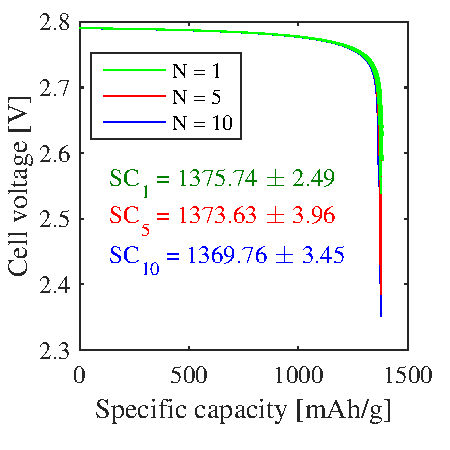
\includegraphics[width=0.5\textwidth]{figures/Petru_N_1_5_10_012016}
	\caption{Variation of the specific area with $N = 10$}
\end{figure}

\chapter{AMES ARC Li-air battery modeling notes}
\section{Learning to implement Petru's equations on Comsol} Relating equations solved by Sahapatsombut (which is implemented in Comsol --by default) to Randflux or Petru's theory. The table lists relationships for cylindrical pores of a single pore size.
Specific area ($a$) is a ratio of accessible surface area to total volume. Assuming cathode made up solid cylindrical fibers,  pores are obtained from empty spaces in these cylindrical fibers. A simple derivation for specific area and porosity ($\epsilon$, it is also referred to as volume fraction) is shown for cathode with a cylindrical morphology.  
\paragraph{Specific Area}
\begin{center}
	\begin{tabular}{|l l l|}
		\hline		
           Parameter &  Petru & Sahapatsombut \\
		$a$  & $\frac{2\sqrt{\epsilon\epsilon_0}}{r_0}$ & $a_0\left(1-\left(\frac{\epsilon_{Li_2O_2}}{\epsilon_{l,0}}\right)^{0.5}\right)$ 	\\					
		\hline
	\end{tabular}
\end{center}
\section{Replication of EIS and discharge curves from Kristian}
Experimental parameters as obtained from \cite{Knudsen2016}
Knudsen reported BET surface area for a Vulcan XC72 to be 235 cm$^2$/mg or 23.5 m$^2$/g which is  much lower than reported in the literature, 245 m$^2$/g \cite{Pantea2003}, 234.9517 m$^2$/g \cite{Lee2006}, 254.0 m$^2$/g \cite{Pantea2001}, 267 m$^2$/g \cite{Yang2004}, 233 m$^2$/g \cite{Gunasekara2015}.
\begin{center}
	\begin{tabular}{|l l l|}
		\hline		
           Parameter &  values & unit  \\
           Volume ($\pi \frac{\phi^2_{diameter}}{2}\times d_{thickness}$) &
           
           
           $2.54475\times 10^{-7} \textrm{ }(0.254475)$ & m$^3$ (cm$^3$)\\
           sample weight & $0.011\textrm{ }(11)$ & g (mg) \\
           BET $SA$   & $23.5\textrm{ }(235)$ &	m$^2$/g (cm$^2$/mg) \\
           $SA$   & $0.2585\textrm{ }(2585)$ &	m$^2$ (cm$^2$) \\           
           $a$  & $1.0158169\times 10^{6}  (\times 10^{4})$ & m$^{-1}$ (cm$^{-1}$) 	\\
           Separator (Whatman QM-A Glass 1pc) & $450$& $\mu$m \\
           Separator (WQM-A 9pc) & $4050$&  $\mu$m\\
           
		\hline
	\end{tabular}
\end{center}
\section{ZnO thickness modeling for Bala}
The thickness of zinc oxide is considered by adding ZnO resistance (through conductivity, $\sigma = \sigma_0e^{\left(\frac{-E}{kT}\right)}$ and through definition of resistance, $R=\int\frac{\rho(r)dr}{A}$) Conductivity of nanostructured ZnO at room temperature is $7.261\times 10^{-7}$ S/cm \cite{Caglar2009}. Assuming pores to be cylindrical in shape with length equal to cathode length.  The cathode skeleton or conducting matrix for the following example is taken to be carbon black (XC-72 --used by Kristian and the impedance response and other measurements are made on these electrodes). 
\subsection{Carbon black electrode approximation} Earlier modeling methods approximated Carbon Black electrode as a cylinder, however, recently many groups have started to model CB with spherical particles. \cite{Vamsci2014,Franco2013a}  (According to Franco, CB should be modeled as Spherical Particles) Carbon electrode allows one to use a cylindrical pore approximation. The cylindrical pore approximation considers that the deposition of the discharge product reduces the pore radius which in turn reduces the available volume for oxygen transport and for discharge product to deposit. The change is porosity is given by 
\begin{equation}
\epsilon\left(t\right)=\epsilon_0\left(\frac{r_{avg}\left(t\right)}{r_{0,avg}}\right)^2
\label{eqn:cylinder_porosity_defn}
\end{equation}
where $r_{avg}\left(t\right)$ is the average radius of $n$ pores at time $t$ and $r_{0,avg}$ is the initial radius of the $n$ pores. $\epsilon\left(t\right)$ is derived in the following way. The initial porosity is given by (assuming cylinder shape of the electrode and that it runs the length of the electrode ),
\begin{equation}
\epsilon_0 =\frac{\pi r^2_{0,avg}L_c}{V}
\label{eqn:cylinder_initial_porosity_defn}
\end{equation}
where $L_c$ is the length of the cathode and $V$ is the total volume of the electrode, it is the assumed volume (assuming a rectangular parallelopiped with side $d$ and length $L_c$, the total available volume $V$ becomes  $V=d^2\times L_c$ ).  The temporal porosity is given by,
\begin{equation}
\epsilon\left(t\right) =\frac{\pi r^2_{avg}\left(t\right)L_c}{V}
\label{eqn:cylinder_temporal_porosity_defn}
\end{equation}
The ratio of eqn. \ref{eqn:cylinder_temporal_porosity_defn} to eqn. \ref{eqn:cylinder_initial_porosity_defn} results in eqn. \ref{eqn:cylinder_porosity_defn}
\paragraph{Voltage drop} The voltage drop across the deposit layer is given by,
\begin{equation}
V_{Li_2O_2} = R_c\times 2\pi r_{avg}\left(t\right) \times \frac{\rho_{Li_2O_2}}{2\pi}\ln{\left[\frac{r_{avg}\left(t\right)}{r_{0,avg}}\right]}
\end{equation}
where $R_c$ is the Faradaic reaction rate. The resistance per unit length $R$ is calculated from the morphology,
\begin{equation}
R = \frac{\rho_{Li_2O_2}}{2\pi}\int_{r_{0,avg}}^{r_{avg}\left(t\right)}\frac{dr}{r}
\end{equation}
after integrating we get,
\begin{equation}
R = \frac{\rho_{Li_2O_2}}{2\pi}\ln{\left[\frac{r_{avg}\left(t\right)}{r_{0,avg}}\right]}
\end{equation}
and the current per unit length is given by,
\begin{equation}
I = 2\pi r_{avg}\left(t\right)  R_c,
\end{equation}
Using the above relations for $R$ and $I$ and using ohm's law ($V=I\times R$); the final equation for $V_{Li_2O_2}$ becomes,
\begin{equation}
V_{Li_2O_2} = R_c r_{avg}\left(t\right)  \rho_{Li_2O_2}\ln{\left[\frac{r_{avg}\left(t\right)}{r_{0,avg}}\right]}
\end{equation}
The voltage drop across the deposit layer according to \cite{Sahapatsombut2013}  is 
\begin{equation}
V_{Li_2O_2}=j_c \overline{R}_{Li_2O_2}\epsilon_{Li_2O_2} 
\end{equation}
where $j_c$ is the current density (A/cm$^2$), $\overline{R}_{Li_2O_2}$ is the interfacial resistance of the film ($\Omega$-cm$^2$), and $\epsilon_{Li_2O_2} $ is the volume fraction of the deposited film. The interfacial resistance can be computed using,
\begin{equation}
\overline{R}_{Li_2O_2} =\rho_{Li_2O_2} \Delta t_{Li_2O_2}
\end{equation}
where $\rho_{Li_2O_2}$ ($\Omega$-cm) is the resistivity and $\Delta t_{Li_2O_2}$ (cm) is the thickness of the film.
Some of the sample calculations are done below to compute the voltage drop 
3\begin{figure}[htb]
	\centering
	\includegraphics[width=0.5\textwidth]{figures/cylinder_pore_model}
	\caption{Cross section of a cylindrical pore model}
\end{figure}
\subsection{Carbon fiber electrode approximation}
A single carbon fiber is assumed to be a cylinder of radius $r_{0,avg}$ and the reaction product is deposited on the solid cylinder. The radii in a carbon fiber electrode increase with deposition, while, the radii in a carbon electrode decreases.
\section{Solvent-in-Salt Electrolyte}
WiSE from Bazant talks about how electrostatic field and the electorstatic energy of the system is different from IL. 
Lithium activity changes inside electrodes. The anode and cathode potentials shift in a SIS, due to change in activity potentials as predicted by Nernst equation.
\section{Battery Prognostics (Future project)}
Lithium platting in Li-ion is possible at high C rates and low temperature. 
\subsection{How to reproduce dendrites predictable}
\subsection{How to model NDE methods in COMSOL}
\subsection{How to model dendrites (non-fractal method)}
\subsection{Couple NDE with Battery simulation}

\section{Requirements for synthetic biochemistry}
\section{Biosciences}
\subsection{Membranes}
\subsection{Synthetic medicine}
\subsubsection{Understating Gene mutation pathway and its expression}


\subsection{Ionization models}
\subsection{}

\newpage
\bibliographystyle{unsrt}
\bibliography{Library_backup_latest}
\end{document}